% Options for packages loaded elsewhere
\PassOptionsToPackage{unicode}{hyperref}
\PassOptionsToPackage{hyphens}{url}
\documentclass[
  american,
  11pt,
]{article}
\usepackage{xcolor}
\usepackage[margin=22mm]{geometry}
\usepackage{amsmath,amssymb}
\setcounter{secnumdepth}{-\maxdimen} % remove section numbering
\usepackage{iftex}
\ifPDFTeX
  \usepackage[T1]{fontenc}
  \usepackage[utf8]{inputenc}
  \usepackage{textcomp} % provide euro and other symbols
\else % if luatex or xetex
  \usepackage{fontspec} % this also loads fontspec
  \defaultfontfeatures{Scale=MatchLowercase}
  \defaultfontfeatures[\rmfamily]{Ligatures=TeX,Scale=1}
\fi
\usepackage{lmodern}
\ifPDFTeX\else
  % xetex/luatex font selection
  \setmainfont[]{Times New Roman}
  \setsansfont[]{Arial}
  \setmonofont[]{Consolas}
\fi
% Use upquote if available, for straight quotes in verbatim environments
\IfFileExists{upquote.sty}{\usepackage{upquote}}{}
\IfFileExists{microtype.sty}{% use microtype if available
  \usepackage[]{microtype}
  \UseMicrotypeSet[protrusion]{basicmath} % disable protrusion for tt fonts
}{}
\makeatletter
\@ifundefined{KOMAClassName}{% if non-KOMA class
  \IfFileExists{parskip.sty}{%
    \usepackage{parskip}
  }{% else
    \setlength{\parindent}{0pt}
    \setlength{\parskip}{6pt plus 2pt minus 1pt}}
}{% if KOMA class
  \KOMAoptions{parskip=half}}
\makeatother
\usepackage{listings}
\newcommand{\passthrough}[1]{#1}
\lstset{defaultdialect=[5.3]Lua}
\lstset{defaultdialect=[x86masm]Assembler}
\usepackage{longtable,booktabs,array}
\newcounter{none} % for unnumbered tables
\usepackage{calc} % for calculating minipage widths
% Correct order of tables after \paragraph or \subparagraph
\usepackage{etoolbox}
\makeatletter
\patchcmd\longtable{\par}{\if@noskipsec\mbox{}\fi\par}{}{}
\makeatother
% Allow footnotes in longtable head/foot
% No table footnotes.

\usepackage{graphicx}
\makeatletter
\newsavebox\pandoc@box
\newcommand*\pandocbounded[1]{% scales image to fit in text height/width
  \sbox\pandoc@box{#1}%
  \Gscale@div\@tempa{\textheight}{\dimexpr\ht\pandoc@box+\dp\pandoc@box\relax}%
  \Gscale@div\@tempb{\linewidth}{\wd\pandoc@box}%
  \ifdim\@tempb\p@<\@tempa\p@\let\@tempa\@tempb\fi% select the smaller of both
  \ifdim\@tempa\p@<\p@\scalebox{\@tempa}{\usebox\pandoc@box}%
  \else\usebox{\pandoc@box}%
  \fi%
}
% Set default figure placement to htbp
\def\fps@figure{htbp}
\makeatother
% definitions for citeproc citations
\NewDocumentCommand\citeproctext{}{}
\NewDocumentCommand\citeproc{mm}{%
  \begingroup\def\citeproctext{#2}\cite{#1}\endgroup}
\makeatletter
 % allow citations to break across lines
 \let\@cite@ofmt\@firstofone
 % avoid brackets around text for \cite:
 \def\@biblabel#1{}
 \def\@cite#1#2{{#1\if@tempswa , #2\fi}}
\makeatother
\newlength{\cslhangindent}
\setlength{\cslhangindent}{1.5em}
\newlength{\csllabelwidth}
\setlength{\csllabelwidth}{3em}
\newenvironment{CSLReferences}[2] % #1 hanging-indent, #2 entry-spacing
 {\begin{list}{}{%
  \setlength{\itemindent}{0pt}
  \setlength{\leftmargin}{0pt}
  \setlength{\parsep}{0pt}
  % turn on hanging indent if param 1 is 1
  \ifodd #1
   \setlength{\leftmargin}{\cslhangindent}
   \setlength{\itemindent}{-1\cslhangindent}
  \fi
  % set entry spacing
  \setlength{\itemsep}{#2\baselineskip}}}
 {\end{list}}
\usepackage{calc}
\newcommand{\CSLBlock}[1]{\hfill\break\parbox[t]{\linewidth}{\strut\ignorespaces#1\strut}}
\newcommand{\CSLLeftMargin}[1]{\parbox[t]{\csllabelwidth}{\strut#1\strut}}
\newcommand{\CSLRightInline}[1]{\parbox[t]{\linewidth - \csllabelwidth}{\strut#1\strut}}
\newcommand{\CSLIndent}[1]{\hspace{\cslhangindent}#1}
\ifLuaTeX
\usepackage[bidi=basic,shorthands=off]{babel}
\else
\usepackage[bidi=default,shorthands=off]{babel}
\fi
\ifPDFTeX
\else
\babelfont{rm}[]{Times New Roman}
\fi
\ifLuaTeX
  \usepackage{selnolig} % disable illegal ligatures
\fi
\setlength{\emergencystretch}{3em} % prevent overfull lines
\providecommand{\tightlist}{%
  \setlength{\itemsep}{0pt}\setlength{\parskip}{0pt}}

\usepackage{pdflscape}
\usepackage{etoolbox}
\usepackage{needspace}
\lstset{basicstyle=\ttfamily\footnotesize,breaklines=true,breakatwhitespace=false,
  columns=fullflexible,keepspaces=true,showstringspaces=false}
\AtBeginEnvironment{longtable}{\footnotesize}
\AtBeginEnvironment{CSLReferences}{\interlinepenalty=10000}
\setlength{\emergencystretch}{8em}
\widowpenalty=10000\clubpenalty=10000
\setlength{\LTpre}{6pt}\setlength{\LTpost}{6pt}
\setlength{\tabcolsep}{5.8pt}
\AtBeginDocument{\hypersetup{colorlinks=true,linkcolor=blue,urlcolor=blue,citecolor=blue}}
\usepackage{hyperref}
\IfFileExists{xurl.sty}{\usepackage{xurl}}{} % add URL line breaks if available
\urlstyle{same}
\hypersetup{
  pdftitle={GI-TBC: a Gini-interval tailored branch-and-cut algorithm for equitable bicycle redistribution},
  pdflang={en-US},
  hidelinks,
  pdfcreator={LaTeX via pandoc}}

\title{GI-TBC: a Gini-interval tailored branch-and-cut algorithm for
equitable bicycle redistribution}
\author{}
\date{14 November 2026}

\begin{document}
\maketitle

{
\setcounter{tocdepth}{2}
\tableofcontents
}
\clearpage

\subsection{Abstract}\label{abstract}

Static bicycle redistribution must realize an equitable final inventory
through routes with empty departures, prefix capacity and paid handling,
including loaded returns. We develop GI-TBC, an exact method connecting
shared inventory states, objective products, movement and nonzero visits
with complete true-Gini interval coverage. A compact alternative
preserves the joint local hull with at most five legal stock supports
and a separate binary-product layer, under an explicit full-model
interface condition. The historical breadth panel gives GI-TBC 9/12
certificates versus 7/12 for each compact control; a positive-resource
panel gives 4/8 versus 0/8. In a new same-build six-input representation
comparison, B certifies 3/6 and compact C166 2/6. C166 improves two open
primal endpoints but weakens all three large-instance proof endpoints,
so B remains the main method. Reconstructed physical fleets and global
lower bounds also give continuous-weight quality guarantees: one fixed
fleet is within an absolute objective tolerance of 1.00002e-7 throughout
its covered range, while other families exhibit supported plan switches
or wide unresolved bands. Two-sided route-time bounds establish strict
optimal-objective improvement even for open instances. These finite,
numerically qualified results distinguish information-preserving
representations, complete computational value and useful bounded
decisions; the controls do not establish an independent speed advantage
from external interval scheduling.

\subsection{1. Introduction}\label{introduction}

Redistribution vehicles can improve station availability only when the
chosen inventory vector can be realized by feasible routes and loading
operations. Supply must be collected before it is delivered, capacity
applies at every route prefix, and handling consumes the same time
budget as travel. When equity is measured by inventory-to-target ratios,
the final inventory vector also determines both the numerator and
denominator of the Gini coefficient. These dependencies make routing and
inventory allocation inseparable.

We study static bicycle redistribution with empty vehicle departure,
loaded return, and at most one nonzero one-way service at each station.
The objective combines inventory-to-target ratio-Gini dispersion and
weighted relative target deviation. The operational model and HGA-TGBC
heuristic framework originate in the available same-problem author
manuscript (\emph{Equity-Aware Bike Repositioning in Station-Based
Bike-Sharing Systems} 2026). Our exact method reuses its decoder within
a finite startup procedure and supplies the bounds and complete coverage
needed for certification.

The research question is how a common inventory representation can
connect allocation and routing, support a complete exact method, and
yield decisions whose quality can be bounded. Three connected
contributions address it. First, a shared stock state represents the
objective product, absolute movement and nonzero visits. Under the
inherited unique one-way service rules, integer stock implies integer
service quantities. We further characterize the joint local graph: at
most five legal stock supports preserve its continuous convex hull,
while a separate absolute-stock binary-product layer preserves integer
exactness. The resulting common LP projection survives embedding only
when all other state uses pass through the declared interface. This
identifies both a compact representation and its precise boundary.

Second, GI-TBC combines inventory/service connections and physical valid
inequalities with an own feasible startup and complete true-Gini
interval control. Objective-preserving physical extensions, cutoff
complements and complete region coverage establish correctness. The
implementation supplies the full method, including exact continuation at
depth/width guards. Custom valid rows are static; Gurobi performs
branch-and-cut inside each canonical model. P, own-start PS,
strengthened root-only control, complete B and the separate proof
extension answer different formulation, startup and architecture
questions. The compact representation is evaluated as the separately
named C166 candidate; it does not change B's definition.

Third, computational evidence and certified decision analysis use both
feasible fleets and qualified problem bounds. The complete package
improves finite certificate counts over the specified compact controls,
with adverse endpoints and open cases retained. An offline archive of
fully reconstructed physical fleets yields feasible upper envelopes and
concavity-based lower bands over continuous objective-weight intervals.
Controlled route-horizon pairs yield two-sided bounds on the improvement
in the optimal objective, including pairs where neither optimum is
certified. These decisions concern inventory-to-target ratio dispersion
and target deviation. They do not imply demographic fairness, monetary
benefit, a complete Pareto frontier or an independent speed gain from
the outer controller.

\subsubsection{1.1 Relation to previous
work}\label{relation-to-previous-work}

Static bike redistribution has been studied under several target,
service and vehicle conventions. Raviv et al.~develop static
repositioning models; Chemla et al.~study static rebalancing; Erdogan et
al.~address demand intervals and an exact rebalancing algorithm (Raviv
et al. 2013; Chemla et al. 2013; Erdoğan et al. 2014, 2015). Schuijbroek
et al.~connect inventory requirements to routing (Schuijbroek et al.
2017). Forbidden temporary operations, repeated visits, robust inventory
requirements and demand-interval disjunctions give related but different
feasible sets (Bruck et al. 2019; Bulhões et al. 2018; Bruck et al.
2025; Ikonen et al. 2025). The HGA-TGBC manuscript is the direct
same-problem antecedent; the other studies supply routing and
formulation context rather than matched performance baselines.

Station-ratio dispersion measures a different object from
vehicle-workload equity (Matl et al. 2018). Qiao et al.~balance task
durations in a coordinated two-echelon rebalancing framework (Qiao et
al. 2026). Caggiani et al.~consider free-floating electric
micromobility, battery swapping and a modified Gini measure involving
availability and state of charge, with zonal fair targets (Caggiani et
al. 2026). Their accessible abstracts identify these equity objects and
operation settings; the unread complete formulations do not support
equivalence or dominance claims. Here zero Gini means equal proportional
station inventory, which can still represent inadequate stock. The
deviation term separately rewards approaching targets.

McCormick envelopes and convex epigraphs are standard tools (McCormick
1976; Boyd and Vandenberghe 2004). Gupte et al.~study unary/binary
reformulations and relaxations of integer-continuous single-product sets
(Gupte et al. 2013). Köppe et al.~develop finite block values, linking
polyhedra and an aggregate representation (Köppe et al. 2008). Our
connection is the use of one final-stock state across the objective,
absolute movement and nonzero-service indicator, within this physical
routing problem. Embedding and piecewise-linear formulations provide
established endpoint, encoding and convexification tools (Vielma 2018;
Huchette and Vielma 2023). Our compact result applies these tools to the
jointly visible movement, visit and product functions, including their
discrete service jump, and establishes the interface needed to embed the
replacement. Neither binary expansion, finite disjunction, endpoint
convexification nor spatial partitioning is claimed as new. The
state-penalty comparison in Supplement S6 applies Jensen's inequality
and a direct projection construction; the complete route model is not
the hull of an isolated product block.

\subsection{2. Physical model and
objective}\label{physical-model-and-objective}

Let \(N\) contain \(n\) stations and let \(0\) be the depot. Station
\(i\) has integer initial inventory \(b_i\), capacity \(C_i\), positive
target \(D_i>0\), and weight \(\omega_i\ge0\). Vehicle \(k\) has
capacity \(Q_k\) and route-duration limit \(T\). Routes depart empty. A
station can be served by at most one vehicle, in one direction, with a
nonzero operation. Loaded return is allowed and its unloading time is
counted. The depot enters neither target deviation nor dispersion.

The computational text format stores integer targets. All present test
targets also satisfy \(D_i\le C_i\), a data convention rather than an
additional physical constraint; the inventory capacity bounds apply to
\(b_i,Y_i\).

With pickup \(p_{ki}\) and delivery \(d_{ki}\),

\[
Y_i=b_i+\sum_k(d_{ki}-p_{ki}),\qquad
R_k=\sum_i(p_{ki}-d_{ki})\in[0,Q_k],\qquad
\sum_iY_i=\sum_i b_i-\sum_kR_k.
\]

Thus total final station inventory is bounded above by \(B=\sum_i b_i\),
rather than fixed at \(B\). Vehicle capacity limits the instantaneous
prefix load, rather than cumulative pickup. If pickup and
unloading/delivery take \(t_p,t_d\) per unit, complete handling time is

\[
t_p\sum_i p_{ki}+t_d\left(\sum_i d_{ki}+R_k\right)
=(t_p+t_d)\sum_i p_{ki}.
\]

Travel plus this quantity cannot exceed \(T\). The tested distance
convention is Euclidean travel time from serialized metre coordinates at
1.5 m/s. Inventory, route, assignment, direction and prefix-load logic
retain their original integer domains. Continuous pickup/delivery
variables preserve the integer physical operations because unique
one-way service and integer \(Y_i\) fix the sole inventory difference.
Appendix A gives the complete formulation and embedding proof.

Define

\[
r_i=Y_i/D_i,\quad S=\sum_i r_i,\quad
A=\sum_{i<j}|r_i-r_j|,\quad
P=\sum_i\omega_i|r_i-1|,
\] \[
G=\begin{cases}A/(nS),&S>0,\\0,&S=0,\end{cases}
\qquad F=G+\lambda P,\quad\lambda\ge0.
\]

This is ratio dispersion and two-sided relative target deviation. It is
not a direct measure of population equity, rental failure or travel
burden. Put \(\Omega=\sum_i\omega_i>0\), \(P_{\rm avg}=P/\Omega\) and
\(\rho=\lambda\Omega\). Then \(F=G+\rho P_{\rm avg}\). The generator
normalizes weights by their maximum, so equal \(\lambda\) across inputs
does not hold \(\rho\) fixed. The breadth panel retains this convention;
the resource panel fixes \(\rho=1\), and the weight study varies
\(\rho\) within fixed physical configurations.

For positive total shortage \(s=\sum_iD_i-\sum_ib_i>0\), positive
weights and \(\lambda>0\) (equivalently \(\rho>0\)), let
\(a=\min_i\omega_i/D_i>0\). Nonnegative loaded return yields

\[
P\ge a\sum_i|D_i-Y_i|\ge a\left|\sum_iD_i-\sum_iY_i\right|\ge as,
\qquad F\ge\lambda as=\rho as/\Omega>0.
\]

We use this established stock-shortage construction to guarantee
positive objectives in the resource study, without filtering on observed
difficulty. It does not guarantee a binding route horizon. With all
other physical and objective data fixed, \(T_1\le T_2\) gives
\(X(T_1)\subseteq X(T_2)\) and \(F^*(T_2)\le F^*(T_1)\). Finite-budget
primal/dual endpoints and runtimes need not be monotone.

\subsection{3. Shared inventory states and
GI-TBC}\label{shared-inventory-states-and-gi-tbc}

\subsubsection{3.1 Discrete states and implicit service
integrality}\label{discrete-states-and-implicit-service-integrality}

For the legal finite inventory domain \(\mathcal Y_i\), binary selectors
\(s_{iy}\) and continuous \(q_{iy}\) represent stock and products on a
Gini interval \([\alpha,\beta]\):

\[
\sum_y s_{iy}=1,\quad Y_i=\sum_y ys_{iy},\quad
\alpha s_{iy}\le q_{iy}\le\beta s_{iy},\quad
\sum_yq_{iy}=g,\quad Z_i=\sum_y yq_{iy}.
\]

At an integer state, \(Z_i=gY_i\). The objective epigraph uses

\[
H_{ij}\ge r_i-r_j,\quad H_{ij}\ge r_j-r_i,\qquad
e_i\ge r_i-1,\quad e_i\ge1-r_i,
\] \[
\sum_{i<j}H_{ij}\le n\sum_i Z_i/D_i,\qquad
\min f=g+\lambda\sum_i\omega_i e_i.
\]

For \(S>0\), integer state selection makes the numerator inequality
imply \(g\ge G_{\rm true}\), so every integer completion satisfies
\(f\ge F_{\rm true}\). Conversely a physical fleet assigned to its
true-G interval has an objective-preserving extension: select its final
inventories, set \(g=G_{\rm true}\), set each selected \(q_{iy}=g\), and
use the true absolute differences and deviations. At \(S=0\), all ratios
are zero and \(g=0\) supplies the physical extension. Valid domain and
strengthening rows retain that extension, as established in Appendix A.

Let \(z_{ki}\) be the binary service assignment. The same state supports
the service equations

\[
\sum_kp_{ki}=\sum_y(b_i-y)^+s_{iy},\quad
\sum_kd_{ki}=\sum_y(y-b_i)^+s_{iy},\quad
\sum_kz_{ki}=\sum_{y\ne b_i}s_{iy}.
\]

These links connect objective mixtures to movement and service. They are
not the convex hull of all vehicle routes. In isolation, a finite-state
product block with the same extreme stock bounds projects to the
McCormick rectangle: its four corner graph points give one inclusion,
and every state line lies in the rectangle hull, giving the other. An
advantage must therefore come from the links, domain information or
complete search, rather than the VD-P label alone.

\Needspace{8\baselineskip}

\textbf{Lemma 1 (implicit service integrality).} Suppose initial and
final inventories are integer, a station is assigned to at most one
vehicle, and a binary direction permits either pickup or delivery at its
unique service. Continuous pickup and delivery variables then take
integer values at every integer solution of the remaining model.

\textbf{Proof.} An unassigned vehicle has zero quantities. At the unique
assigned vehicle, pickup direction fixes delivery to zero, so inventory
balance gives \(p_{ki}=b_i-Y_i\). Delivery direction fixes pickup to
zero and gives \(d_{ki}=Y_i-b_i\). Each is integer. Integer load
variables are unnecessary for this implication. The claim concerns
integer feasible solutions; it does not equate the continuous
relaxations of alternative formulations. \(\square\)

For an integer service, total movement is \(|b_i-Y_i|\), and nonzero
one-way service occurs exactly when \(Y_i\ne b_i\). Hence the shared
equations above reproduce the original operations without changing the
physical problem. They also couple fractional inventory mixtures to the
movement and visits that must support them.

\paragraph{3.1.1 A compact shared-state
representation}\label{a-compact-shared-state-representation}

On a legal contiguous stock domain \(\mathcal Y_i=\{l_i,\ldots,u_i\}\),
define \(m_i(y)=|b_i-y|\), \(v_i(y)=\mathbf1\{y\ne b_i\}\), and the
common local object

\[
\mathcal H_i=\operatorname{conv}\{(y,m_i(y),v_i(y),g,gy):y\in\mathcal Y_i,\ g\in[\alpha,\beta]\}.
\]

The relevant physical coordinates are inventory, aggregate movement,
aggregate visits, \(g\) and \(Z_i\). Balance linearly recovers aggregate
pickup and delivery from inventory and movement. The relaxed VD-P block
and A/B links represent this joint object; independently convexifying
service and the product can instead use inconsistent inventory mixtures.

\textbf{Compact joint-state proposition.} For
\(0\le\alpha\le\beta\le1\), let

\[
\mathcal K_i=\{l_i,u_i\}\cup\bigl(\{b_i-1,b_i,b_i+1\}\cap\mathcal Y_i\bigr).
\]

Replacing \(\mathcal Y_i\) by these at most five legal supports
preserves \(\mathcal H_i\). Continuous perspective weights on those
supports, combined with an independent absolute-\(Y_i\) binary-product
layer, preserve B's integer physical projection, original objective and
common raw LP projection, provided every other deleted-state use passes
through the common interface.

\textbf{Proof sketch.} On the legal donor, initial singleton and
receiver pieces, all three functions \(y,m_i(y),v_i(y)\) are affine. An
interior integer stock is interpolated between its piece's legal
endpoints at the same \(g\), preserving \(gy\) as well. The converse
uses the legality of every retained support. The bit layer makes
\(Z_i=gY_i\) exact at integer stocks. Its relaxed projection contains
every true stock/product graph point, hence their convex hull; its
disjoint auxiliary variables therefore do not change the breakpoint
block's common LP projection. Intersecting with unchanged outside
constraints preserves this equality under the stated interface
condition. Appendix A.9 supplies the construction, both directions,
sizes and failure cases. \(\square\)

Continuous breakpoint weights and integer \(Y_i\) alone do not enforce
the product, and binary breakpoint weights would delete legal interior
stocks. B keeps its original \(e_i\) epigraph, so target deviation is
not an additional shared-state function here. Exact state penalties,
threshold counts, vehicle-state assignment or holed stock domains need
additional supports or restrictions. The candidate C166 applies only
this representation change, with the full B lifecycle and own startup.
Equal raw LP projections do not imply identical presolve cuts, branch
decisions or complete costs.

\subsubsection{3.2 Ordered supply and support/handling
information}\label{ordered-supply-and-supporthandling-information}

Let \(\tau\) be metric travel time and \(h=t_p+t_d\). For each receiving
station \(j\), define

\[
\mathcal C_{kj}=\{i\ne j:\tau_{0i}+\tau_{ij}+\tau_{j0}+h\le T\}.
\]

\Needspace{8\baselineskip}

\textbf{Proposition 1 (ordered supply compatibility).} Every physical
fleet with empty departure satisfies

\[
d_{kj}\le\sum_{i\in\mathcal C_{kj}}p_{ki}.
\]

\textbf{Proof.} Label the units collected by a vehicle. In route order,
match each delivered unit to an earlier collected unit that has not yet
been delivered. Nonnegative prefix loads guarantee such a match. A unit
delivered at \(j\) from source \(i\) entails the ordered subsequence
\((0,i,j, 0)\), whose travel lower bound follows by metric shortcutting.
Collecting at least that unit incurs handling of at least \(h\),
including delivery or final unloading. Thus its source lies in
\(\mathcal C_{kj}\). Counting distinct matched units proves the
inequality. Unmatched collected units can return to the depot.
\(\square\)

For a set \(W\) of served stations, let \(\tau(W)\) be the shortest
depot tour through \(W\), computed by explicit orders for pairs or
triples. Write \(P_k^{\rm pick}=\sum_i p_{ki}\). Nonzero integer service
and empty departure give

\[
|W|\le\sum_{i\in W}(p_{ki}+d_{ki})\le2P_k^{\rm pick},\qquad
P_k^{\rm pick}\ge\lceil |W|/2\rceil.
\]

Consequently \(\tau(W)+h\lceil|W|/2\rceil>T\) rules out serving all of
\(W\) with that vehicle. Otherwise a conditional duration inequality
combines the tour lower bound and pickup handling. Supply for \(W\) may
come from outside \(W\); cumulative pickup is not bounded by \(Q_k\).
Appendix A gives the exact conditional coefficients, deactivation proof
and finite selection rule. GI-TBC keeps pair support uniformly and omits
triple support. These rows strengthen necessary physical conditions
without replacing route-prefix capacity.

\subsubsection{3.3 Complete startup and interval
search}\label{complete-startup-and-interval-search}

The startup \(H\) is a finite construction and descent procedure. It
completes a joint insertion and 24 shuffled station/separator orders
plus a constructive order, fully decodes them, applies guided
first-improvement descent, and closes physical quantity/insertion and
neutral balanced/exchange moves. The active path has no genetic
generations. It provides a verified feasible upper bound and a possible
MIP Start; it is never credited with a positive lower bound. Each GI-TBC
and paid-start compact run pays for its own complete \(H\).

The controller starts from the complete potentially improving domain
\([0,\min\{U,(n-1)/n\}]\). It maintains incumbent epoch, valid cutoff
complements and complete interval coverage. A local bound is used only
for its model, interval, cutoff and qualified source. Split children
replace a parent atomically only after complete coverage and both
results are checked. NEXT and child-target values are requests, rather
than proof that a milestone was reached.

\par\medskip\noindent\begin{minipage}{\linewidth}

\begin{lstlisting}
Algorithm 1  GI-TBC (B)
Input: physical instance, lambda/weights, common deadline; fixed .08 AM rule,
       depth 8, minimum width 1e-4, numerical policy epsilon=1e-7.
Output: verified own fleet, physical U, qualified L, CERT or OPEN and cover.
1 Complete own H and verify the fleet; initialize U and incumbent epoch e=0.
2 Cover [0,min(U,(n-1)/n)] (also [0,0]); retain independent global floor 0.
3 While a relevant open region exists and the common deadline permits:
    select on the minimum-bound plateau, cycling widest-first (B.2);
    rebuild its canonical model at current epoch/cutoff c=U when necessary;
    qualify its complete LP and merge its applicable same-region floor.
    If proved infeasible or fathomable: retain the scoped closure; else:
      apply NEXT: requeue if noncontrolling, or request a parent-MIP target
      equal to the next strictly larger open-region bound (B.3);
      if NEXT permits lookahead and depth/width permit, solve both child LPs;
      split atomically if either is infeasible or the finite AM rule passes;
      otherwise request parent MIP to the valid child minimum when strict;
      if guarded or without strict child improvement, run full parent MIP.
    After each Native return, finalize/qualify its actual bound and source;
    verify fleet improvements, update U/epoch and invalidate stale artifacts;
    install both covering children, retain a scoped closure, or requeue the
    parent according to the returned evidence (ProcessLeaf, Appendix B.0).
    Recompute the full-cover minimum including cutoff-complement floors.
    On TimeLimit retain unresolved coverage; on failed qualification stop.
4 FinalizeAndUpdateCover retains every unresolved obligation (Appendix B.0).
  If native proof is rejected, final qualification restores the unresolved
  physical domain and independent floor 0; no dependent proof is credited.
5 Release Native resources; finalize the selected fleet's physical check.
  Apply the independent exact-zero rule or qualified full-cover gap rule;
  complete required output and return CERT, otherwise OPEN with its bounds.
\end{lstlisting}

\end{minipage}\par\medskip

\Needspace{8\baselineskip}

\textbf{Proposition 2 (coverage).} In ideal arithmetic, a controller
that preserves complete improving-domain coverage, retains valid
bound/cutoff complements and closes a region only by an applicable proof
provides a valid global lower bound. If it closes all relevant regions
against a verified \(U\), it proves optimality to its declared
certificate margin.

\textbf{Proof.} Every improving physical solution belongs to the root
domain because \(F\ge G\) and \(G\le(n-1)/n\). A valid interval
restriction and cutoff cover its regional solutions; the cutoff
complement has floor equal to that cutoff. A complete split preserves
the union. Taking the minimum over the valid regional floors and
complements therefore bounds every physical solution from below. Closure
against \(U\) eliminates every possible improvement to the margin.
Revoking a source requires removing every conclusion that depends on it;
an independent full-domain bound remains valid. \(\square\)

The proof's source-dependency requirement is not a claim of a general
online revocation engine. The frozen scheduler accumulates same-unit
bounds monotonically. Its actual final qualification rejects affected
native proof dependencies and conservatively restores the unresolved
physical domain; Appendix B.4 distinguishes that fallback from ideal
proof accounting. This proposition does not turn floating-point native
calculations into exact rational proofs. Numerical qualification,
physical objective agreement and lifecycle evidence are additional
implementation conditions. The final implementation separates ordinary
positive-objective native/outer certificates from the independent zero
rule. Supporting material records numerical anomalies and version
corrections without making them algorithmic contributions.

The depth and width guards limit extra partitioning, then retain a full
parent MIP continuation. In ideal arithmetic, complete terminal
solutions on the bounded integer domains and valid coverage yield the
corresponding finite proof. Under the actual common deadline an
unresolved terminal obligation returns OPEN; the guards themselves
establish no certificate.

\subsubsection{3.4 Numerical qualification and
termination}\label{numerical-qualification-and-termination}

\textbf{Independent zero termination.} Under the stated nonnegative
objective premises, a complete physically verified fleet with exact
objective zero is globally optimal, independently of the native search
source.

\textbf{Proof.} For every original physical solution, \(F\ge0\). The
verified fleet gives \(F^*\le0\), so \(0\le F^*\le0\). With positive
\(\lambda\) and positive weights, integer equality \(Y_i=D_i\) for every
station is a sufficient exact-zero condition. More generally equal exact
ratios give zero Gini, and every positive-weight penalized station must
meet its target. The implementation checks these conditions using
integer stock arithmetic, then repeats the complete physical-fleet
verification. A merely small positive floating objective does not
establish exact zero. \(\square\)

The numerical \(\varepsilon\)-certificate policy is separate. A
source-rejected positive solution without a sufficient independent bound
remains open. Certification cost includes the verification needed to
establish the proof, normal native cleanup and required output. A later
offline audit cannot backdate a production proof.

\subsubsection{3.5 A separately paid proof-only inventory
source}\label{a-separately-paid-proof-only-inventory-source}

The frozen enhancement E+ augments GI-TBC/B with an independently
computed, qualified inventory lower bound. It uses the run's own first
canonical root, actual supported inventories and valid final-stock total
bounds. On an epigraph interval \([\gamma_L,\gamma_U]\), its objective
and domain are

\[
 \min_Y\;\max\{\gamma_L,G_{\rm true}(Y)\}
       +\lambda\sum_i\omega_i|Y_i/D_i-1|,
 \qquad G_{\rm true}(Y)\le\gamma_U.
\]

The lower interval endpoint constrains the epigraph; it does not impose
\(G_{\rm true}\ge\gamma_L\). At \(S=0\), \(G_{\rm true}=0\). The
inherited exact hard-total dynamic program and one uniform RN16384
producer retain their original absolute price gap, zero/fallback
handling, scope qualification and global deadline. This is an
application of established integer-inventory, normalization and
proof-ledger techniques, not a new general fractional-programming or
convex-hull theorem.

Only an applicable proof ledger consumes the returned floor. Formal
Native rows, raw AM bounds, hints, Starts and branching inputs keep
their intended B design. On a common domain, independent bounds combine
by maximum; complete covering regions combine by minimum, including each
source's cutoff complement. Helper rejection supplies no new floor and
retains the independent B information. Every E+ run pays its own H,
root, DP/RN work and qualification. That cost changes remaining search
time, and legitimate early certification can change the finite
trajectory. Preserving the formal expression therefore does not
guarantee identical B/E+ physical incumbents or solve times.

The C++ complete-method implementation and the historical Python
inventory helper are separately identified in the supplement. No
per-instance, source, scale, machine-speed or elapsed-time enhancement
switch is used. Stable B and the paper recommendation remain separate
from released defaults.

E+ evidence is confined to its separately registered runs. B/P
solver-Seed repeats do not retest the helper or establish its
robustness. The inventory source's mathematical validity, numerical
qualification and net value for the complete paid method remain separate
questions.

\subsection{4. Computational design}\label{computational-design}

The main comparisons use the same physical problem and original
objective. P is the independent cold compact model; PS pays its complete
own H and maps only its own fleet into the original compact model;
GI-TBC pays its complete own H, model construction, verification,
interval search and proof/output. No solution, bound, tree or Start
crosses methods, Seeds, objective weights or physical configurations.
Gurobi 13.0.2 uses one thread and fixed processor affinity on an Intel
i7-12700KF Windows host. H seed 20260626 is held fixed; each study
registers its Gurobi Seeds separately. Same Seed does not mean different
models follow the same random trajectory.

Each comparison answers a different question. P/PS measures the complete
cost and benefit of an own feasible startup in the compact model. The
strengthened root-only control retains shared-state and physical rows
and its own startup, using native branch-and-cut on the unsplit root
domain; its comparison with complete B tests the additional external
control package. B/P and B/PS evaluate the integrated exact method. E+/B
prices a separate inventory-proof source and its lower-bound
contribution. C166/B keeps the complete flow and changes the
shared-state representation, testing whether equal raw LP information
can be carried at a better complete cost. The historical controls and
the new representation comparison retain separate versions, inputs and
denominators.

The fixed-source protocol was committed before once-only generation. Six
known roles and six new draws form a twelve-input breadth panel (four
each at \(n\in\{15,20,35\}\)); CITI, CABI and Divvy supply archived
station geometry/capacity. Ten new draws in total include four
additional shortage bases at \(n\in\{20,35\}\), each paired at two
transparently designed route horizons. Targets, initial stock, weights
and depot are synthetic or transformed; this is not observed demand, a
new source, or independent population sampling. Every selected source
row and serialized input is disclosed.

Breadth retains \(\lambda=.15\). Resource pairs fix \(\rho=1\) and alter
only T; the two extra weight levels \(\rho\in\{.5,2\}\) reuse the
matching \(\rho=1\) baseline at two preselected physical configurations.
AM and mechanism defaults share only exactly matching
input/T/weight/Seed/cap/configuration runs. The earlier main panels use
Seed 0; four preselected full-method triplets and small overlapping
AM/mechanism blocks use Seed 1. They are finite repeated observations,
not independent new inputs or an estimated runtime distribution. The
later six-input archived-source cohort uses Seed0 for its B/E+/P
comparison and Seeds1/2 for the complete B/P confirmation in §5.5. The
additional 24 commands and offline feasible targets are frozen together;
this extends existing Seed research on exposed inputs rather than
supplying new unseen inputs.

For each new resource base, let \(d_{\max}\) be its maximum serialized
station-to-depot distance and \(M\) its vehicle count. Before
optimization, the route horizons were fixed by

\[
\begin{aligned}
T_{\rm base}&=2d_{\max}/1.5+120\sum_{i\in N}\max(b_i-D_i, 0)/M,\\
T_1&=300\left\lceil\frac{\max(1800,.75T_{\rm base})}{300}\right\rceil,\\
T_2&=300\left\lceil\frac{1.5T_1}{300}\right\rceil.
\end{aligned}
\]

This input-based rule uses geometry, initial stock, targets and fleet
size; it supplies neither a binding-horizon guarantee nor an
outcome-dependent difficulty filter. The weight study preselects
R-B20-S-T1 and R-X35-S-T2. Within each T pair, every datum except T is
identical.

Caps are 600/1200/2400 s by size; every open certificate time remains
null. Actual production, postverification and total clocks are retained
separately. Native proof qualification and physical original-objective
endpoints follow the registered numerical policy in §3.4 and Appendix
A.7. Rejected native sources cannot support a bound. A current run can
still qualify its own independently finalized exact-zero certificate
under that policy; this basis and any rejected source are reported
separately. Both-certified time differences are substantive when at
least max(10s, 10\% of the faster time); numerical values and the
conditioned intersection denominator accompany the classification.

\Needspace{20\baselineskip}

\textbf{Table 1. Registered studies, observations and shared defaults.}

{\def\LTcaptype{none} % do not increment counter
\begin{longtable}[]{@{}
  >{\raggedright\arraybackslash}p{(\linewidth - 4\tabcolsep) * \real{0.3333}}
  >{\raggedright\arraybackslash}p{(\linewidth - 4\tabcolsep) * \real{0.3333}}
  >{\raggedright\arraybackslash}p{(\linewidth - 4\tabcolsep) * \real{0.3333}}@{}}
\toprule\noalign{}
\begin{minipage}[b]{\linewidth}\raggedright
Study
\end{minipage} & \begin{minipage}[b]{\linewidth}\raggedright
Configurations / observations
\end{minipage} & \begin{minipage}[b]{\linewidth}\raggedright
Purpose
\end{minipage} \\
\midrule\noalign{}
\endhead
\bottomrule\noalign{}
\endlastfoot
Breadth & 12 physical inputs / 36 methods & Sources, stock regimes and
scales \\
Positive-resource pairs & 4 bases, 8 physical configurations / 24
methods & \(\rho=1\), guaranteed positive objective \\
Weights & 2 physical configurations, 2 extra rho levels / 12 methods &
Relative method dependence on objective weight \\
AM & 4 roles, 2 extra thresholds / 8 methods & Observed gates/actions
and complete cost \\
Mechanisms & 4 roles, 4 contrasts / 16 methods & Conditional
formulation/control effects \\
Earlier second Seed & 12 main+4 AM+8 mechanism methods & Preselected
limited repeat check \\
Archived-source Seed 0 cohort & 6 inputs / 18 B, E+, P method
observations & Complete main method and separate proof extension \\
Exposed-cohort Seeds1/2 & 24 new B/P arms, plus 12 historical Seed0 B/P
arms & Six inputs; three within-input paired observations \\
Compact shared-state comparison & 6 exposed inputs / 12 fresh same-build
B/C166 Seed0 arms & Equivalent common LP information and complete-method
costs \\
\end{longtable}
}

\subsection{5. Complete-method, resource and weight
results}\label{complete-method-resource-and-weight-results}

\subsubsection{5.1 Current main panel and historical
context}\label{current-main-panel-and-historical-context}

\Needspace{8\baselineskip}

\textbf{Table 2. Qualified certificates in the main Seed 0 panels.}

{\def\LTcaptype{none} % do not increment counter
\begin{longtable}[]{@{}llll@{}}
\toprule\noalign{}
Panel & GI-TBC & P & PS \\
\midrule\noalign{}
\endhead
\bottomrule\noalign{}
\endlastfoot
Breadth & 9/12 & 7/12 & 7/12 \\
Resource pairs & 4/8 & 0/8 & 0/8 \\
\end{longtable}
}

Certificates in this table require formal performance eligibility.
Earlier evidence retains its own source and policy: the two-Seed breadth
study obtains 17/24 versus P 9/24 and PS 4/12; the earlier final
confirmation obtains 12/14 versus P 9/14 and PS 2/4. These are separate
panels and repeated observations, and are not pooled with the current
denominators. The earlier breadth study also retains its disclosed
source-reduced own-zero observation outside formal timing counts.

\Needspace{8\baselineskip}

\textbf{Table 3. Certificate-time comparisons conditioned on both
methods certifying.}

{\def\LTcaptype{none} % do not increment counter
\begin{longtable}[]{@{}lllll@{}}
\toprule\noalign{}
Panel & Other & Both certified & GI-TBC W / L & Geo Other / GI-TBC \\
\midrule\noalign{}
\endhead
\bottomrule\noalign{}
\endlastfoot
Breadth & P & 7 & 6 / 0 & 11.3534 \\
Breadth & PS & 7 & 4 / 1 & 4.22522 \\
Resource pairs & P & 0 & 0 / 0 & n/a \\
Resource pairs & PS & 0 & 0 / 0 & n/a \\
\end{longtable}
}

Time ratios and substantive time wins/losses in this table condition on
both methods qualifying a certificate; their intersection sizes are
shown explicitly. A ratio above 1 means a lower GI-TBC certificate time
on this conditioned subset. An open cap supplies no certificate time and
enters neither the ratio nor these time-win counts. Certificate-only
differences and open endpoints remain in the complete panel.

The new positive-objective certificate cases include N-B15-B, N-X15-S
and N-C20-U. On N-B15-B, GI-TBC takes 24.0684 s versus P 279.663 s and
PS 306.307 s. On N-X15-S the corresponding times are
10.2683/538.867/401.931 s. GI-TBC certifies N-C20-U in 265.529s while P
and PS remain open. These observations retain the independent cost of
each complete method.

Paid startup and the subsequent method have distinct effects. On X-35-B,
PS certifies in 7.45014 s versus GI-TBC 17.9046 s, a substantive PS
reversal under the declared rule. On N-X20-B, PS 6.08515 s and GI-TBC
7.45537s differ by less than 10 s, so the nominal ordering is not
substantive. All twelve breadth PS/GI-TBC pairs independently complete H
with matching semantic and fleet hashes; the complete post-startup
packages can still behave differently.

GI-TBC remains open on K-20-S, K-35-U and N-B35-S. K-35-U exposes an
opposed-endpoint result: P has the lower U, 0.664747 versus GI-TBC
0.692854, while GI-TBC has the higher L, 0.565766 versus P 0.335556. No
single endpoint-dominance or certificate-time claim follows. On N-B35-S,
GI-TBC improves both endpoints over P and PS but still leaves a positive
proof gap. These qualified limits accompany the certification gains.

N-X20-B cold P has a rejected native bound source and an own zero
feasible objective. Its 24.0892 s qualified certificate uses the
separately finalized nonnegative full-domain floor, not the rejected
native proof. The complete cost and rejection records remain. This
current-policy independent-zero certificate does not retroactively
change the separately preserved historical exclusion above.

The complete paired interpretation, including substantive reversals and
conditioned runtime statistics, is given in the stage decision and the
full supplement. Smaller signed gap alone does not establish endpoint
dominance: U and L are compared separately. No cap is substituted for a
certificate time.

\subsubsection{5.2 Positive objectives and physical resource
pairs}\label{positive-objectives-and-physical-resource-pairs}

All four serialized shortage bases have positive weights, a strictly
positive analytic floor, and both local donor and receiver stations
before movement. Relaxing T enlarges the feasible set; the observed
feasible plans, qualified bounds and proof progress test how the methods
use that resource, not a causal effect of n alone. The physical
operation records distinguish travel, handling, returned stock, prefix
peaks and route-duration utilization.

\Needspace{8\baselineskip}

\textbf{Table 4. Input-based positive-objective resource design.}

{\def\LTcaptype{none} % do not increment counter
\begin{longtable}[]{@{}
  >{\raggedright\arraybackslash}p{(\linewidth - 10\tabcolsep) * \real{0.1667}}
  >{\raggedright\arraybackslash}p{(\linewidth - 10\tabcolsep) * \real{0.1667}}
  >{\raggedright\arraybackslash}p{(\linewidth - 10\tabcolsep) * \real{0.1667}}
  >{\raggedright\arraybackslash}p{(\linewidth - 10\tabcolsep) * \real{0.1667}}
  >{\raggedright\arraybackslash}p{(\linewidth - 10\tabcolsep) * \real{0.1667}}
  >{\raggedright\arraybackslash}p{(\linewidth - 10\tabcolsep) * \real{0.1667}}@{}}
\toprule\noalign{}
\begin{minipage}[b]{\linewidth}\raggedright
Base / source
\end{minipage} & \begin{minipage}[b]{\linewidth}\raggedright
\(n\)
\end{minipage} & \begin{minipage}[b]{\linewidth}\raggedright
T1 / T2 (s)
\end{minipage} & \begin{minipage}[b]{\linewidth}\raggedright
Shortage s
\end{minipage} & \begin{minipage}[b]{\linewidth}\raggedright
\(\Omega\)
\end{minipage} & \begin{minipage}[b]{\linewidth}\raggedright
Floor lambda a s
\end{minipage} \\
\midrule\noalign{}
\endhead
\bottomrule\noalign{}
\endlastfoot
R-B20-S /CABI & 20 & 3300 /5100 & 20 & 13.47 & 0.103935 \\
R-X20-S /DIVVY & 20 & 4800 /7200 & 20 & 7.88889 & 0.126761 \\
R-B35-S /CABI & 35 & 4800 /7200 & 35 & 18.1405 & 0.0797268 \\
R-X35-S /DIVVY & 35 & 4200 /6300 & 35 & 13.2617 & 0.0977471 \\
\end{longtable}
}

The floor is a pre-solve guarantee at \(\rho=1\), shared by the two
physical horizons. It is not the reported solver L, and a larger T need
not improve a finite-budget U or L monotonically.

On R-B20-S, GI-TBC qualifies certificates at F=0.480735 with T=3300 s
and F=0.198473 with T=5100 s. The two qualified intervals establish a
strict value improvement under the controlled resource change.
Certificate times are 784.143/538.603 s respectively. The lower proof
cost on this pair is an observed result; feasible-set inclusion supplies
no runtime ordering for other inputs.

R-X20-S-T1 isolates a proof-gap difference. All three verified feasible
objectives coincide at 0.645325, while GI-TBC forms its own qualified
certificate in 20.5065 s. P and PS retain L=0.589197/0.590359,
respectively, and remain open under their own evidence. The
complete-method comparison concerns closure of the dual gap on this
witness; the conditional controls delimit attribution to individual
mechanisms. No other method inherits the GI-TBC proof or certificate
time.

On R-X20-S, the larger horizon reduces the certified objective from
0.645325 to 0.434796, while the GI-TBC certificate cost increases from
20.5065 to 337.305 s. Together with R-B20-S, these two \(n=20\) pairs
show the same resource-value direction and opposite observed proof-cost
directions. They remain finite Seed 0 observations; the input
differences across bases prevent a pure source or scale attribution.

Value improvement can also be demonstrated while both GI-TBC runs remain
open. On R-B35-S, the qualified T1 lower endpoint 0.455904 exceeds the
verified T2 feasible upper endpoint 0.344643. The separated intervals
{[}0.455904,0.591518{]} and {[}0.218986,0.344643{]} support a strict
resource-value improvement under the stated numerical policy. Each
optimum remains inside its own interval, and no certificate-time
comparison is reported.

All four resource bases admit this type of strict endpoint separation:
an eligible T2 feasible upper endpoint lies below the qualified GI-TBC
T1 lower endpoint. This offline value comparison preserves every
method's own certificate/open status and clocks; no bound or feasible
plan is transferred into another production run. It establishes strict
improvement for these four designed pairs without claiming that every
increase in T must improve the optimum strictly.

For fixed physical data and objective, let \([L_j,U_j]\) contain
\(F^*(T_j)\), with \(T_2>T_1\). Feasible-set inclusion gives the
complete improvement interval

\[
\max\{0,L_1-U_2\}\le F^*(T_1)-F^*(T_2)\le U_1-L_2.
\]

\Needspace{18\baselineskip}

\textbf{Table 5. Two-sided resource-value improvement intervals.} The
bounds use complete physical fleets and qualified global lower sources.
Displayed interval endpoints are rounded outward after reducing each
original lower by \(10^{-7}\) and adding \(10^{-12}\) to exactly
recomputed feasible objectives; full original endpoints and arithmetic
are retained in the decision data.

{\def\LTcaptype{none} % do not increment counter
\begin{longtable}[]{@{}
  >{\raggedright\arraybackslash}p{(\linewidth - 8\tabcolsep) * \real{0.2000}}
  >{\raggedright\arraybackslash}p{(\linewidth - 8\tabcolsep) * \real{0.2000}}
  >{\raggedright\arraybackslash}p{(\linewidth - 8\tabcolsep) * \real{0.2000}}
  >{\raggedright\arraybackslash}p{(\linewidth - 8\tabcolsep) * \real{0.2000}}
  >{\raggedright\arraybackslash}p{(\linewidth - 8\tabcolsep) * \real{0.2000}}@{}}
\toprule\noalign{}
\begin{minipage}[b]{\linewidth}\raggedright
Base
\end{minipage} & \begin{minipage}[b]{\linewidth}\raggedright
T1 / T2 (s)
\end{minipage} & \begin{minipage}[b]{\linewidth}\raggedright
Improvement interval
\end{minipage} & \begin{minipage}[b]{\linewidth}\raggedright
Interval width
\end{minipage} & \begin{minipage}[b]{\linewidth}\raggedright
B state T1 / T2
\end{minipage} \\
\midrule\noalign{}
\endhead
\bottomrule\noalign{}
\endlastfoot
R-B20-S & 3300 / 5100 & {[}0.2822618761, 0.2822620892{]} & 0.0000002131
& C / C \\
R-X20-S & 4800 / 7200 & {[}0.2105292995, 0.2105295021{]} & 0.0000002026
& C / C \\
R-B35-S & 4800 / 7200 & {[}0.1112611656, 0.3725317852{]} & 0.2612706196
& open / open \\
R-X35-S & 4200 / 6300 & {[}0.0600858983, 0.3813035291{]} & 0.3212176308
& open / open \\
\end{longtable}
}

The two 35-station pairs prove a strictly positive optimal-objective
improvement despite both runs remaining open, but leave substantial
uncertainty about its magnitude. The two smaller pairs localize the
improvement much more closely. These intervals measure the change in the
specified objective, not monetary savings or a general marginal price of
vehicle time. No source run acquires another run's certificate or clock.

All four own-fleet comparisons show lower Gini and lower average target
deviation at the larger horizon, accompanied by more cumulative pickup
(B20-S 30 to 43; X20-S 16 to 22; B35-S 41 to 60; X35-S 29 to 42).
Returns change from 0 to 0 on B20, 1 to 0 on X20, 2 to 3 on B35, and 1
to 0 on X35. B35 therefore improves its objective while returning more
stock. Its final station total decreases by one; X35 recovers one
additional station unit. Counts of under-target, at-target and
over-target stations and every route's travel/handling utilization are
retained together in the supplement. These are descriptions of displayed
feasible plans, not causal explanations of the unknown optimal fleets.
The supplement reports operations of each verified own incumbent,
including open configurations. The components and S distinguish changes
in dispersion, target deviation and the inventory denominator. Duration
utilization describes the displayed routes; a near-unit ratio alone does
not establish a binding optimum. Full per-vehicle travel/handling,
pickups/drops/returns and prefix peaks are retained in the
\href{https://github.com/yifanXovo/TailoredExact/blob/codex/round166-structure-and-paper/results/unified_exact_round137/reports/operations.json}{operations
data supplement}.

Both G and \(P_{\mathrm{avg}}\) decrease between the saved GI-TBC plans
in every resource pair. The longest route uses at least 99.4109\% of its
horizon in each displayed plan. The separate strict endpoint separations
establish resource-value relevance; near-full route use alone does not
establish exact binding. R-X35-S also illustrates why S must be
distinguished from inventory mass: loaded returns fall from 1 to 0, so
total station inventory increases by one, while S falls from 28.7591 to
28.2238. The different target denominators make S depend on the
allocation of units, not only their total. These are verified
feasible-plan comparisons; the \(n=35\) optima remain unresolved.

All three methods remain open on all four \(n=35\) resource
configurations. GI-TBC has lower U and higher L than both controls at
the registered complete caps, but none of these endpoint improvements is
a certificate-time gain. On R-X35-S-T2, GI-TBC reports
U/L=0.403272/0.210887, versus PS 0.404567/0.203817 and P
0.490517/0.201288. The feasible-objective advantage over PS is only
0.00129523; primal and dual differences remain visible separately. These
persistent open outcomes delimit the positive-objective scale reached by
this finite panel.

Paid-start effects are conditional on the resource configuration. On
R-B35-S-T1, cold P has lower U and higher L than PS; this two-endpoint
direction reverses at T2. P also has both better endpoints on
R-X20-S-T2. All of these compact runs remain open. These fixed-budget
comparisons retain the complete cost of startup and do not establish an
eventual proof-time ordering or a universal startup benefit.

\begin{figure}
\centering
\pandocbounded{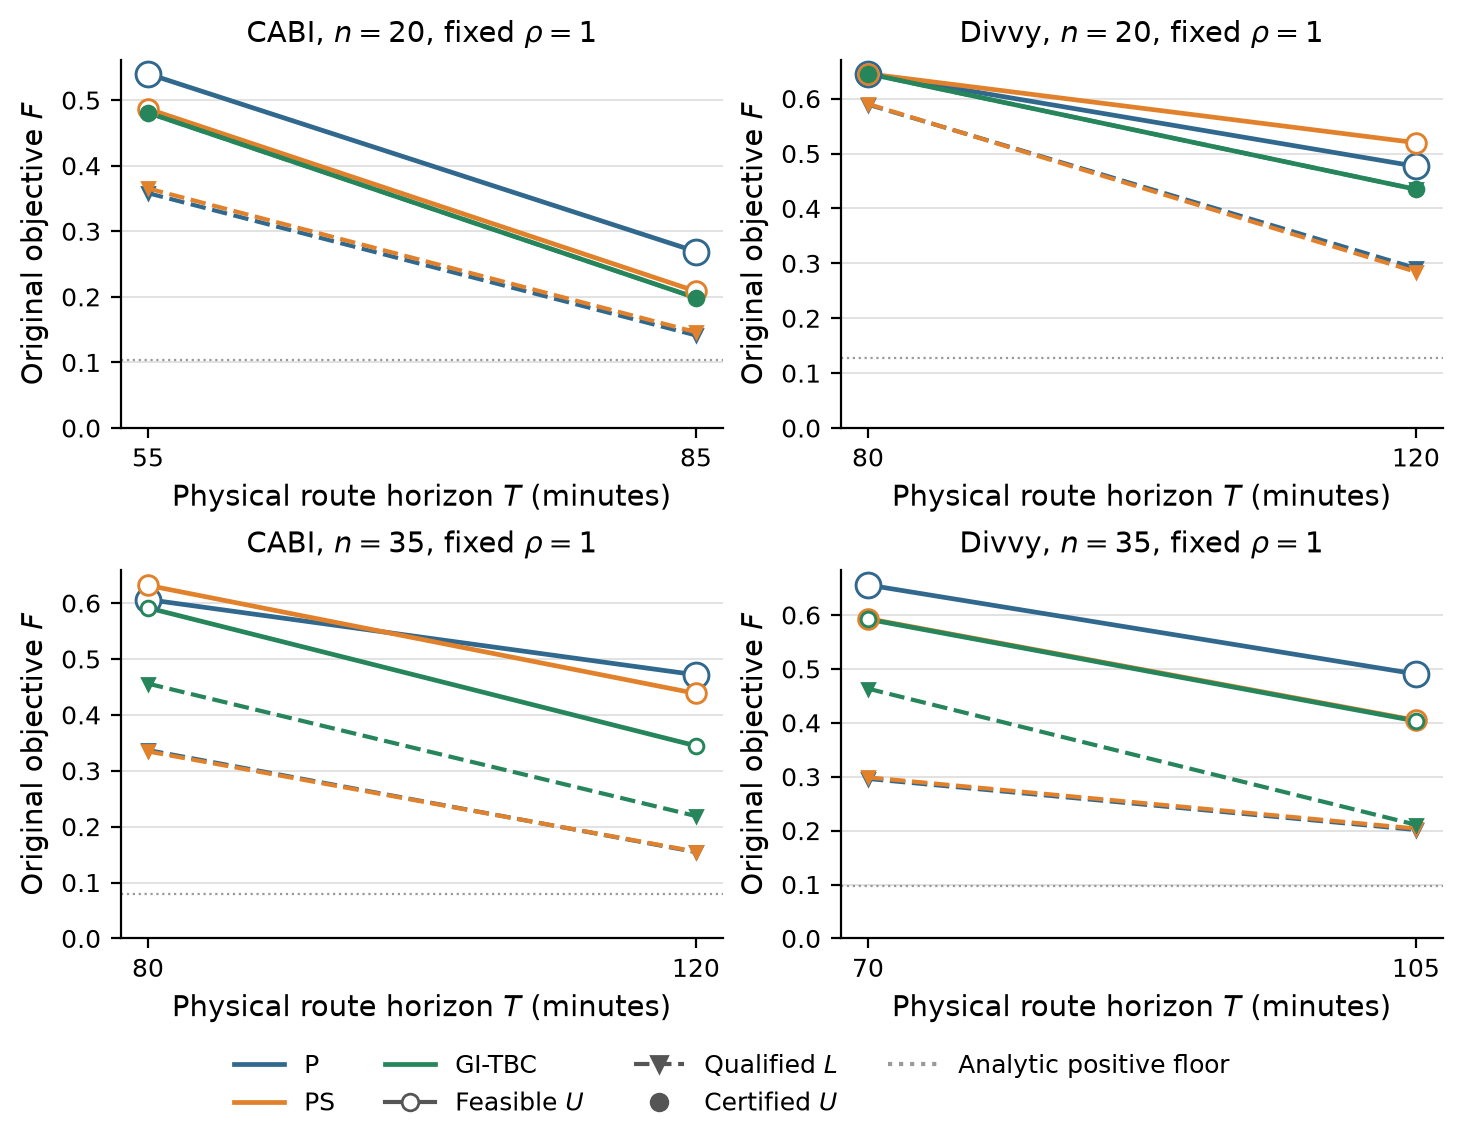
\includegraphics[keepaspectratio,alt={Original-objective endpoints at the two physical horizons. Solid lines join feasible U circles; dashed lines join qualified L triangles. Filled U circles denote qualified certificates, and grey dotted lines show the pre-solve positive floor. Connecting lines describe finite-budget observations, not an exact optimal-value curve.}]{figures/resource_endpoints.png}}
\caption{Original-objective endpoints at the two physical horizons.
Solid lines join feasible U circles; dashed lines join qualified L
triangles. Filled U circles denote qualified certificates, and grey
dotted lines show the pre-solve positive floor. Connecting lines
describe finite-budget observations, not an exact optimal-value curve.}
\end{figure}

\clearpage

\subsubsection{5.3 Objective weights}\label{objective-weights}

\Needspace{8\baselineskip}

\textbf{Table 6. Objective-weight evidence. (a) Sampled complete-method
outcomes; C denotes an own qualified certificate.}

{\def\LTcaptype{none} % do not increment counter
\begin{longtable}[]{@{}
  >{\raggedright\arraybackslash}p{(\linewidth - 8\tabcolsep) * \real{0.2000}}
  >{\raggedright\arraybackslash}p{(\linewidth - 8\tabcolsep) * \real{0.2000}}
  >{\raggedright\arraybackslash}p{(\linewidth - 8\tabcolsep) * \real{0.2000}}
  >{\raggedright\arraybackslash}p{(\linewidth - 8\tabcolsep) * \real{0.2000}}
  >{\raggedright\arraybackslash}p{(\linewidth - 8\tabcolsep) * \real{0.2000}}@{}}
\toprule\noalign{}
\begin{minipage}[b]{\linewidth}\raggedright
Physical configuration
\end{minipage} & \begin{minipage}[b]{\linewidth}\raggedright
\(\rho\)
\end{minipage} & \begin{minipage}[b]{\linewidth}\raggedright
P: U / L
\end{minipage} & \begin{minipage}[b]{\linewidth}\raggedright
PS: U / L
\end{minipage} & \begin{minipage}[b]{\linewidth}\raggedright
GI-TBC: U / L
\end{minipage} \\
\midrule\noalign{}
\endhead
\bottomrule\noalign{}
\endlastfoot
R-B20-S-T1 & 0.5 & 0.380389 /0.229542 (open) & 0.347458 /0.240479 (open)
& 0.347458 /0.331864 (open) \\
R-B20-S-T1 & 1 & 0.540085 /0.358158 (open) & 0.486639 /0.365324 (open) &
0.480735 /0.480735 (C) \\
R-B20-S-T1 & 2 & 0.756988 /0.610312 (open) & 0.744646 /0.616106 (open) &
0.744646 /0.744646 (C) \\
R-X35-S-T2 & 0.5 & 0.260978 /0.108223 (open) & 0.257631 /0.108019 (open)
& 0.255825 /0.122332 (open) \\
R-X35-S-T2 & 1 & 0.490517 /0.201288 (open) & 0.404567 /0.203817 (open) &
0.403272 /0.210887 (open) \\
R-X35-S-T2 & 2 & 0.620443 /0.36178 (open) & 0.611892 /0.363572 (open) &
0.524553 /0.388438 (open) \\
\end{longtable}
}

The sampled comparisons retain different search outcomes: B certifies
R-B20-S-T1 at \(\rho=1,2\), while all methods remain open at
\(\rho=.5\); all three methods remain open at every tested R-X35-S-T2
weight. The table reports each original run's own U/L. Cross-weight
information is used only for the following offline analysis.

We reconstruct every available complete fleet from the two
configurations above and from the earlier K-15-S and UC-B20-B weight
study: 32 run records, with all method/Seed owners retained. Routes,
nonzero one-way operations, stock balance, empty departure, load
prefixes, loaded returns and unloading time are independently checked.
Each family has identical physical data and normalized station weights.
True Gini and weighted penalty are recomputed from the full inventories
and actual loaded weights; rounded table components are not used to
manufacture fleets or certificates.

For a fixed family, put \(p(x)=P(x)/\Omega\) and

\[
v(\rho)=\min_{x\in\mathcal F}\{G(x)+\rho p(x)\},\qquad
U_{\mathcal A}(\rho)=\min_{x\in\mathcal A}\{G(x)+\rho p(x)\}.
\]

The archive \(\mathcal A\) contains only verified physical fleets. Thus
\(U_{\mathcal A}\) is an upper bound, not the algorithm's result at
unrun weights. The value \(v\) is concave as an infimum of affine
functions. For qualified global \(L_a\le v(\rho_a)\),
\(L_b\le v(\rho_b)\), \(\rho_a<\rho_b\), concavity gives the lower chord

\[
v(\rho)\ge\frac{\rho_b-\rho}{\rho_b-\rho_a}L_a+
\frac{\rho-\rho_a}{\rho_b-\rho_a}L_b,\qquad \rho\in[\rho_a,\rho_b].
\]

Let \(L_C\) be the maximum of applicable chords. A repeated actual
coordinate uses the greatest qualified lower and contributes no
zero-length chord. Chords are never extrapolated. These standard
parametric-optimization facts yield
\(0\le U_{\mathcal A}(\rho)-v(\rho)\le U_{\mathcal A}(\rho)-L_C(\rho)\).
We calculate the worst bound over the entire covered interval from all
true affine-line intersections, active-chord intersections and domain
endpoints using rational arithmetic. No dense grid or new solver is
used. Actual binary64 lambda/weight coordinates are retained, including
small differences from displayed .5/1/2. The numerical guards are those
stated with Table 5.

\Needspace{14\baselineskip}

\textbf{Table 6, panel (b). Continuous-weight quality guarantees from
the complete fleet archive.} Ranges below are display coordinates; the
machine-readable data preserve exact loaded coordinates. Regret bounds
are rounded upward.

{\def\LTcaptype{none} % do not increment counter
\begin{longtable}[]{@{}
  >{\raggedright\arraybackslash}p{(\linewidth - 8\tabcolsep) * \real{0.2000}}
  >{\raggedright\arraybackslash}p{(\linewidth - 8\tabcolsep) * \real{0.2000}}
  >{\raggedright\arraybackslash}p{(\linewidth - 8\tabcolsep) * \real{0.2000}}
  >{\raggedright\arraybackslash}p{(\linewidth - 8\tabcolsep) * \real{0.2000}}
  >{\raggedright\arraybackslash}p{(\linewidth - 8\tabcolsep) * \real{0.2000}}@{}}
\toprule\noalign{}
\begin{minipage}[b]{\linewidth}\raggedright
Fixed physical family
\end{minipage} & \begin{minipage}[b]{\linewidth}\raggedright
Covered rho range
\end{minipage} & \begin{minipage}[b]{\linewidth}\raggedright
Runs / distinct G,p lines
\end{minipage} & \begin{minipage}[b]{\linewidth}\raggedright
Supported archive lines
\end{minipage} & \begin{minipage}[b]{\linewidth}\raggedright
Worst absolute regret bound
\end{minipage} \\
\midrule\noalign{}
\endhead
\bottomrule\noalign{}
\endlastfoot
K-15-S & {[}0.710502825, 2.8420113{]} & 8 / 3 & 3 & 0.002356282 \\
UC-B20-B & {[}0.88725, 3.549{]} & 6 / 1 & 1 & 0.000000100002 \\
R-B20-S-T1 & {[}0.5, 2{]} & 9 / 7 & 3 & 0.015594269 \\
R-X35-S-T2 & {[}0.5, 2{]} & 9 / 9 & 1 & 0.136115162 \\
\end{longtable}
}

UC-B20-B has the same component line across the full historical range,
with an essentially numerical-width bound for one fixed fleet. K-15-S
exhibits three supported component choices; the largest archive regret
bound occurs at \(\rho\approx1.217804157\), between sampled weights.
R-B20-S-T1 has component tradeoffs but a wider low-weight search gap.
R-X35-S-T2 has one archive line supported throughout, while its proof
band remains wide. Dominated fleets and their owners remain in the
archive. Stability among known fleets does not prove a complete optimal
frontier.

The R-X35-S-T2 fleet found at the higher sampled weight improves both
components of the original unit-weight B incumbent. Re-evaluated at its
actual original rho coordinate, its feasible objective is 0.3365058165
instead of 0.4032719989, a known improvement of 0.06676618239. The old
U, discovery time and certificate status are unchanged. This offline
deficit diagnosis is not injected into the C166/B comparison's startup
or treated as production acceleration.

\begin{figure}
\centering
\pandocbounded{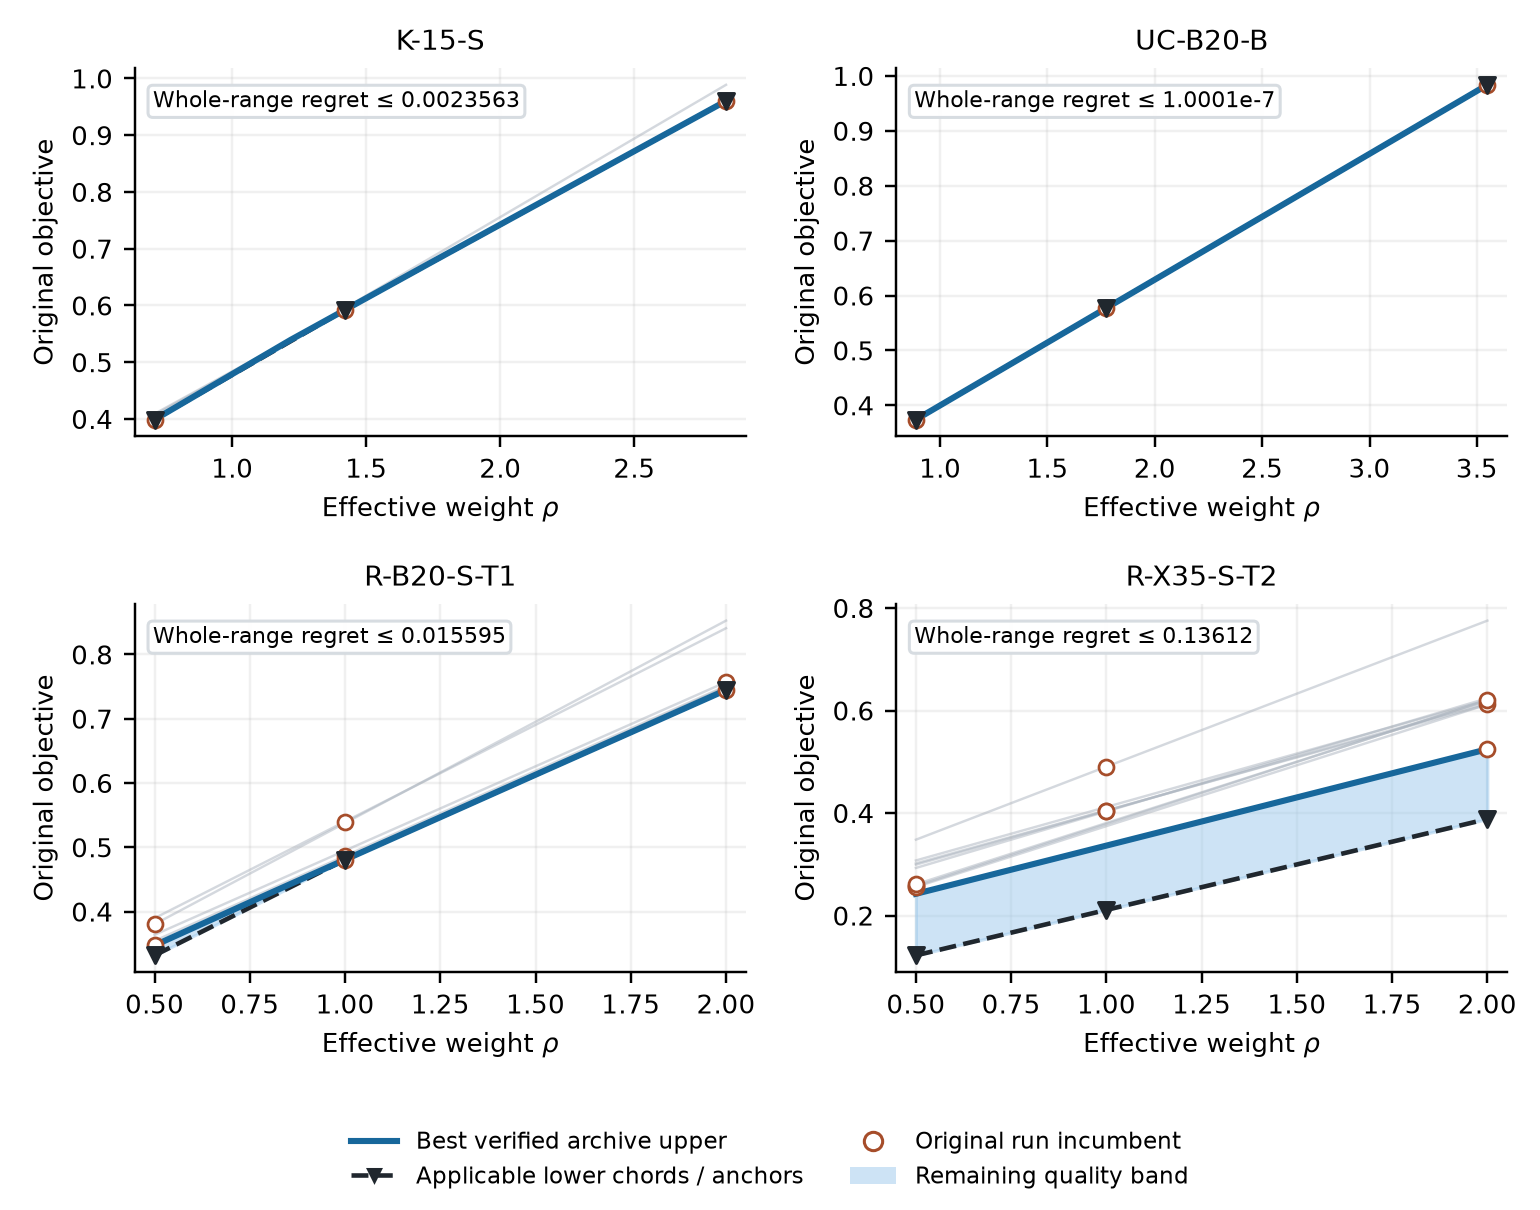
\includegraphics[keepaspectratio,alt={Certified continuous-weight bands for four fixed physical families. Blue is the best verified archive objective; black dashed chords are applicable qualified lower bounds; shading is the remaining quality band. Pale lines retain other feasible component choices, circles mark original run incumbents, and triangles mark qualified lower anchors. These are upper/lower bounds, not a known exact optimum curve.}]{figures/parameter_quality_bands.png}}
\caption{Certified continuous-weight bands for four fixed physical
families. Blue is the best verified archive objective; black dashed
chords are applicable qualified lower bounds; shading is the remaining
quality band. Pale lines retain other feasible component choices,
circles mark original run incumbents, and triangles mark qualified lower
anchors. These are upper/lower bounds, not a known exact optimum curve.}
\end{figure}

\clearpage

\subsubsection{5.4 Limited preselected second
Seed}\label{limited-preselected-second-seed}

\Needspace{8\baselineskip}

\textbf{Table 7. Certificates in the four preselected second-Seed
configurations.}

{\def\LTcaptype{none} % do not increment counter
\begin{longtable}[]{@{}lll@{}}
\toprule\noalign{}
Method & Selected Seed 0 certificates /4 & Seed 1 certificates /4 \\
\midrule\noalign{}
\endhead
\bottomrule\noalign{}
\endlastfoot
P & 1 & 1 \\
PS & 1 & 1 \\
GI-TBC & 3 & 3 \\
\end{longtable}
}

These four configurations were selected before the current results.
Their Seed 1 observations remain distinct from the full main Seed 0
panel and do not replace an unfavorable first observation. Same Seed is
a common setting for different models, not a shared random trajectory,
and two Seeds do not estimate a runtime distribution. Complete H remains
part of the defined algorithm configuration with its own fixed seed; the
AM/mechanism repeat blocks use the corresponding actual Seed 1
baselines.

K-15-S retains the same certificate pattern in the limited repeat: only
GI-TBC certifies, in 112.769 / 115.444 s at Seed 0 / Seed 1, a
nonmaterial complete-cost difference under the declared rule. All six
runs attain the same verified feasible objective, but each compact run
retains its own open proof status. Finite dual progress is less stable
in direction: Seed 0 cold P / paid-start PS end at L=0.527663/0.520583,
whereas Seed 1 ends at 0.529115/0.53228. Thus the compact dual ordering
reverses even while feasible objectives and this role-specific
certificate pattern agree. This finite observation does not establish a
distribution or an eventual proof-time ranking.

UC-B20-B also retains its certificate pattern, with all three methods
certifying at both Seeds. GI-TBC takes 4.14897/4.0999 s and cold P
315.403/314.513 s, respectively; their cross-Seed differences are below
the substantive rule. Paid-start PS changes from 236.091 to 125.391 s.
This descriptive change exceeds that rule while the GI-TBC advantage
over both compact controls persists in this role. Complete own H and
matched within-Seed trace/fleet identities are retained; unchanged
certification status does not make every complete runtime stable. Two
Seeds still supply finite checks rather than a distribution or a
best-Seed selection.

R-B20-S-T1 preserves own certification only for GI-TBC, whose
certificate cost changes from 784.143 to 656.734 s, a substantive
descriptive shift under the stated rule. At Seed 1, paid-start PS
reaches the same feasible U=0.480735, but retains its own lower endpoint
0.367482 and remains open. Cold P improves its feasible objective from
0.540085 to 0.493224 while its lower bound falls from 0.358158 to
0.354626. The complete-method certificate pattern therefore coexists
with material time variation and opposed cross-Seed endpoint changes.
These are finite matched observations; the Seed 0 panel remains the
primary evidence, and no certificate is transferred to a compact run.

K-35-U remains open for every method at both Seeds. At Seed 1, GI-TBC
has U/L=0.668358/0.55478, compared with P 0.758852/0.330574 and PS
0.712648/0.335095. GI-TBC improves both endpoints over both controls
within Seed 1, whereas Seed 0 retains the better P feasible objective
and stronger GI-TBC lower bound. GI-TBC also improves its own U from
0.692854 to 0.668358 across Seeds while L falls from 0.565766 to
0.55478. A smaller signed gap therefore does not make both of its own
endpoints better. The compact comparison reverses in both endpoints: P
is better than PS at Seed 0, while PS is better than P at Seed 1. No
open certificate time is supplied, and the adverse Seed 0 observations
are retained.

\subsubsection{5.5 Archived-source cohort and within-input Seed
confirmation}\label{archived-source-cohort-and-within-input-seed-confirmation}

The six-configuration cohort was generated once from a prospectively
frozen recipe using three archived sources, two sizes and three
compact/three regional selections. All configurations and all 18 Seed0
B/E+/P commands were sealed before the formal comparison;
balanced/surplus and shortage selections were retained regardless of
difficulty or inventory-floor value. Synthetic inventories, targets and
weights are not observed demand. This supplies finite configuration
coverage rather than new-city or IID validation. These same six
configurations are now exposed when used for additional solver-Seed
confirmation.

Each configuration has independently paid B, E+ and cold P runs under
one common PE/DLL, original physical T, actual lambda and cap. The n20
cap is 1200 s and n35 cap 2400 s, including startup and helper. P has
NumStart=0; B/E+ each execute their own H. Original complete fleets are
independently recomputed. Qualified proof endpoints and the inherited
signed/near-zero certificate policy determine state. OPEN cap values are
not certificate times.

\textbf{Table 8. Historical Seed0 configuration confirmation, separate
from the earlier panels.} Each entry is state, physical U / qualified
proof L, then paid T\_\allowbreak{}cert for CERT (seconds). Full binary64 values,
verification costs, Work/nodes and source identities are in the
supplement.

{\def\LTcaptype{none} % do not increment counter
\begin{longtable}[]{@{}
  >{\raggedright\arraybackslash}p{(\linewidth - 6\tabcolsep) * \real{0.2500}}
  >{\raggedright\arraybackslash}p{(\linewidth - 6\tabcolsep) * \real{0.2500}}
  >{\raggedright\arraybackslash}p{(\linewidth - 6\tabcolsep) * \real{0.2500}}
  >{\raggedright\arraybackslash}p{(\linewidth - 6\tabcolsep) * \real{0.2500}}@{}}
\toprule\noalign{}
\begin{minipage}[b]{\linewidth}\raggedright
Configuration
\end{minipage} & \begin{minipage}[b]{\linewidth}\raggedright
B
\end{minipage} & \begin{minipage}[b]{\linewidth}\raggedright
E+
\end{minipage} & \begin{minipage}[b]{\linewidth}\raggedright
P
\end{minipage} \\
\midrule\noalign{}
\endhead
\bottomrule\noalign{}
\endlastfoot
C20-S & CERT; 0.1912806 / 0.1912806; T\_\allowbreak{}cert=199.7794 & CERT; 0.1912806
/ 0.1912806; T\_\allowbreak{}cert=225.8837 & OPEN; 0.1912806 / 0.1602342 \\
B20-B & CERT; 0.4232322 / 0.4232322; T\_\allowbreak{}cert=5.058292 & CERT; 0.4232322
/ 0.4232322; T\_\allowbreak{}cert=6.756587 & CERT; 0.4232322 / 0.4232322;
T\_\allowbreak{}cert=235.8555 \\
X20-S & CERT; 0.4477476 / 0.4477476; T\_\allowbreak{}cert=119.7494 & CERT; 0.4477476
/ 0.4477476; T\_\allowbreak{}cert=125.9267 & OPEN; 0.4609478 / 0.2616497 \\
C35-U & OPEN; 0.1295664 / 0.0198375 & OPEN; 0.1295664 / 0.0198375 &
OPEN; 0.09331934 / 0.008286772 \\
B35-S & OPEN; 0.1942903 / 0.120234 & OPEN; 0.1942903 / 0.120234 & OPEN;
0.249253 / 0.1139794 \\
X35-S & OPEN; 0.4574753 / 0.3949883 & OPEN; 0.4574753 / 0.4231995 &
OPEN; 0.5415307 / 0.3629714 \\
\end{longtable}
}

Both B and E+ certify 3/6 configurations, versus cold P 1/6. Their
physical U agree on all six; E+ raises only X35's final qualified L,
from .3949882559151472 to .42319954961578576 at U=.45747531701601785.
The original relative gap falls from 13.659110945800548\% to
7.492375244155952\%, without a new certificate or primal improvement.
Its slightly lower raw search L=.39492875817006656 distinguishes the
independent proof contribution from AM/Native search progress. B/P tests
the integrated main method, while E+/B isolates the complete enhancement
comparison; no per-configuration best-of-B/E+ result is formed.

For the three joint-CERT E+/B pairs, E+ adds about 26.10 s on C20, 1.70
s on B20 and 6.18 s on X20; the ratios are 1.13067, 1.33574 and 1.05159.
Only C20 meets the declared substantive scale
\(\max\{10\text{ s},.1\times\text{faster time}\}\). The other two
numerical increases remain nonmaterial. The helper and verification
ledgers in the supplement retain their full costs without adding nested
helper time twice. Uniform E+ is a reasonable alternative when its
stronger X35 proof endpoint is prioritized. Choosing B as the main paper
method balances certificate count, paid time and both endpoints; it is
not a dominance theorem.

B and E+ each have lower U than P on three configurations, higher U on
C35-U, and equivalent U on two. Their proof L are higher on five
configurations and equivalent at the frozen numerical scale on B20. In
particular, C35-U retains P's better U=.09331934374779818 against B/E+'s
.12956638965196035, together with the opposite proof direction. The B/P
and E+/P joint-CERT intersections each contain only B20 (1/6); their
conditional time ratios supply no full-panel speedup. Every OPEN
endpoint and paid cost remains included, and a single Seed does not
estimate a runtime distribution.

C20, B20 and X20 finish with search L above their qualified inventory
value uppers. C35's numerically near-zero inventory result is not an
exact-zero physical proof. The capacity-limited B35/X35 inventory widths
remain .014387103336740467/.02295563610060769. B35's floor is below
final search L while its inventory upper is above it; X35's floor
improves the final proof but its price remains unresolved. Earlier
near-tight same-domain inventory results therefore do not bound these
two remainders.

The proof-only helper adds no floor to Native rows or raw AM. Its
separate return-time/floor/search-L ledger distinguishes dominated
inventory values, zero optima, rejected sources and unresolved prices. A
tighter inventory proof source supplies neither a physical incumbent nor
an automatic complete-method benefit. These E+ observations retain their
one-Seed scope.

\paragraph{Finite solver-Seed confirmation on the exposed
cohort}\label{finite-solver-seed-confirmation-on-the-exposed-cohort}

The same six inputs were subsequently registered together for Gurobi
Seeds1/2, giving 24 additional B/P runs and twelve new paired
comparisons. Historical Seed0 qualifies under the same input, physical,
method, executable, numerical and paid-clock contracts, with matching
documented runtime observations. Each new run starts a fresh lifecycle;
B recomputes and pays its own H with seed20260626. These are six
mathematical inputs with three within-input observations each, rather
than eighteen independent new inputs. No best Seed, cross-Seed
certificate, additional method or outcome-dependent stop is used.

\textbf{Table 9. Within-input paired differences in Seed order 0/1/2.}
Seed 0 is historical; Seeds 1/2 are the subsequent confirmation
observations. ΔU=B−P is favorable to B when negative; ΔL=B−P is
favorable when positive. Values within the frozen 1e-7 equivalence scale
are displayed as 0. Full individual U/L, raw search bounds, paid costs,
medians/ranges and binary64 values remain in the supplement.

{\def\LTcaptype{none} % do not increment counter
\begin{longtable}[]{@{}
  >{\raggedright\arraybackslash}p{(\linewidth - 8\tabcolsep) * \real{0.2000}}
  >{\raggedright\arraybackslash}p{(\linewidth - 8\tabcolsep) * \real{0.2000}}
  >{\raggedright\arraybackslash}p{(\linewidth - 8\tabcolsep) * \real{0.2000}}
  >{\raggedright\arraybackslash}p{(\linewidth - 8\tabcolsep) * \real{0.2000}}
  >{\raggedright\arraybackslash}p{(\linewidth - 8\tabcolsep) * \real{0.2000}}@{}}
\toprule\noalign{}
\begin{minipage}[b]{\linewidth}\raggedright
Configuration
\end{minipage} & \begin{minipage}[b]{\linewidth}\raggedright
B CERT /3
\end{minipage} & \begin{minipage}[b]{\linewidth}\raggedright
P CERT /3
\end{minipage} & \begin{minipage}[b]{\linewidth}\raggedright
ΔU: S0 / S1 / S2
\end{minipage} & \begin{minipage}[b]{\linewidth}\raggedright
ΔL: S0 / S1 / S2
\end{minipage} \\
\midrule\noalign{}
\endhead
\bottomrule\noalign{}
\endlastfoot
C20-S & 3 & 0 & 0 / 0 / -0.05927393 & 0.03104638 / 0.03369846 /
0.03941158 \\
B20-B & 3 & 3 & 0 / 0 / 0 & 0 / 0 / 0 \\
X20-S & 3 & 0 & -0.01320014 / -0.01721348 / -0.01320014 & 0.186098 /
0.1948245 / 0.1974955 \\
C35-U & 0 & 0 & 0.03624705 / -0.05019445 / -0.03868052 & 0.01155073 /
0.01347433 / 0.009334378 \\
B35-S & 0 & 0 & -0.0549627 / -0.101716 / -0.13296 & 0.006254594 /
0.004661458 / 0.004752414 \\
X35-S & 0 & 0 & -0.08405536 / -0.06065283 / -0.06178785 & 0.03201682 /
0.04660159 / 0.04442013 \\
\end{longtable}
}

At each Seed, B certifies 3/6 inputs and P 1/6. The three n20 B
certificate patterns persist, while cold P certifies only B20. B35 and
X35 retain lower B U and higher B L at every Seed, but all eighteen n35
method observations remain OPEN. C35's primal ordering reverses: P is
better at Seed0, whereas B is better at Seeds1/2. B's C35 L remains
higher at all three Seeds. These input-specific consistencies do not
establish a general success probability or a structural cause of the
observed differences.

\textbf{Table 10. Paid n20 certificate times, seconds.} A dash means
OPEN, without an imputed convergence time.

{\def\LTcaptype{none} % do not increment counter
\begin{longtable}[]{@{}
  >{\raggedright\arraybackslash}p{(\linewidth - 4\tabcolsep) * \real{0.3333}}
  >{\raggedright\arraybackslash}p{(\linewidth - 4\tabcolsep) * \real{0.3333}}
  >{\raggedright\arraybackslash}p{(\linewidth - 4\tabcolsep) * \real{0.3333}}@{}}
\toprule\noalign{}
\begin{minipage}[b]{\linewidth}\raggedright
Configuration
\end{minipage} & \begin{minipage}[b]{\linewidth}\raggedright
B T\_\allowbreak{}cert: S0 / S1 / S2
\end{minipage} & \begin{minipage}[b]{\linewidth}\raggedright
P T\_\allowbreak{}cert: S0 / S1 / S2
\end{minipage} \\
\midrule\noalign{}
\endhead
\bottomrule\noalign{}
\endlastfoot
C20-S & 199.7794 / 354.3877 / 341.81022 & - / - / - \\
B20-B & 5.058292 / 4.963643 / 5.277053 & 235.8555 / 303.0334 /
266.8006 \\
X20-S & 119.7494 / 136.9986 / 131.8292 & - / - / - \\
\end{longtable}
}

\begin{figure}
\centering
\pandocbounded{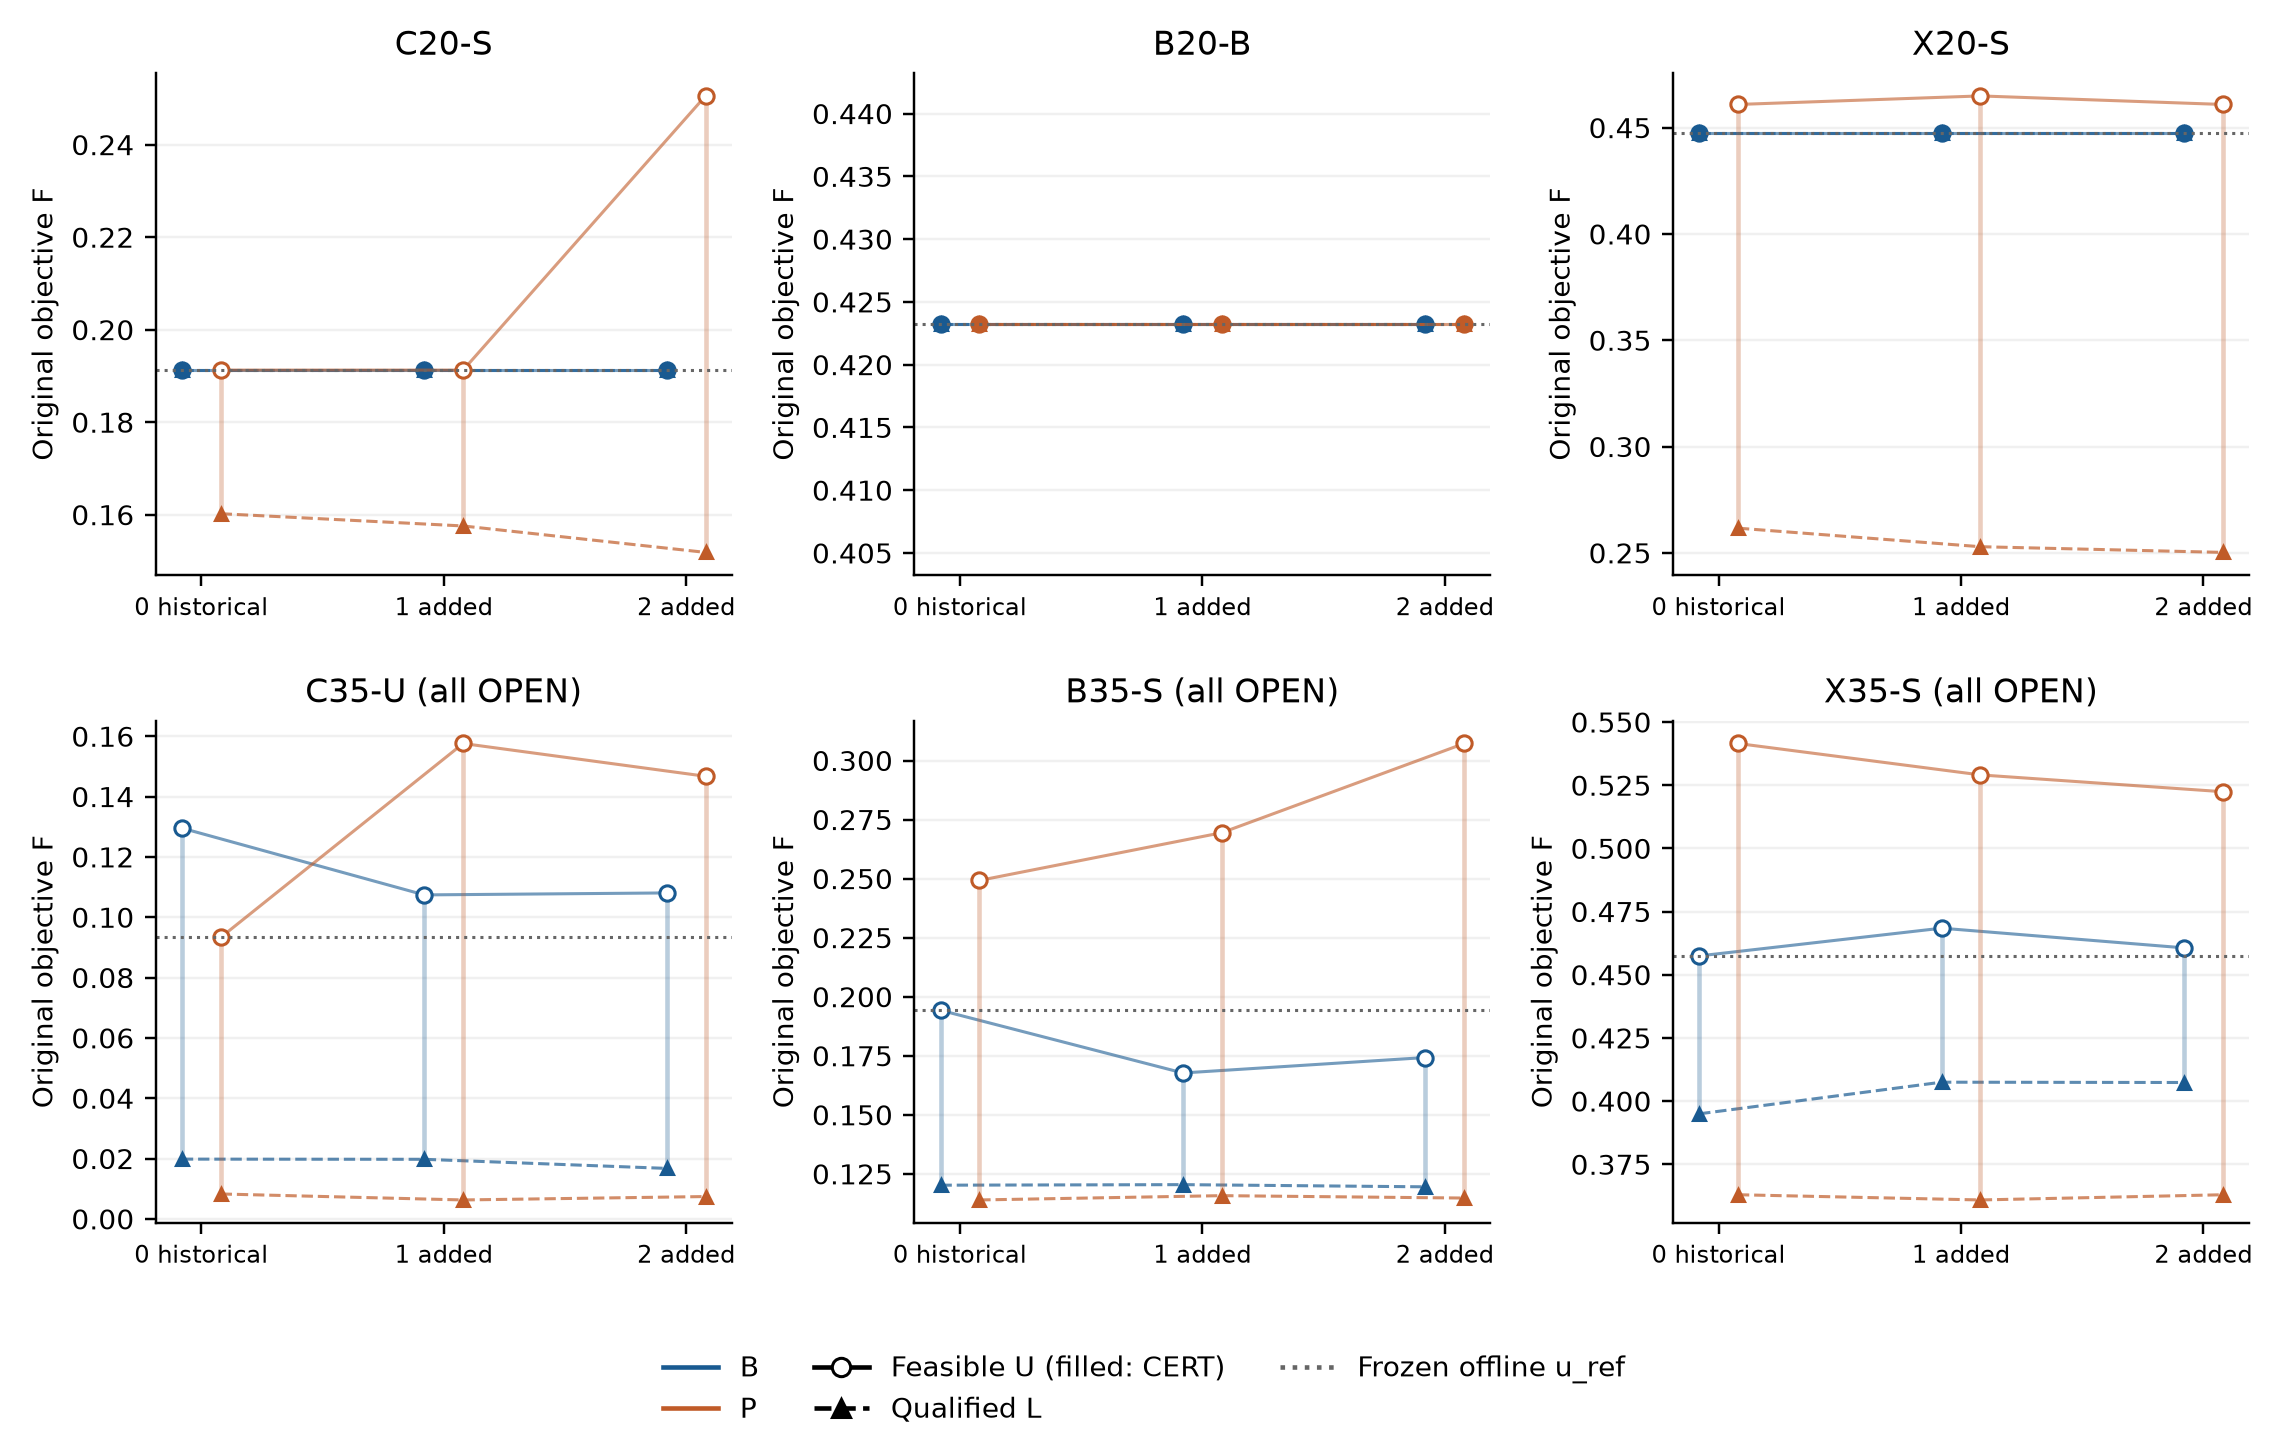
\includegraphics[keepaspectratio,alt={Three-Seed original-objective endpoints on the six archived-source inputs. Colours identify B and cold P; circles are physical U and triangles qualified L. Filled U circles denote CERT and open circles OPEN. Dotted lines mark the pre-frozen offline feasible target. Seed 0 is historical; Seeds 1/2 were added on these same exposed inputs. Lines connect repeated observations and imply neither independent inputs nor a performance distribution.}]{figures/three_seed_endpoints.png}}
\caption{Three-Seed original-objective endpoints on the six
archived-source inputs. Colours identify B and cold P; circles are
physical U and triangles qualified L. Filled U circles denote CERT and
open circles OPEN. Dotted lines mark the pre-frozen offline feasible
target. Seed 0 is historical; Seeds 1/2 were added on these same exposed
inputs. Lines connect repeated observations and imply neither
independent inputs nor a performance distribution.}
\end{figure}

Certificate-status consistency does not imply constant complete cost.
B's C20 and X20 times vary substantively across these observations under
the declared scale; its B20 spread is below 10 s, whereas P's B20 range
is 235.8555019-303.0333761 s. Within each Seed, the joint-CERT B/P
intersection contains only B20 (1/6). Its B/P time ratios at Seeds0/1/2
are .02144657385/.01637985662/.01977901536 and its signed paid
differences are −230.7972095/−298.0697328/−261.5235357 s. Each exceeds
the 10 s substantive scale in B's favor. These conditional comparisons
supply no full-panel speedup, and an OPEN budget is never treated as a
certificate time.

The uniform offline target is the better qualified Seed0 U, frozen
before any new Optimize and absent from production. B reaches the saved
target on all three observations of each n20 input and B35; on C35 it
reaches none, and on X35 only the historical Seed0 observation reaches
it. P reaches it on all three B20 observations, two C20 observations and
historical C35 Seed0, with none observed on X20/B35/X35. In particular,
B's new X35 U are both worse than its own Seed0 U while its L are
stronger, despite favorable within-Seed B/P directions. Recorded
availability intervals and censoring, not exact first-discovery times or
impossible-target claims, support these statements.

The C35 H value is .17449020363402973 at all three fixed-H-seed
lifecycles. Native improves B's U to
.12956638965196035/.10742986645444105/ .10808393649972804; P's U are
.09331934374779818/.15762431259566606/ .14676445594619023. The
historical P fleet therefore still supplies a known better feasible
point for every B run. Its advantage is not a persistent within-Seed
P-over-B ranking. Seed0's fleets differ in ownership, service amounts
and co-served relative order simultaneously; no single operator or
route-feedback benefit is isolated. The fixed unserved-station penalty
.011402553447730399 cannot exclude attaining P's target. Setting the
other visited inventories to target gives .03359254619609878, but
exceeds the saved routes' time limits and one prefix capacity. It is
neither a physical solution nor a certificate about every legal service
choice on that skeleton.

\clearpage

\subsection{6. Mechanisms, AM and stage
interpretation}\label{mechanisms-am-and-stage-interpretation}

\subsubsection{6.1 AM rule and experimental
interpretation}\label{am-rule-and-experimental-interpretation}

For finite valid child LP evidence, the actual controller uses

\[
\begin{aligned}
\Delta&=\max\{U-b,\max(\epsilon, 10^{-12})\},\\
v_j&=\operatorname{clip}_{[0,1]}((\ell_j-b)/\Delta),\qquad j=0,1,\\
\eta&=\min(v_0,v_1),\qquad
\mu=(v_0+v_1)/2,\qquad S_{\mathrm{AM}}=\eta\mu.
\end{aligned}
\]

The actual eligibility conditions, score tolerance, terminal decisions
and target continuation remain unchanged. An infeasible child invokes
logical coverage handling independently of this finite-score threshold.
Missing or invalid evidence cannot justify a split. A run without a
finite gate exposure does not test threshold sensitivity. Depth 8 and
minimum width 1e-4 are fixed. The preserved AM construction and
threshold-validation evidence in the supplement supports the default
.08; the bounded current study compares .04/.08/.16 without per-instance
selection.

The research control sets the actual first-class split threshold after
presets; the implementation mapping and readback checks are specified in
Appendix B.1. Offline replay can describe different actions at observed
states, but cannot reuse the original post-divergence trajectory as a
runtime counterfactual. The score estimates gap-normalized two-sided
bound improvement, not remaining complete proof cost.

The Seed 0 AM comparison contains eight additional positions and twelve
views after sharing the four matching default runs. The Seed 1 AM block
contains four additional positions and six views, using its two
independently measured Seed 1 defaults.

\Needspace{8\baselineskip}

\textbf{Table 11. Observed Seed 0 AM score gates, actions and complete
production cost.}

\textbf{Seed 0 main AM comparison}

{\def\LTcaptype{none} % do not increment counter
\begin{longtable}[]{@{}
  >{\raggedright\arraybackslash}p{(\linewidth - 8\tabcolsep) * \real{0.2000}}
  >{\raggedright\arraybackslash}p{(\linewidth - 8\tabcolsep) * \real{0.2000}}
  >{\raggedright\arraybackslash}p{(\linewidth - 8\tabcolsep) * \real{0.2000}}
  >{\raggedright\arraybackslash}p{(\linewidth - 8\tabcolsep) * \real{0.2000}}
  >{\raggedright\arraybackslash}p{(\linewidth - 8\tabcolsep) * \real{0.2000}}@{}}
\toprule\noalign{}
\begin{minipage}[b]{\linewidth}\raggedright
Role
\end{minipage} & \begin{minipage}[b]{\linewidth}\raggedright
\(\tau_{\mathrm{AM}}\)
\end{minipage} & \begin{minipage}[b]{\linewidth}\raggedright
Max gate score
\end{minipage} & \begin{minipage}[b]{\linewidth}\raggedright
Actions
\end{minipage} & \begin{minipage}[b]{\linewidth}\raggedright
Production (s)
\end{minipage} \\
\midrule\noalign{}
\endhead
\bottomrule\noalign{}
\endlastfoot
K-15-S & 0.04 & 0.000356687 & native-target:1, exact-close:1 &
113.062 \\
K-15-S & 0.08 & 0.000356687 & native-target:1, exact-close:1 &
112.769 \\
K-15-S & 0.16 & 0.000356687 & native-target:1, exact-close:1 &
113.315 \\
UC-B20-B & 0.04 & 0.00031863 & split:3, native-target:1, exact-close:1 &
4.21966 \\
UC-B20-B & 0.08 & 0.00031863 & split:3, native-target:1, exact-close:1 &
4.14897 \\
UC-B20-B & 0.16 & 0.00031863 & split:3, native-target:1, exact-close:1 &
4.08117 \\
K-20-S & 0.04 & 0.000478466 & native-target:1, exact-close:1 &
1172.26 \\
K-20-S & 0.08 & 0.000478466 & native-target:1, exact-close:1 &
1172.19 \\
K-20-S & 0.16 & 0.000478466 & native-target:1, exact-close:1 &
1172.26 \\
K-35-U & 0.04 & n/a & exact-close:1 & 2371.02 \\
K-35-U & 0.08 & n/a & exact-close:1 & 2371.15 \\
K-35-U & 0.16 & n/a & exact-close:1 & 2371.03 \\
\end{longtable}
}

Scores in this table summarize finite score gates only; all-child and
finite-score ledgers are joined by decision sequence. Separate classes
retain no-strict-improvement terminal, logical one/both-child
infeasibility and other actions, including runs without a child decision
exposure. Logical infeasibility has no finite score/margin and is
independent of tau. Different thresholds need not create different
actions, and no split was forced for table coverage.

K-15-S illustrates finite threshold exposure with a wide negative
margin. Each Seed 0 run has one finite gate with normalized score
0.000356687; tolerance-adjusted margins at tau=.04/.08/.16 are
-0.0396431 / -0.0796431 / -0.159643. All select native-target, followed
by a separately classified no-strict-improvement exact-close terminal.
All three qualify certificates in 113.062 / 112.769 / 113.315 s,
respectively; their 0.545396 s spread is below the declared
substantive-difference rule. This finite comparison reports the three
actual complete runs and their observed gates; it does not establish
sensitivity on other configurations.

UC-B20-B separates logical splitting from the finite score test. Each
threshold run records three one-child-infeasible splits with no finite
score or margin; those actions are independent of tau. The subsequent
finite gate has score 0.00031863 and selects native-target at all three
thresholds. Qualified certificate times are 4.21966 / 4.14897 / 4.08117
s in the same threshold order, with no substantive time difference. The
split counts therefore do not establish that a finite AM score crossed a
threshold.

All three K-20-S runs remain open at U=0.716807, with qualified L in
{[}0.705356,0.705386{]}. The observed finite gate score is 0.000478466,
below the tested thresholds. The later exact-close label names a
scheduled exact solve; it does not mean that a qualified certificate was
completed. These capped endpoints and unchanged finite-gate choices do
not establish a general threshold ranking.

K-35-U reaches a finite no-strict-child-improvement terminal before a
threshold comparison in each run. The paired child observations are
present, but no finite score gate is exposed; the near-zero terminal
score is not counted as a threshold test. All three remain open at
U=0.692854, with L in {[}0.565766,0.566106{]}. This is distinct from
both a logical-infeasibility split and a run with no recorded child
decision.

Each tested threshold therefore yields two qualified certificates among
the same four Seed 0 roles. The observed finite gates of K-15-S, K-20-S
and UC-B20-B remain well below the smallest tested threshold; K-35-U
stops at the separate no-strict-improvement test. These finite
observations provide no basis for replacing the accepted
\(\tau_{\mathrm{AM}}=.08\), while leaving sensitivity at unvisited
states outside the claim. The limited Seed 1 checks remain separately
identified.

The limited Seed 1 AM repeat preserves these reached action classes on
both selected roles: one finite native-target gate and one no-strict
terminal, plus three logical splits on UC-B20-B. All six observations
certify, with no substantive within-role time difference across the
three thresholds. Their finite scores remain below .04 with negative
margins; the repeat does not test unvisited near-threshold states.

Across the eighteen AM views, all 51 recorded eligibility evaluations
are reconstructible and none rejects depth 8 or width 1e-4. Across all
58 current outer-controller runs, the 125 recorded evaluations likewise
contain no such rejection. These are checks of recorded guards, not
proof that no unrecorded attempt occurred or that the limits are
irrelevant elsewhere.

\subsubsection{6.2 Conditional mechanism
results}\label{conditional-mechanism-results}

The Seed 0 mechanism comparison adds sixteen positions to four shared
defaults, giving twenty views. The separately reported Seed 1 block adds
eight positions to its two actual Seed 1 defaults, giving ten views.
Root values below are observed complete LP optima, while the final
search bounds discussed in the text are different quantities.

\Needspace{8\baselineskip}

\textbf{Table 12. Observed Seed 0 initial LP optima for the conditional
mechanism controls.}

{\def\LTcaptype{none} % do not increment counter
\begin{longtable}[]{@{}llllll@{}}
\toprule\noalign{}
Role & Full & Root only & Minus A/B & Minus \(C_R\) & Minus \(C_G\) \\
\midrule\noalign{}
\endhead
\bottomrule\noalign{}
\endlastfoot
K-15-S & 0.167137 & 0.167137 & 0.167016 & 0.167137 & 0.167137 \\
UC-B20-B & 0.479076 & 0.479076 & 0.479076 & 0.479076 & 0.479076 \\
K-20-S & 0.195149 & 0.195149 & 0.193825 & 0.195149 & 0.195149 \\
K-35-U & 0.200178 & 0.200178 & 0.200178 & 0.200178 & 0.200178 \\
\end{longtable}
}

The entries are observed initial LP optima, with n/a for an unexposed
complete point. Numerical deletion attribution also requires the paired
domain, objective, cutoff and own-H checks in the supplement. Full
per-variant complete clocks, returned effort counters and limited Seed 1
observations are retained there.

All 24 paired root comparisons meet the saved
common-domain/objective/cutoff and complete-own-H conditions. A/B
deletion lowers the initial optimum by 0.000121173 on K-15-S and
0.00132415 on K-20-S. No initial objective increment above tolerance
1e-7 is observed for either resource-group or geometry/objective-group
retention on the four Seed 0 roles; the selected Seed 1 roots reproduce
these patterns. Equal initial optimal objective values do not establish
that retained rows are slack, inactive or redundant; the optimal face
and later search can change. Final lower-bound changes cannot be
relabelled as initial-root increments.

K-15-S exposes mixed conditional complete-method effects. All five
methods qualify their own certificates at the same objective. The full
method takes 112.769 s; deleting A/B or \(C_G\) takes 128.325 / 143.15
s, respectively, while deleting \(C_R\) takes 75.1064 s. Those three
differences are substantive under the declared rule, including the
deletion advantage for \(C_R\). GI-TBC-R takes 112.649 s, a nonmaterial
difference from the full method. These contrasts retain the rest of the
representation and complete own H, so their directions are conditional
rather than additive component shares.

\Needspace{8\baselineskip}

\textbf{Table 13. Conditional Seed 0 construction cost and returned
solver effort on K-15-S.}

{\def\LTcaptype{none} % do not increment counter
\begin{longtable}[]{@{}
  >{\raggedright\arraybackslash}p{(\linewidth - 10\tabcolsep) * \real{0.1667}}
  >{\raggedright\arraybackslash}p{(\linewidth - 10\tabcolsep) * \real{0.1667}}
  >{\raggedright\arraybackslash}p{(\linewidth - 10\tabcolsep) * \real{0.1667}}
  >{\raggedright\arraybackslash}p{(\linewidth - 10\tabcolsep) * \real{0.1667}}
  >{\raggedright\arraybackslash}p{(\linewidth - 10\tabcolsep) * \real{0.1667}}
  >{\raggedright\arraybackslash}p{(\linewidth - 10\tabcolsep) * \real{0.1667}}@{}}
\toprule\noalign{}
\begin{minipage}[b]{\linewidth}\raggedright
K-15-S variant
\end{minipage} & \begin{minipage}[b]{\linewidth}\raggedright
Canonical generation (s)
\end{minipage} & \begin{minipage}[b]{\linewidth}\raggedright
Explicit LP Runtime (s)
\end{minipage} & \begin{minipage}[b]{\linewidth}\raggedright
MIP Runtime sum (s)
\end{minipage} & \begin{minipage}[b]{\linewidth}\raggedright
Work sum
\end{minipage} & \begin{minipage}[b]{\linewidth}\raggedright
Native B\&B nodes sum
\end{minipage} \\
\midrule\noalign{}
\endhead
\bottomrule\noalign{}
\endlastfoot
GI-TBC & 0.414438 & 0.196 & 110.549 & 160.926 & 48701 \\
GI-TBC-R & 0.14161 & 0.0600002 & 110.807 & 160.157 & 48700 \\
minus A/B & 0.413122 & 0.16 & 126.181 & 186.183 & 55424 \\
minus \(C_R\) & 0.391302 & 0.178 & 73.048 & 109.31 & 29036 \\
minus \(C_G\) & 0.271173 & 0.169 & 141.108 & 204.7 & 68560 \\
\end{longtable}
}

The K-15-S \(C_R\) deletion reversal is accompanied by a change mainly
inside native MIP search: summed returned MIP Runtime falls from 110.549
to 73.048 s, Work from 160.926 to 109.31, and summed native B\&B nodes
from 48701 to 29036. The cumulative canonical-generation timer differs
by only 0.0231363 s. Conversely, \(C_G\) deletion reduces timed
canonical generation to 0.271173 s but increases returned MIP Runtime to
141.108 s and the complete certificate cost. These matched conditional
observations separate artifact-generation cost from the native search
that follows. They do not identify an additive causal share or a net
controller overhead. The diagnostics are nested inside production;
explicit LP counts omit internal MIP relaxations, target-MIP families
are included in the MIP sum, Work is not seconds, and node sums are
per-call native counters rather than unique nodes of the outer interval
tree. The full cost tables and actual phase statuses are retained in the
supplement.

The preselected Seed 1 mechanism repeat reverses all three K-15-S
row-deletion time directions. Full GI-TBC certifies in 115.444 s, versus
93.6997/132.475/99.6006 s after A/B, resource-group and
geometry/objective-group deletion. Each difference is substantive: A/B
and geometry/objective deletion are now faster, while resource-group
deletion is slower. The corresponding returned MIP Runtime sums are
113.257 s for full and 91.513/130.239/97.652 s after deletion. The same
initial-root pattern, independently paid H and recorded action classes
coexist with these reversed native search costs. Root-only takes 113.58
s, a nonmaterial difference. The two Seeds therefore support conditional
mixed effects, not a stable runtime ranking or an additive component
share.

All five UC-B20-B methods qualify certificates between 1.87206 and
4.91775 s. Every pairwise difference is below the ten-second absolute
floor, so this tiny case supplies no substantive complete-cost ranking.
The logical split activity reported above and the net benefit of the
whole outer package are assessed separately; visible outer actions alone
do not determine a full-method speed advantage.

The \(C_R\) result differs on K-20-S. Both runs remain open at the same
verified U=0.716807, while the full method has qualified L=0.705356
versus 0.703444 after deletion. Thus the deletion advantage in K-15-S
certificate cost coexists with better finite-budget dual progress for
the full method on K-20-S. These are final-endpoint observations at
matched complete caps; root-LP attribution additionally requires its own
matched-scope evidence.

The whole K-20-S contrast also retains an adverse endpoint for the full
controller: GI-TBC-R has the same U and final qualified L=0.706405,
above the full method's 0.705356. A/B and \(C_G\) deletion end at
L=0.704128/0.705296. All five runs remain open. These are final
qualified bounds from search under the registered budget; numerical
root-LP optima require their separate matched-scope evidence. No
certificate-time ranking follows. Row strengthening and outer scheduling
therefore have distinct conditional interpretations.

\Needspace{8\baselineskip}

\textbf{Table 14. Opposed Seed 0 open endpoints in the K-35-U mechanism
panel.}

{\def\LTcaptype{none} % do not increment counter
\begin{longtable}[]{@{}llll@{}}
\toprule\noalign{}
K-35-U variant & Own feasible U & Qualified final L & Status \\
\midrule\noalign{}
\endhead
\bottomrule\noalign{}
\endlastfoot
GI-TBC & 0.692854 & 0.565766 & open \\
GI-TBC-R & 0.692854 & 0.566106 & open \\
minus A/B & 0.654639 & 0.564355 & open \\
minus \(C_R\) & 0.689763 & 0.536996 & open \\
minus \(C_G\) & 0.666262 & 0.55098 & open \\
\end{longtable}
}

K-35-U exposes an opposed-endpoint result for \(C_G\) deletion. The full
method reports U/L=0.692854/0.565766, versus 0.666262/0.55098 after
deletion. The deleted model finds a better feasible objective, while the
full method retains the stronger qualified final lower bound. A smaller
signed gap after deletion therefore does not establish endpoint
dominance. Both ledgers record one no-strict-improvement exact-close
action under the same outer policy; the native searches remain separate
and both runs remain open. No certificate-time comparison is assigned.

A/B deletion also has opposed endpoints on K-35-U: its verified own
U/L=0.654639/0.564355 improves the feasible objective by 0.0382155,
while the full method retains L higher by 0.00141073. Both runs remain
open. Thus the full-method certificate advantage of A/B on K-15-S and
its higher final bound on K-20-S coexist with a better K-35-U feasible
objective after deletion. A smaller deletion gap does not combine these
distinct endpoint directions into dominance, and no instance-specific
setting is selected.

\(C_R\) deletion has U/L=0.689763/0.536996 on this larger role. All
three row-group deletions therefore improve the saved feasible objective
while weakening the qualified final lower endpoint relative to the full
formulation. This repeated within-role primal/dual opposition is
retained alongside the easier certificate-cost advantages and the K-15-S
\(C_R\) reversal. It does not justify an instance-specific setting or a
complete-proof-time ordering.

The legal root-only comparison also retains a higher final lower
endpoint on K-35-U: GI-TBC-R reports U/L=0.692854/0.566106, at the same
U as the full method and a final L higher by 0.000340054. Both runs
remain open under the matched complete cap. Together with K-20-S, these
selected hard-role observations show no full-controller endpoint
advantage over root-only at the saved Seed 0 endpoints. They do not
compare initial root-LP optima or establish an eventual proof-time
ordering; the remaining mechanism and limited Seed 1 findings retain
their separate scopes.

Across these four preselected Seed 0 roles, no substantive
full-over-root certificate-cost advantage is observed: the two easier
roles certify with nonmaterial differences, while both harder roles
remain open and root-only has the same U with slightly higher final L.
The strengthened root already suffices for the two easier certificates
in this panel. Thus visible outer activity and the strong integrated
GI-TBC results relative to compact controls do not assign a separate
incremental speed advantage to the outer package here. The accepted
post-R130 attribution history remains relevant with its own version and
cases; the current limited Seed 1 repeats are reported separately.

The row-deletion controls keep the configured outer policy fixed, but
can change its reached states and realized actions. On K-15-S and
K-20-S, A/B deletion records only a no-strict-improvement terminal,
while full, \(C_R\)-deleted and \(C_G\)-deleted runs each also record
one finite native-target gate. On UC-B20-B, each of the four outer
variants records three logical-infeasibility splits, one finite gate and
one terminal. On K-35-U, each records only the no-strict terminal;
root-only has no child-AM record on any role. The complete Seed 0
mechanism observations therefore contain ten finite gates, sixteen
terminals and twelve logical splits. These counts describe reached
decisions, not independent instances. Conditional formulation effects
include any induced control-path change; identical configured policy is
not identical realized scheduling or native search.

The saved initial domain/objective/cutoff and independently paid H
determine which numerical roots may be compared; the full paired report
flags their actual matches. Root values require an observed OPTIMAL LP;
n/a means no complete applicable point was exposed. The ideal deletion
relation is not a runtime theorem. Work/nodes, LP/MIP time,
model-construction cost, complete own H and outer actions accompany
these conditional contrasts; no additive allocation of total speed-up is
made. Depth 8 / minimum width 1e-4 remain fixed. Recorded eligibility
rows are joined to retained scheduler-epoch geometry; a source-rejection
reset or missing leaf makes the reconstruction unknown. Eligible child
work may stop before its ledger row, so missing records do not prove no
attempted test. The depth guard short-circuits the width check; a width
that would also reject after depth failure is not counted as another
causal trigger. Zero-width proofs without recorded guard evaluations are
not counted as width-limit triggers. Final materialized-leaf and
decision-parent/probed-child depths are distinct observations. The
full-versus-variant results and exposure limits are interpreted in the
stage decision and supplement.

\clearpage

\subsubsection{6.3 Mechanism synthesis and
boundaries}\label{mechanism-synthesis-and-boundaries}

\Needspace{8\baselineskip}

\textbf{Table 15. Mechanisms, mathematical roles, supporting evidence
and boundaries.}

{\def\LTcaptype{none} % do not increment counter
\begin{longtable}[]{@{}
  >{\raggedright\arraybackslash}p{(\linewidth - 8\tabcolsep) * \real{0.2000}}
  >{\raggedright\arraybackslash}p{(\linewidth - 8\tabcolsep) * \real{0.2000}}
  >{\raggedright\arraybackslash}p{(\linewidth - 8\tabcolsep) * \real{0.2000}}
  >{\raggedright\arraybackslash}p{(\linewidth - 8\tabcolsep) * \real{0.2000}}
  >{\raggedright\arraybackslash}p{(\linewidth - 8\tabcolsep) * \real{0.2000}}@{}}
\toprule\noalign{}
\begin{minipage}[b]{\linewidth}\raggedright
Mechanism
\end{minipage} & \begin{minipage}[b]{\linewidth}\raggedright
Mathematical role
\end{minipage} & \begin{minipage}[b]{\linewidth}\raggedright
Corresponding experiment
\end{minipage} & \begin{minipage}[b]{\linewidth}\raggedright
Supported conclusion
\end{minipage} & \begin{minipage}[b]{\linewidth}\raggedright
Boundary
\end{minipage} \\
\midrule\noalign{}
\endhead
\bottomrule\noalign{}
\endlastfoot
Complete own H & Constructs and checks its own feasible Start; supplies
no lower-bound proof & P/PS across main panels and four Seed 1 triplets
& PS materially wins X-35-B; P improves both endpoints on K-20-S and
R-X20-S-T2 & Startup package only; no operator or H-seed attribution \\
Outer interval controller & Preserves improving-interval coverage
through probing, targeting and exact continuation & Full/GI-TBC-R: four
Seed 0 roles, two Seed 1 repeats & No substantive certificate-cost gain
here; both hard Seed 0 roles have higher root-only final L & Reached
actions do not establish net benefit; prior versioned evidence remains
separate \\
Shared-state A/B links & Valid movement/visit equalities connect service
to inventory mixtures & A/B deletion: four Seed 0 roles, two Seed 1
repeats & Two initial LP increments; K-15-S time direction reverses
across Seeds; full K-20-S has higher final L & Core products retained;
unique one-way service preserves implicit quantity integrality \\
Resource group \(C_R\) & Ordered-supply and pair-cover/handling
inequalities strengthen necessary resource conditions & Single-group
deletion: four Seed 0 roles, two Seed 1 repeats; pair-only unchanged &
K-15-S deletion wins Seed 0 and loses Seed 1; full K-20-S has higher
final L; initial increments undetected & Valid LP tightening need not
accelerate search; no additive shares \\
Geometry/objective group \(C_G\) & Spread, centering and objective
estimators use dedicated auxiliaries & Single-group deletion: four Seed
0 roles, two Seed 1 repeats; original domains/products retained & K-15-S
time direction reverses; K-35-U deletion improves U and weakens L;
initial increments undetected & This group does not contain all fairness
structure; endpoint opposition persists \\
AM score and logic & Normalized child-bound score applies after
eligibility, validity and terminal tests & Three thresholds: four Seed 0
roles, two Seed 1 repeats & Finite scores stay below .04; logical splits
hold separately; K-35-U stops before its threshold test & Observed
unchanged actions do not prove global robustness or small proof cost \\
\end{longtable}
}

These rows summarize the observed conditional findings. The full Seed 0
and separately identified Seed 1 tables retain every selected role, and
the accompanying paired/root and cost reports determine where numerical
root attribution is actually exposed. Shared inventory-state/core
products are retained throughout the current mechanism study, so they
have no isolated runtime effect assigned here.

\subsubsection{6.4 Structural information and complete algorithm
value}\label{structural-information-and-complete-algorithm-value}

The structural experiments distinguish exclusion of a saved point,
improvement of a freely reoptimized same-scope LP, improvement of a paid
Native call, improvement of the complete own-H method, and confirmation
outside candidate development. These are different evidence levels.
Inventory-budget certificate gains, selected reciprocal-normalization
and Gini-deviation gains, and inventory-objective proof-floor increments
remain positive results. Their adverse and mixed complete outcomes limit
uniform adoption.

The physical projection, an integer resource necessary domain and an
inventory necessary domain can be ordered only with a proved common
objective/scope embedding. A continuous expression replacement does not
acquire an ordering from integer equivalence alone. The retained
four-station example has an exact \(1/4\) original-objective gap on its
fixed-positive-total slice even with the complete joint service hull. At
the loaded coefficient the inherited proof also minimizes over all legal
loaded-return totals; the physical problem is not newly restricted to
that slice. It distinguishes service compatibility from the integer
objective epigraph without needing a changing Gini denominator. The
\href{https://github.com/yifanXovo/TailoredExact/blob/de01e8fb27a954d031abac5fe99442d6c8d29d44/results/unified_exact_round133/joint_objective_gap_note.md}{fixed
four-station derivation} gives the instance, feasible mixtures and full
loaded-return lower proof. Shared-state movement/visit links strengthen
the fractional representation; they remain unnecessary as premises of
the implicit-integrality lemma.

The full-physical shared-G completion experiment illustrates this
distinction. Both saved points fail their fixed completion tests, but
free reoptimization on one domain returns the same qualified LP value;
the other gains about \(.00018725\). A projected row retains about 87\%
of that scoped increment. Removing the complete duration rows removes
the increment conditional on the remaining constraints; it does not
prove time alone sufficient or separate travel from handling. In six
complete primary-role arms the tested completion has worse U than both
fresh controls, equal proof L and no certificate. Four conditional
positions remain unstarted. The supplement retains the source
identities, row size, positive increment and adverse complete outcomes.

For one common global inventory relaxation and original physical
problem, \(L_I\le f_I^*\le U_I\) and \(f_I^*\le f_P^*\le U_P\) give

\[
 U_P-L_I=(U_P-f_P^*)+(f_P^*-f_I^*)+(f_I^*-L_I).
\]

Only the last term is controlled by \(U_I-L_I\). A tightly priced
inventory value therefore limits the remaining numerical precision of
that same scalar floor, while incumbent suboptimality can still
contribute to the complete gap. This conclusion is scope-specific: the
later B35/X35 inventory prices retain widths about .0143871/.0229556, so
the earlier near-tight remainder cannot be assigned to them. Local
interval/cutoff bounds need the coverage contract before a global
interpretation. A small continuous-Q increment is not an upper bound on
the integer physical gap. The supplement preserves the exact domains,
qualifications and both positive and negative complete results; none of
these observations excludes all future structural progress.

\subsubsection{6.5 Compact representation and complete
costs}\label{compact-representation-and-complete-costs}

The separately named C166 replaces only the shared-state representation
in Section 3.1.1. Six exposed inputs are compared once at Seed0, with
fresh B controls from the same new executable. Each arm independently
pays its own complete startup; offline parameter fleets and bounds enter
neither method. The original 1200 s n20 and 2400 s n35 caps, one thread,
native defaults, requested gaps 0 and complete B lifecycle are common.

Eight same-scope qualification LP pairs cover all six roots and two
fixed children. Their largest signed objective difference in absolute
value is 3.33e-16, consistent with the proved common raw LP projection.
Columns fall in every pair, but rows and nonzeros can increase after
retaining the exact bit layer. The supplement reports all sizes and
pre-native construction pipeline costs. A smaller representation gives
no root-bound improvement and need not improve native search.

\Needspace{8\baselineskip}

\Needspace{20\baselineskip}

\textbf{Table 16. Same-build complete B/C166 comparison on the six
exposed inputs.} Entries give qualified state and physical U / global L.
The final column is T\_\allowbreak{}produce for B / C166, in seconds, including
startup and close. It is a certificate time only for a CERT entry; OPEN
has null T\_\allowbreak{}cert. Individual post-verification costs and full-precision
endpoints are in the supplement.

{\def\LTcaptype{none} % do not increment counter
\begin{longtable}[]{@{}
  >{\raggedright\arraybackslash}p{(\linewidth - 6\tabcolsep) * \real{0.2500}}
  >{\raggedright\arraybackslash}p{(\linewidth - 6\tabcolsep) * \real{0.2500}}
  >{\raggedright\arraybackslash}p{(\linewidth - 6\tabcolsep) * \real{0.2500}}
  >{\raggedright\arraybackslash}p{(\linewidth - 6\tabcolsep) * \real{0.2500}}@{}}
\toprule\noalign{}
\begin{minipage}[b]{\linewidth}\raggedright
Input
\end{minipage} & \begin{minipage}[b]{\linewidth}\raggedright
B: state; U / L
\end{minipage} & \begin{minipage}[b]{\linewidth}\raggedright
C166: state; U / L
\end{minipage} & \begin{minipage}[b]{\linewidth}\raggedright
Paid production B / C166 (s)
\end{minipage} \\
\midrule\noalign{}
\endhead
\bottomrule\noalign{}
\endlastfoot
C20-S & CERT; 0.1912806 / 0.1912806 & OPEN; 0.1912806 / 0.186598 &
210.415 / 1171.44 \\
B20-B & CERT; 0.4232322 / 0.4232322 & CERT; 0.4232322 / 0.4232322 &
5.09644 / 5.66122 \\
X20-S & CERT; 0.4477476 / 0.4477476 & CERT; 0.4477476 / 0.4477476 &
125.3 / 544.902 \\
C35-U & OPEN; 0.1295664 / 0.0198375 & OPEN; 0.1210433 / 0.01420654 &
2371.28 / 2371.2 \\
B35-S & OPEN; 0.1942903 / 0.120234 & OPEN; 0.1792896 / 0.1160533 &
2371.1 / 2372.23 \\
X35-S & OPEN; 0.4574753 / 0.3949883 & OPEN; 0.4758712 / 0.3866997 &
2371.14 / 2371.1 \\
\end{longtable}
}

B certifies 3/6 and C166 certifies 2/6. The joint-CERT denominator is
2/6; only those pairs have certificate-time ratios C166/B: B20-B: 1.1108
(below the substantive scale); X20-S: 4.3488 (substantive). The
predeclared material-difference scale is max(10 s, 0.1 times the faster
certificate time). Native Runtime, Work and node counts describe nested
work within the paid clock and are not added to it. All open/adverse
endpoints remain in the table. This is one representation comparison on
previously exposed inputs, with no new B/P test or independent Seed
claim.

The three n20 pairs have the same recorded AM action sequences and
numerically equal initial raw LP values. On X20, accumulated native
Runtime is 122.891 s for B and 542.289 s for C166, Work is 220.964
versus 992.214, and returned nodes are 8842 versus 66425. Accumulated
writer time is 0.721 s versus 0.724 s. The extra paid time is almost
entirely inside native optimization. This observes the cost difference
without identifying a particular presolve, cut or branching cause.
Native MIP root processing can exploit the different integer extensions
despite equal raw LP projections. Once own incumbents differ, cutoffs
and reached paths may differ as well; the full comparison includes those
consequences of the representation.

The complete panel supports retaining B as the uniform main method and
keeping C166 as a default-off research alternative. C166 loses C20's
certificate and has the substantive X20 certificate-cost increase. Its
C35 and B35 feasible objectives improve by about .00852312 and
.01500068, but their proof lowers weaken; on X35 both endpoints are
worse. These primal gains are retained as useful mixed evidence, without
a per-input portfolio or a single-Seed generalization. Smaller state
support preserves information at the declared interface, while its
native integer search consequences remain an empirical question.

\subsection{7. Conclusions and
implications}\label{conclusions-and-implications}

The inherited bicycle-redistribution operations and HGA-TGBC decoder
lineage provide the problem setting. GI-TBC connects inventory
allocation to objective products, movement and visits, and supplies a
complete exact method through physical embeddings and improving-region
coverage. The compact joint-state result identifies a transferable
interface condition: legal affine-piece endpoints preserve the local
continuous hull, and an independent product layer restores integer
exactness. It applies standard disjunction and product tools; it
establishes neither a routing hull nor general ideality or a
capacity-independent integer encoding.

The historical breadth panel certifies 9/12 configurations versus 7/12
for each compact control, and the positive-resource panel gives 4/8
versus 0/8. In the later six-input B/P cohort, the 3/6 versus 1/6
certificate pattern repeats at three solver Seeds. C35 reverses its
primal ordering, all n35 observations remain open, and fixed-target
diagnostics expose incumbent deficits. E+ retains its genuine X35 proof
gain without another certificate, together with its substantive C20 cost
increase. These versioned results support finite competitiveness of the
integrated method. The selected full/root controls leave the outer
controller's independent computational value unresolved.

The new same-build representation comparison gives B 3/6 certificates
and C166 2/6. C166 reduces columns in all eight qualification LP pairs,
with unchanged common LP information, but can add rows/nonzeros and
alter native search. Two n35 primal improvements coexist with weaker
proof endpoints; X35 worsens on both sides, and X20 costs substantially
more to certify. Uniform B remains the main recommendation. The
structural result and the mixed C166 evidence remain useful without
changing released defaults or forming a best-of-two method.

Complete physical plans also turn existing runs into bounded decisions
between sampled weights. The four archive envelopes have whole-range
absolute regret upper bounds of .002356282, .000000100002, .015594269
and .136115162. They distinguish supported component choices, stability
of one known fleet and unresolved quality. The X35 reweighting
identifies a known feasible improvement of about .0667662 over the old
unit-weight incumbent, without changing its discovery or certificate
clock. All four physical time pairs have strictly positive
optimal-objective improvement bounds; the two n35 magnitude intervals
remain wide. Improved objectives can coexist with more loaded return, as
on B35, while X35 returns less stock. These statements concern
inventory-to-target ratio dispersion and the specified objective, rather
than monetary gains, demographic fairness or causal claims about an
unknown optimal route mechanism.

\subsubsection{7.1 Remaining scientific
limits}\label{remaining-scientific-limits}

A suboptimal feasible incumbent and an unresolved proof lower are
different shortcomings. C35's historical P fleet witnesses suboptimality
of all three B incumbents, while the within-Seed P/B ordering changes.
Joint ownership, relative order and integer service differences do not
identify a causal operator. A weak necessary penalty or an infeasible
target-inventory vector also cannot settle the whole fixed-skeleton
value question.

Finite repeated endpoints cannot identify structural causality or an
eventual proof-time ranking. Any future claim of improved joint service
information requires its own physical-domain contract and complete paid
evidence. Existing fixed-route quantity and route-feedback objects
already address parts of that question; their positive, mixed and
adverse evidence remains relevant. The archived diagnostic prerequisites
are in the research navigation, rather than a new mechanism or an
executed query in this study.

The compression result leaves a specific computational question: how
native presolve, cuts and branching respond to equivalent integer
extensions. The X35 continuous-weight guarantee still has a broad
quality band, while the full/root attribution remains limited. These are
separate unresolved questions rather than consequences settled by a
smaller representation.

\clearpage

\section{Appendix A. Complete model, scoped strengthening and proof
obligations}\label{appendix-a.-complete-model-scoped-strengthening-and-proof-obligations}

The complete physical formulation and strengthening proofs below are
retained from the maintained manuscript. GI-TBC uses uniform pair
support and no triple support. The GI-TBC termination rule includes the
independent exact-zero proof in Section 3.4; native-source qualification
and all normal positive-objective rules remain separate. Historical
source pointers identify their own snapshots and are not claims that an
old executable produced the final panel.

This appendix is the single maintained model specification for the
manuscript. It transcribes the frozen writer, including constraints
sometimes redundant for integer solutions. It does not replace the
implemented model by a different vehicle-routing formulation. Equations
are mathematical real-arithmetic expressions; A.7 states the separate
numerical implementation boundary. Historical source-line pointers
retained in this derivation refer to snapshot
355eefd2\allowbreak{}be3fe565\allowbreak{}1195681f\allowbreak{}af7b3a63\allowbreak{}ee4032f8. That historical E3 source base
and its binding belong to the earlier attribution controls
(TailoredExact project 2026). The current GI-TBC identity and the
separately pinned historical R134/R135 studies are distinguished in B.1;
source\_\allowbreak{}publication.json provides the historical R137 source-byte
capsule. The later measured C++ source is
e920b92e\allowbreak{}199e825e\allowbreak{}c89a2932\allowbreak{}f701861f\allowbreak{}f158e0d4 (R163/R164), PE SHA256
fa7283b0\allowbreak{}ad3e54dc\allowbreak{}47315ea3\allowbreak{}d5987a0a\allowbreak{}af8daefe\allowbreak{}58048beb\allowbreak{}3dae4be7\allowbreak{}6642be93; the
current document source manifest distinguishes these generations.
Current state/service, own-H, pair-only and inclusive-domain conditions
are checked against these final identities, rather than inferred from
historical line numbers.

\subsection{A.1 Sets, data and
variables}\label{a.1-sets-data-and-variables}

Let \(N=\{1,\ldots,n\}\) be service stations, \(N_0=N\cup\{0\}\),
\(K=\{1,\ldots,m\}\), and \(A=\{(i,j)\in N_0^2:i\ne j\}\). Depot 0 is
absent from every inventory, ratio, weight and Gini sum. Vehicle
indexing is shifted by one relative to source indices \(0,\ldots,M-1\).
All vehicle-indexed formulas hold for each \(k\in K\); all station
formulas hold for each \(i\in N\), unless otherwise stated.

Station capacity \(C_i\) and initial inventory \(b_i\) are integers with
\(0\le b_i\le C_i\); Target inventory satisfies \(D_i>0\). The
computational text format stores integer targets, and the present test
targets additionally satisfy \(D_i\le C_i\); this describes the data
rather than adding a target-capacity constraint to physical feasibility.
The parser's depot capacity/stock fields do not provide departure
supply. Vehicle capacity \(Q_k>0\) is integer. A vehicle starts empty
and returns to the same depot, possibly loaded. Travel time
\(\tau_{ij}=\|v_i-v_j\|_2/1.5\) uses the serialized planar coordinates.
The route horizon is \(T\); unit pickup/drop times are \(t_p,t_d\), with
\(h=t_p+t_d\). Penalty multiplier \(\lambda\ge0\) and station weights
\(\omega_i\ge0\) are data; the current breadth panel uses
\(\lambda=.15\), the resource panel fixes \(\rho=1\), and the
within-configuration weight study uses \(\rho\in\{.5,1,2\}\), with
\(\lambda=\rho/\Omega\), positive weights and \(t_p=t_d=60\). No
inventory floor is imposed by the compatibility field min\_\allowbreak{}ratio.

The binary variables are arc decisions \(x_{kij}\), station service
assignments \(z_{ki}\), and pickup-direction indicators \(a_{ki}\).
Source calls the last variable mName(k,i); we rename it \(a\) to avoid
confusing it with the fleet size. Pickup \(p_{ki}\), drop \(d_{ki}\),
final inventory \(Y_i\), and post-service load \(\ell_{ki}\) are
nonnegative. The rank \(u_{ki}\) is continuous. Define
\(\bar p_{ki}=\min(b_i,Q_k)\) and \(\bar d_{ki}=\min(C_i-b_i,Q_k)\).

{\def\LTcaptype{none} % do not increment counter
\begin{longtable}[]{@{}
  >{\raggedright\arraybackslash}p{(\linewidth - 2\tabcolsep) * \real{0.5000}}
  >{\raggedright\arraybackslash}p{(\linewidth - 2\tabcolsep) * \real{0.5000}}@{}}
\toprule\noalign{}
\begin{minipage}[b]{\linewidth}\raggedright
Variable
\end{minipage} & \begin{minipage}[b]{\linewidth}\raggedright
Domain and bound in the active formulation
\end{minipage} \\
\midrule\noalign{}
\endhead
\bottomrule\noalign{}
\endlastfoot
\(x_{kij},z_{ki},a_{ki}\) & Binary, for all stated indices; no self
arcs \\
\(p_{ki},d_{ki}\) & Integer for cold P and ENS-C; continuous for M-B;
upper bounds \(\bar p_{ki},\bar d_{ki}\) \\
\(\ell_{ki}\) & Integer in \([0,Q_k]\), retained by all three methods \\
\(u_{ki}\) & Continuous in \([0,n]\) \\
\(Y_i\) & Integer in \([\underline y_i,\bar y_i]\); plain model has
\([0,C_i]\) \\
\(r_i\) & Continuous in \([0,C_i/D_i]\) \\
\(e_i\) & Continuous in \([0,\max(1,C_i/D_i-1)]\) \\
\(H_{ij}\), \(i<j\) & Continuous in \([0,C_i/D_i+C_j/D_j]\) \\
\(g,Z_i\) & Continuous; \(g\in[0,1]\) in the unsliced writer,
\(g\in[\alpha,\beta]\subseteq[0,1]\) for an interval;
\(Z_i\in[0,C_i]\) \\
\(f_{kij}\) & Continuous in \([0,n]\), F0 connectivity flow only \\
\(s_{iy},q_{iy}\) & Binary inventory selectors and continuous selected-G
products, for \(y\in\mathcal Y_i=\{\underline y_i,\ldots,\bar y_i\}\),
VD-P only \\
\(b_{it}^{\rm bit},w_{it}\) & Binary inventory bits and continuous
products, plain P only \\
\(W_{SP}\) & Continuous in
\([\max(0,\underline S\underline P),\max\{\max(0,\underline S\underline P),\bar S\bar P\}]\),
when the aggregate SP estimator is active \\
\end{longtable}
}

The model objective is \(f=g+\lambda P\), where
\(P=\sum_i\omega_i e_i\); \(f,S=\sum_i r_i\), and
\(H_\Sigma=\sum_{i<j}H_{ij}\) are expressions, not new columns.
Constants
\(\underline y,\bar y,\underline S,\bar S,\underline P,\bar P\) are
defined in A.5. Bound-only extrema columns r\_\allowbreak{}min,r\_\allowbreak{}max may still be
allocated by the writer; with the shared factory their centering
inequalities use the projected pair form below and those columns have
only their original bounds \([0,\max_i C_i/D_i]\). No additional
vehicle-used binary exists: \(v_k=\sum_jx_{k0j}\) is an expression.

\subsection{A.2 Routing, service and physical
resources}\label{a.2-routing-service-and-physical-resources}

The complete routing core is

\[
\sum_{j\in N}x_{k0j}=\sum_{i\in N}x_{ki0},\qquad
\sum_{j\in N}x_{k0j}\le1,
\tag{A1}
\] \[
\sum_{j\in N_0\setminus\{i\}}x_{kji}
=\sum_{j\in N_0\setminus\{i\}}x_{kij}=z_{ki},\qquad
\sum_kz_{ki}\le1,
\tag{A2}
\] \[
z_{ki}\le u_{ki}\le nz_{ki},\qquad
u_{ki}-u_{kj}+nx_{kij}\le n-1
\quad(i,j\in N,\ i\ne j).
\tag{A3}
\]

These are the writer's original depot degree, station degree and MTZ
rows. Any selected station cycle contradicts the sum of (A3) around the
cycle. Thus an integer nonempty selection has one depot-connected
elementary tour; an unused vehicle has all arcs and assignments zero. A
depot-to-depot empty route is represented without a self arc. The MTZ
rows remain when F0 also adds the following connectivity flow:

\[
0\le f_{kij}\le n x_{kij}\quad((i,j)\in A),\qquad
\sum_{j\ne i}f_{kji}-\sum_{j\ne i}f_{kij}=z_{ki},
\tag{A4}
\] \[
\sum_{j\in N}(f_{k0j}-f_{kj0})=\sum_{i\in N}z_{ki}.
\]

F0 here means the round20-current flow variant, including return-arc
columns, with no \(f\ge x\) normalization or start-coupling additions. A
route visiting \(q\) stations admits downstream-count flows
\(q,q-1,\ldots,1,0\). These flows establish validity for every original
route, independently of MTZ. Cold plain P does not receive this
strengthening. The row package also called F0 has additional families in
A.5; these two uses of the historical label must not be confused.

All protected service rows are retained:

\[
p_{ki}\le\bar p_{ki}z_{ki},\quad d_{ki}\le\bar d_{ki}z_{ki},\quad
a_{ki}\le z_{ki},\quad p_{ki}\le\bar p_{ki}a_{ki},
\tag{A5}
\] \[
d_{ki}\le\bar d_{ki}(z_{ki}-a_{ki}),\quad
p_{ki}+d_{ki}\ge z_{ki},\quad
0\le\ell_{ki}\le Q_kz_{ki}.
\]

The first pair is not silently dropped even where implied by direction
rows. Zero directional bounds cause no division. Unique service, a
binary direction and the last service inequality forbid split service,
simultaneous pickup/drop and zero-operation visits.

Loads are the writer's original two-sided Big-M recurrences:

\[
-Q_k(1-x_{k0i})\le\ell_{ki}-p_{ki}+d_{ki}
\le Q_k(1-x_{k0i}),
\tag{A6}
\] \[
-Q_k(1-x_{kij})\le\ell_{kj}-\ell_{ki}-p_{kj}+d_{kj}
\le Q_k(1-x_{kij})\quad(i,j\in N,\ i\ne j),
\tag{A7}
\] \[
R_k:=\sum_i(p_{ki}-d_{ki})\ge0,\qquad
\sum_{(i,j)\in A}\tau_{ij}x_{kij}+h\sum_i p_{ki}\le T.
\tag{A8}
\]

The first selected arc fixes departure load to zero. Selected internal
arcs propagate each post-service load. A return has no service
operation: its load equals the last \(\ell\), hence is at most \(Q_k\).
Summing the recurrence gives \(R_k\) as that load, so its upper bound
follows without a separate \(R_k\) column or explicit upper row.
Inactive recurrence rows are valid because their difference is between a
feasible before-service load and another feasible post-service load,
each in \([0,Q_k]\). Empty vehicles have \(p=d=\ell=R=0\).

In (A8), let \(P_k=\sum_i p_{ki}\) and \(D_k^{\rm drop}=\sum_i d_{ki}\).
Since \(R_k=P_k-D_k^{\rm drop}\), original handling time is

\[
t_pP_k+t_d(D_k^{\rm drop}+R_k)=(t_p+t_d)P_k.
\tag{A9}
\]

Return unloading is paid. Capacity \(Q_k\) limits every load, not
cumulative pickup \(P_k\), which may exceed \(Q_k\) after intermediate
drops. There is one physical time limit per vehicle and a separate
computational deadline.

Inventories and objective auxiliaries satisfy

\[
Y_i+\sum_k(p_{ki}-d_{ki})=b_i,\quad r_i=Y_i/D_i,\quad
e_i\ge r_i-1,\quad e_i\ge1-r_i,
\tag{A10}
\] \[
H_{ij}\ge r_i-r_j,\quad H_{ij}\ge r_j-r_i\quad(i<j).
\tag{A11}
\]

Consequently \(\sum_iY_i+\sum_kR_k=\sum_i b_i\). Loaded returns permit a
decrease of station inventory; no external depot inventory can increase
it.

\subsection{A.3 Original and disaggregated Gini
objective}\label{a.3-original-and-disaggregated-gini-objective}

The physical objective is

\[
F(Y)=G_{\rm true}(Y)+\lambda\sum_i\omega_i|Y_i/D_i-1|,\quad
G_{\rm true}=\begin{cases}
\dfrac{\sum_{i<j}|r_i-r_j|}{n\sum_i r_i},&S>0,\\
0,&S=0.
\end{cases}
\tag{A12}
\]

The native epigraph is

\[
n\sum_i Z_i/D_i\ge H_\Sigma,\qquad\min f=g+\lambda\sum_i\omega_i e_i.
\tag{A13}
\]

Cold P uses inventory bits. With
\(B_i=\max(1,\lceil\log_2(C_i+1)\rceil)\), for \(t=0,\ldots,B_i-1\),

\[
Y_i=\sum_t2^t b_{it}^{\rm bit},\quad Z_i=\sum_t2^t w_{it},\quad
0\le w_{it},\quad w_{it}\le g,\quad w_{it}\le b_{it}^{\rm bit},
\quad w_{it}\ge g+b_{it}^{\rm bit}-1.
\tag{A14}
\]

The capacity bound removes unused bit encodings. These products are
exact at binary bits. ENS-C and M-B instead use the finite
value-disaggregated perspective block VD-P:

\[
\sum_{y\in\mathcal Y_i}s_{iy}=1,\quad
Y_i=\sum_y y s_{iy},\quad
\alpha s_{iy}\le q_{iy}\le\beta s_{iy},\quad
\sum_yq_{iy}=g,\quad Z_i=\sum_y yq_{iy}.
\tag{A15}
\]

The active mode is VD-P, not VD-J: equalities reconstructing \(r_i\) or
\(e_i\) from selectors are not substituted for (A10). The shared
factory's bit-product McCormick rows are skipped for this block because
those bit columns are absent. Products (A15) already use interval
bounds. M-B additionally writes the original A/B rows

\[
\sum_k(p_{ki}+d_{ki})=\sum_{y\in\mathcal Y_i}|b_i-y|s_{iy},
\qquad \sum_kz_{ki}+s_{i,b_i}=1.
\tag{A16}
\]

A missing initial state means \(s_{i,b_i}=0\), not a new selector. The
independent ENS-Q option is false. The mode-linked direction equality of
another variant is absent; M-B retains its original binary \(a_{ki}\).
ENS-C uses integer \(p/d\) and omits (A16). These are the material
representation differences; the complete H and controller are shared.

\subsection{A.4 Integrality, embedding and fairness
propositions}\label{a.4-integrality-embedding-and-fairness-propositions}

\Needspace{8\baselineskip}

\textbf{Lemma A1 (implicit service integrality).} With integer
\(b_i,Y_i\), (A2), (A5), inventory balance (A10), and binary
assignments/directions, M-B's continuous quantities are integer.

\emph{Proof.} If \(z=0\), its quantities and direction are zero. At the
only assigned vehicle, direction 1 forces \(d=0\), so \(p=b_i-Y_i\) is
integer. Direction 0 forces \(p=0\), so \(d=Y_i-b_i\) is integer. No
other vehicle contributes. Retained integer loads are not needed for
this argument. Removing unique service, one-way direction or integer
inventory invalidates the inference. The statement concerns integer
feasible solutions, not equality of LP convex hulls. \(\square\)

\textbf{Validity of A/B.} For an integer original service, total
movement at a station equals \(|b_i-Y_i|\), which its selected state
reproduces. An assigned service is nonzero and one-way, so
\(Y_i\ne b_i\) exactly when the station is served. This proves both
(A16); neither is an extra premise of Lemma A1.

\Needspace{8\baselineskip}

\textbf{Lemma A2 (physical objective embedding).} Assume inventory
domains and rows preserve all physical points assigned to a true-G
interval \([\alpha,\beta]\) and cutoff \(F\le c\). Every such fleet has
an extension satisfying the applicable original or VD-P groups, with
\(g=G_{\rm true}\) and \(f=F\), up to permutation of identical vehicle
labels if symmetry rows are present.

\emph{Proof.} Use the physical arcs, service, load prefixes, tour ranks
and downstream flows. Select its integer inventory state, put
\(q_{iy}=g\) at the selected state and zero at others; (A15) yields
\(Z_i=gY_i\). Set \(e_i=|r_i-1|\) and \(H_{ij}=|r_i-r_j|\). Then (A13)
holds, with equality for \(S>0\). At \(S=0\) all inventories, ratios and
differences are zero and \(g=0\) realizes the stipulated convention.
Bounds and valid strengthening are satisfied by assumption. Conversely
an integer product completion has \(Z_i=gY_i\), hence
\(g\ge G_{\rm true}\) for \(S>0\) and \(f\ge F\); at zero sum, \(g\ge0\)
suffices. \(\square\)

Arbitrary native \(g\) may exceed physical Gini. A fleet with
\(G_{\rm true}<\alpha\) can have an inflated-g auxiliary completion. The
proof assigns physical points by their true Gini and requires their
objective-preserving extension; it does not classify every completion by
its auxiliary g. An inventory vector without compatible routes is not an
upper-bound witness.

For \(n>1\), triangle inequalities give
\(A:=\sum_{i<j}|r_i-r_j|\le(n-1)S\), so \(G_{\rm true}\le(n-1)/n\). For
\(S>0\), \(G_{\rm true}=0\) means every ratio is equal; at \(S=0\) all
are zero by nonnegativity. A common ratio below one is a common
proportional shortage, not target attainment. If \(\lambda>0\) and all
\(\omega_i>0\), \(F=0\) if and only if every \(Y_i=D_i\). These are
dispersion and target-deviation statements, with no implied
demographic/service/revenue interpretation.

\subsection{A.5 Enabled strengthening: construction, proofs and
scope}\label{a.5-enabled-strengthening-construction-proofs-and-scope}

The finite list below describes the actual M-B path, not every option in
the repository. All rows are assembled \textbf{statically when a
canonical interval model is written}, before its LP or MIP request. A
new cutoff epoch rewrites the relevant model; it does not separate these
rows at fractional native nodes. The writer supplies physical rows, and
the shared interval factory supplies the interval rows. Families
registered by the factory are not all rows emitted by it. In particular,
the factory's bit-product rows are filtered out for VD-P. The original
objective and physical constraints remain present.

\subsubsection{A.5.1 Construction of the inventory rectangle
(D1)}\label{a.5.1-construction-of-the-inventory-rectangle-d1}

Let the current true-G interval be \(I=[\alpha,\beta]\), the
independently verified own incumbent be \(U_e\), and the cutoff be
\(c=U_e\). \textbf{The active controller sets incumbent\_\allowbreak{}epsilon to
zero}, so this is a non-strict objective cutoff; a generic writer can
subtract an epsilon, but that is not this frozen request. Start with
\(l_i=0,u_i=C_i\). With \(\lambda>10^{-12}\), finite positive \(U_e\),
and \(B=(c-\alpha)/\lambda\ge-10^{-10}\), for each \(\omega_i>10^{-12}\)
intersect with

\[
l_i\gets\max\{l_i,\lceil D_i(1-\max(0,B/\omega_i))-10^{-9}\rceil\},\quad
u_i\gets\min\{u_i,\lfloor D_i(1+\max(0,B/\omega_i))+10^{-9}\rfloor\}.
\tag{A19}
\]

This is followed by one intersection with physical movement
reachability. Write \(t_i=\tau_{0i}+\tau_{i0}\) and

\[
\begin{aligned}
M_{ki}&=\begin{cases}
\min\{Q_k,\lfloor(T-t_i)/h+10^{-9}\rfloor\},&T+10^{-9}\ge t_i,\ h>10^{-12},\\
Q_k,&T+10^{-9}\ge t_i,\ h\le10^{-12},\\0,&\text{otherwise}.
\end{cases}\\
l_i&\gets\max\{l_i,b_i-\max(0,\max_k\min(b_i,Q_k,M_{ki}))\},\\
u_i&\gets\min\{u_i,b_i+\max(0,\max_k\min(C_i-b_i,Q_k,M_{ki}))\}.
\end{aligned}
\tag{A20}
\]

The outer max with zero transcribes the actual zero-initialized
reachability accumulators, including a slightly negative quotient
admitted by a floating travel guard. The mathematical version omits the
floating guards, uses \(h=0\) for the second case, and clips movement
below at zero. Positive published \(h=120\) avoids the small-positive-h
threshold ambiguity. If an interval becomes empty, the code flags domain
infeasibility, resets that station's storage bounds to \([0,C_i]\), and
emits an impossible row. The reset prevents malformed column ranges; it
does not reinstate the excluded domain as feasible.

\Needspace{8\baselineskip}

\textbf{Proposition A5 (budget and reachability).} Every physical point
in \(I,F\le c\) satisfies the ideal versions of (A19)-(A20). Indeed
\(F=G+\lambda P\), \(G\ge\alpha\), and nonnegative weighted deviations
imply \(\omega_i|Y_i/D_i-1|\le(c-\alpha)/\lambda\). Integer \(Y_i\)
gives the rounded bounds. A visited station requires a depot tour with
travel at least \(t_i\). Its pickup is at most \(Q_k,b_i\), and its drop
is at most \(Q_k,C_i-b_i\); because \(D_k^{\rm drop}\le P_k\), either
operation is at most cumulative pickup, which has handling cost
\(hP_k\le T-t_i\). Maximize over its unique possible vehicle. These are
necessary, not sufficient, attainability conditions: a delivery still
needs a source. Zero weight or zero lambda supplies no individual
penalty bound and is skipped. \(\square\)

\textbf{Actual order and pass count.} The writer first computes budget
bounds, intersects reachability, and derives interval extrema; the
shared factory recomputes this same sequence from \([0,C_i]\) and
replaces the local arrays. It does not feed the first result into a
second tightening pass. There is no propagation loop in this enabled
path and no iterative fixed point. The preset advertises
\texttt{iterative} and requested rounds 2, but the
legacy completion field is capped at 1. Thus the operative definition is
one budget intersection plus one reachability intersection,
independently recomputed by the factory. R124's ``original two passes''
description was incorrect; production is unchanged.

Set \(\underline y_i=l_i,\bar y_i=u_i,\mathcal Y_i=\{l_i,\ldots,u_i\}\),
and

\[
\begin{aligned}
\underline r_i&=l_i/D_i,\quad\bar r_i=u_i/D_i,\\
\underline S&=\sum_i\underline r_i,\quad\bar S=\sum_i\bar r_i,\\
\underline e_i&=\operatorname{dist}(1,[\underline r_i,\bar r_i]),\quad
\bar e_i=\max\{|\underline r_i-1|,|\bar r_i-1|\},\\
\underline P&=\sum_i\omega_i\underline e_i,\quad\bar P=\sum_i\omega_i\bar e_i.
\end{aligned}
\tag{A21}
\]

The last extrema bound the \textbf{tight physical completion} of \(e\).
They do not assert that every nonminimal native epigraph \(e_i\) is at
most \(\bar e_i\). There is no stock-weighted knapsack or optimization
in the denominator calculation: these are sums over the rectangle, with
no extra conservation-driven tightening.

\subsubsection{A.5.2 Physical conservation and activation
(P1-P4)}\label{a.5.2-physical-conservation-and-activation-p1-p4}

The following rows hold on the full physical domain, independently of
(I,c):

\[
\sum_i b_i-\sum_kQ_k\le\sum_iY_i\le\sum_i b_i;
\quad -b_i\sum_kz_{ki}\le Y_i-b_i\le(C_i-b_i)\sum_kz_{ki}\quad(i\in N);
\tag{A22}
\] \[
h\sum_{k,i}p_{ki}\le mT;
\qquad z_{ki}\le0\quad\text{if }t_i+h>T+10^{-9}.
\tag{A23}
\]

\textbf{Proof.} Each return load lies in \([0,Q_k]\); insert this into
conservation (A10). If no vehicle serves \(i\), inventory balance fixes
\(Y_i=b_i\); otherwise unique assignment makes the visit sum one and the
two activation bounds reduce to \(0\le Y_i\le C_i\). Sum (A8) and drop
nonnegative travel for global handling. Any nonzero integer service has
at least one pickup somewhere on the vehicle: for a drop use empty
departure and load nonnegativity. Consequently a tour through \(i\)
takes at least \(t_i+h\). The physical meaning of the historical
\texttt{transfer\_\allowbreak{}subset\_\allowbreak{}capacity} flag here is this
singleton visit exclusion, not a separate general subset-flow
formulation. All vehicles and stations are enumerated in increasing
index order. These inequalities are implied for integer physical points,
but can strengthen the relaxation. The global-handling impossible-row
diagnostic based on accumulated required pickup is inactive in the
shared-factory path because that legacy accumulator is not populated
there. \(\square\)

\subsubsection{A.5.3 Ordered supply compatibility
(P5)}\label{a.5.3-ordered-supply-compatibility-p5}

For every vehicle \(k\) and receiving station \(j\), define

\[
\mathcal C_{kj}=\{i\in N\setminus\{j\}:\tau_{0i}+\tau_{ij}+\tau_{j0}+h\le T+10^{-9}\}.
\qquad d_{kj}\le\sum_{i\in\mathcal C_{kj}}p_{ki}.
\tag{A24}
\]

All stations passing this test enter the set, even those with zero
stock; their pickup column is then fixed at zero. Common \(T,h,\tau\)
make the sets identical across vehicles, but their pickup bounds still
use \(Q_k\). No demand assumption or target sign is used.

\Needspace{8\baselineskip}

\textbf{Proposition A6.} (A24) is necessary for a physical fleet under
metric travel and empty departure. Label the integer units collected by
a vehicle. Scan its route in order, assigning each delivered unit to one
previously collected, not yet delivered unit. Every prefix load is
nonnegative, so this matching always exists. If a unit received at \(j\)
came from \(i\), the route includes the ordered subsequence (0,i,j,0).
Repeated triangle inequalities give travel at least
\(\tau_{0i}+\tau_{ij}+\tau_{j0}\), and its at least one collected unit
entails \(hP_k\ge h\). Hence \(i\in\mathcal C_{kj}\). Counting matched
units at \(j\) proves the row; a pickup unit can be delivered only once.
Intermediate stations can add travel or receive other units but cannot
create supply. Unmatched collected units may return to depot. An
unvisited source has \(p_{ki}=0\); an empty compatibility set forces
\(d_{kj}=0\). Preloading, cross-vehicle handoffs, or nonmetric shortcut
assumptions would break this proof and are excluded. \(\square\)

The row is a coarse aggregate necessity, not a claim that all compatible
pickups can simultaneously reach \(j\). It neither imposes
\(P_k\le Q_k\) nor substitutes for prefix loads.

\subsubsection{A.5.4 Two- and three-station support
(P6)}\label{a.5.4-two--and-three-station-support-p6}

For \(W=\{a,b\}\), \[
\tau(W)=\min\{\tau_{0a}+\tau_{ab}+\tau_{b0},\tau_{0b}+\tau_{ba}+\tau_{a0}\}.
\] For \(W=\{a,b,c\}\), take the minimum of the six expressions

\[
\tau_{0\pi_1}+\tau_{\pi_1\pi_2}+\tau_{\pi_2\pi_3}+\tau_{\pi_30},\quad \pi\text{ a permutation of }(a,b,c).
\tag{A25}
\]

These are explicit finite formulas, not new shortest-route optimization
calls. Metric shortcutting of a complete tour yields one such order, so
its travel is at least \(\tau(W)\).

\Needspace{8\baselineskip}

\textbf{Lemma A7 (integer handling).} If all stations in \(W\) are
served by \(k\), their nonzero integer operations give

\[
|W|\le\sum_{i\in W}(p_{ki}+d_{ki})\le P_k+D_k^{\rm drop}\le2P_k,
\quad P_k\ge\lceil |W|/2\rceil.
\tag{A26}
\]

Here \(P_k=\sum_{i\in N}p_{ki}\), not \(\sum_{i\in W}p_{ki}\): supplies
may lie outside \(W\). Integer \(P_k\) gives the ceiling; the LP
relaxation alone cannot justify it. Capacity does not bound cumulative
pickup. Therefore the writer emits exactly one of the following rows for
each selected support:

\[
\begin{aligned}
&\begin{cases}
\sum_{i\in W}z_{ki}\le |W|-1,&\tau(W)+h\lceil|W|/2\rceil>T+10^{-9},\\
h\sum_{i\in W}p_{ki}+M_{kW}\sum_{i\in W}z_{ki}\le T-\tau(W)+M_{kW}|W|,&\text{otherwise},
\end{cases}\\
&M_{kW}=T+\tau(W)+h\max\{1,\sum_{i\in W}\min(b_i,Q_k)\}.
\end{aligned}
\tag{A27}
\]

\Needspace{8\baselineskip}

\textbf{Proposition A8 (both branches).} The cover branch follows from
(A8), (A25), (A26). In the conditional branch, if every station is
served, cancel \(M_{kW}|W|\). Since full travel is at least \(\tau(W)\)
and \(\sum_Wp\le P_k\), the remaining inequality is necessary. If at
least one is unserved, put \(q=|W|-\sum_Wz\ge1\),
\(B_W=\sum_W\min(b_i,Q_k)\). The right side after moving the visit terms
is \(T-\tau(W)+qM_{kW}\ge2T+h\max(1,B_W)\ge hB_W\ge h\sum_Wp\). This
proves deactivation for all nonnegative \(T,h\), including \(B_W=0\),
empty vehicle and \(h=0\). It does not rely on an invalid
cumulative-capacity bound. \(\square\)

\textbf{Selection is finite and ordered.} GI-TBC visits vehicles k in
increasing order and enumerates only increasing pairs \(a<b\). Triple
emission is disabled, so no triple row consumes the shared counter
budget. One counter starts at zero outside the vehicle loop. The helper
returns without adding a row once it reaches 50000; it increments once
before choosing cover versus conditional. At n=50, the current pair-only
enumeration has 1225 candidate supports per full vehicle before this
shared limit.

The historical full-M-B writer with triples enabled enumerates each
vehicle's pairs first and then its increasing triples \(a<b<c\). Only in
that historical configuration does a full n=50 vehicle contribute
1225+19600=20825 supports, with the third vehicle receiving the prefix
needed to reach 50000. Outer loops can continue evaluating cycle
formulas after the helper stops adding rows. The limit counts emitted
supports, rather than violated covers, and is shared across vehicles.
Row validity is independent of selection policy; the dormant
exhaustive-subset and rank3 variants have different coefficients/order
and are excluded.

\subsubsection{A.5.5 Dispersion, spread and centering
(G1-G4)}\label{a.5.5-dispersion-spread-and-centering-g1-g4}

For every pair \(i<j\), let \(d_{ij}=|r_i-r_j|\). For each
\(u\notin\{i,j\}\), triangle inequality gives
\(d_{iu}+d_{ju}\ge d_{ij}\). These pairs are distinct in the unordered
numerator; the omitted pairs among the other stations are nonnegative.
Hence

\[
A=d_{ij}+\sum_{u\ne i,j}(d_{iu}+d_{ju})+\sum_{u<v;\ u,v\ne i,j}d_{uv}
\ge[1+(n-2)]d_{ij}=(n-1)d_{ij}.
\tag{A28}
\]

For \(n=2\) the other sums are empty and equality holds. For \(n=1\),
spread and centering are skipped. For true \(G\in[\alpha,\beta]\) and
\(S>0\), \(n\alpha S\le A\le n\beta S\). At \(S=0\), all ratios and
\(A\) are zero; only the interval containing true \(G=0\) needs that
physical embedding. With \textbf{tight} \(H_{ij}=d_{ij}\), the emitted
rows are

\[
n\alpha S\le H_\Sigma\le n\beta S;\qquad
(n-1)H_{ij}\le n\beta S\quad(i<j).
\tag{A29}
\]

This proves existence of an objective-preserving completion. It does
\textbf{not} prove that an arbitrary inflated native \(H_{ij}\), even at
integer physical variables, satisfies the new row. For example
\(r=(1,1),g=.5,H_{12}=1\) satisfies the unsliced original epigraph
\(2gS\ge H\); the true-G-zero cap excludes this completion while
preserving \(H=0,g=0\). Accordingly these static rows are not advertised
as callback user cuts preserving all original native integer
completions.

Using the retained \(H_{ij}\ge\pm(r_i-r_j)\) in the pairwise row gives
the two variable-S rows, and \(S\le\bar S\) then gives the fixed rows:

\[
(n-1)(r_i-r_j)\le n\beta S,\quad(n-1)(r_j-r_i)\le n\beta S;
\quad \pm(r_i-r_j)\le\frac{n\beta\bar S}{n-1}.
\tag{A30}
\]

The fixed form is the projection of a common min/max ratio band. The
allocated extrema columns do not receive that extended formulation in
the shared path. All increasing pairs, forward then reverse, are
generated. The ideal implication chain is (A29)+absolute-value lower
rows → variable-S → fixed-S. Redundancy in ideal arithmetic is not an
ablation and authorizes neither row deletion nor an individual speedup
claim. The cap/floor, H-spread and signed-difference rows constrain
different auxiliary completions even though they preserve the same tight
physical embedding.

\subsubsection{A.5.6 Required movement and penalty closure
(C1-C3)}\label{a.5.6-required-movement-and-penalty-closure-c1-c3}

For each station, emit only the applicable bound consequence:

\[
\sum_k(d_{ki}-p_{ki})\ge l_i-b_i\quad(l_i>b_i),\qquad
\sum_k(p_{ki}-d_{ki})\ge b_i-u_i\quad(u_i<b_i).
\tag{A31}
\]

These follow by substituting inventory balance in \(Y_i\ge l_i\) or
\(Y_i\le u_i\). Their scope inherits the domain: a cutoff-derived
\(l_i\) is not an unrestricted physical bound. If
\(b_i\notin\mathcal Y_i\), A/B forces service, consistently with
required movement. If \(\mathcal Y_i=\{b_i\}\), A/B forces no service. A
singleton zero domain and zero operation bounds require no divisions.

For all active finite positive-cutoff requests write

\[
g+\lambda P\le c,\qquad P\ge\underline P,\qquad
e_i\le\max(0,B/\omega_i)\ (\omega_i>10^{-12}).
\tag{A32}
\]

The last row uses the same budget activation tests as A19. The floor
follows station by station from the distance to 1 in (A21); the original
e upper bound is retained and the budget row intersects it.
\(\alpha+\lambda\underline P>c\) proves ideal cutoff infeasibility. The
historical pre-repair writer tested
\(\alpha+\lambda\underline P\ge c-10^{-9}\) and wrote an impossible row.
Equality to c is not infeasibility of the non-strict cutoff set, so that
row fails the inclusive embedding contract. The corrected current writer
deletes it in both emitters and keeps the legal floor; A.7 states the
exact boundary check and the separate version qualification. The
factory's ``Global'' metadata on the incumbent row means the entire
current model, not all physical objectives at every cutoff.

Historical Round128 clarification (the ordinary rule was unchanged at
that stage): if the actual cutoff-domain bound is
\(L_a=\alpha+\lambda\underline P\), its unconditional regional bound is
\(\min\{L_a,c\}\) by coverage with the cutoff complement. \(L_a>c\)
excludes the inclusive cutoff domain; \(L_a=c\) permits equality and
excludes only strict improvement. For \(c-10^{-9}\le L_a<c\), the raw
supported bound remains \(L_a\) and does not rule out every arbitrarily
small improvement. The impossible-row shortcut is not a physical
embedding inequality for all \(F\le c\). A known witness contradicting
its alleged own-domain bound takes priority for investigation. The
separately defined MD-R omits only this named shortcut and checks its
own Start against the inclusive root; no frozen production numerical
policy is upgraded by that control.

\subsubsection{A.5.7 Scalar objective estimate and SP lifting
(C4-C6)}\label{a.5.7-scalar-objective-estimate-and-sp-lifting-c4-c6}

For \(S>0\), multiplying the true cutoff inequality by \(nS\) gives

\[
A+n\lambda SP\le ncS.
\tag{A33}
\]

Since \(A\ge0\), \(\bar S\ge S\) gives \(A/(n\bar S)\le A/(nS)\), so
\(A+n\bar S\lambda P\le n\bar Sc\) when \(\bar S>0\). Equivalently A33
implies \(A\le nS(c-\lambda P)\le n\bar S(c-\lambda P)\), because the
original cutoff and nonnegative G imply \(c-\lambda P\ge0\). The emitted
scalar row is

\[
H_\Sigma+n\bar S\lambda\sum_i\omega_i e_i\le n\bar S c\quad(\bar S>10^{-12}).
\tag{A34}
\]

The bound on S is the rectangular upper estimate (A21), not a new
optimum of S. Tight H/e complete every physical point. If \(S=0\), then
\(A=0\), \(P=\sum_i\omega_i\), and the original condition is
\(\lambda P\le c\). Multiplication alone makes A33 tautological and
cannot enforce that condition. Thus the original objective cutoff (A32)
remains essential. A34 also holds directly at S=0 if that cutoff holds.

Introduce \(W=W_{SP}\) and take \(W=SP\) on physical completions. The
four nonnegative products on the rectangle are
\((S-\underline S)(P-\underline P)\), \((\bar S-S)(\bar P-P)\),
\((\bar S-S)(P-\underline P)\), and \((S-\underline S)(\bar P-P)\).
Expanding them proves respectively

\[
\begin{aligned}
W&\ge\underline S P+\underline P S-\underline S\underline P,\\
W&\ge\bar S P+\bar P S-\bar S\bar P,\\
W&\le\bar S P+\underline P S-\bar S\underline P,\\
W&\le\underline S P+\bar P S-\underline S\bar P.
\end{aligned}\tag{A17}
\]

These are the standard McCormick envelopes (McCormick 1976), derived
here without attributing an unread theorem number. They are relaxations,
not an exact continuous-product identity. The writer bounds \(W\) by
\(w_l=\max(0,\underline S\underline P)\),
\(w_u=\max(w_l,\bar S\bar P)\), and emits

\[
H_\Sigma+n\lambda W-nc\sum_i r_i\le0.
\tag{A35}
\]

Every coefficient is explicit: H coefficients 1; r coefficients \(-nc\);
W coefficient \(n\lambda\); e coefficients in each McCormick row are the
corresponding S coefficient times \(\omega_i\). The active objective
remains \(g+\lambda\sum_i\omega_i e_i\) with \textbf{ObjCon=0}; W is
absent from the objective. Equal S or P bounds cause valid degenerate
envelopes. Zero S forces the physical W to zero but does not remove the
original penalty. These rows preserve a joint tight completion of
g,e,H,W and must not be claimed to preserve all loose auxiliary
assignments. No GS or disaggregated-SP lift is enabled.

\subsubsection{A.5.8 Symmetry, skipped rows and dependency
order}\label{a.5.8-symmetry-skipped-rows-and-dependency-order}

With the active symmetry option, if \textbf{all} capacities are equal
and \(m>1\), the writer adds \(\sum_i z_{ki}\ge\sum_i z_{k+1,i}\) for
adjacent vehicles. Common T, travel and handling make those vehicles
interchangeable; relabel routes by nonincreasing visits to obtain an
objective-preserving representative. Heterogeneous capacities skip the
whole writer family. Start normalization may sort within equal-capacity
classes, which is harmless relabelling but does not add mixed-fleet
symmetry rows. A physically feasible labelled route need not itself
satisfy the symmetry rows before relabelling.

Bit-only interval envelopes are \(\alpha b\le w\le\beta b\),
\(g-\beta(1-b)\le w\le g-\alpha(1-b)\). They follow by the cases b=0,1;
they are \textbf{not emitted in active VD-P}, whose q block already
embeds its interval bounds. Dormant receiver-source covers, Benders,
pricing, D1, exhaustive subset duration, dynamic resource cuts, custom
branch priorities, S buckets, GS, AMF/RC, and old timed quanta are not
part of this specification. Monitoring/target callbacks do not turn the
static strengthening into dynamic separation.

The proof dependency is: physical core → implicit integer service and
conservation → reachability/transfer/support; budget plus reachability →
rectangle → movement/penalty/S bounds; triangle lemma plus true-G
membership → Gini rows; rectangle plus original cutoff → SP/scalar rows.
A/B use unique nonzero one-way service independently of the
implicit-integer lemma. All can be satisfied by the same physical
completion, which avoids circularly assuming the validity of a tightened
domain to prove its own construction. Analytic validity and actual
partial support selection are separate from computational contribution;
no family-level performance attribution is made without an ablation.

\clearpage

\subsection{A.6 Cutoff and coverage
proof}\label{a.6-cutoff-and-coverage-proof}

\Needspace{8\baselineskip}

\textbf{Lemma A3 (cutoff complement).} Suppose a returned lower bound
\(\ell\) is qualified for a model containing objective-preserving
embeddings of every physical point with \(G_{\rm true}\in I\) and
\(F\le c\). Then \(\min(\ell,c)\) is an unconditional regional lower
bound.

\emph{Proof.} A point in the cutoff set has \(F=f\ge\ell\). A point
outside has \(F>c\). The minimum covers both. If the cutoff model is
infeasible, only that cutoff set is empty, so c, rather than
\(+\infty\), is the original-region floor. \(\square\)

\Needspace{8\baselineskip}

\textbf{Lemma A4 (complete cover).} Let every possible improving true-G
value belong to at least one registered unit \(I\), with a qualified
unconditional floor \(\beta_I\). Include the analytic complement, whose
applicable floor is U. Then

\[
L=\min\{U,\min_{I\in\mathcal C}\beta_I\}
\tag{A18}
\]

is a lower bound on the original optimum.

\emph{Proof.} Any feasible point is in the complement or at least one
covering region. Its corresponding floor bounds its objective. Taking
the minimum is safe for the union. Initially \(F\ge G_{\rm true}\)
allows \([0,\min((n-1)/n,U)]\) as the improving Gini range. Replacing
\([\alpha,\beta]\) by both closed children \([\alpha,\mu]\),
\([\mu,\beta]\) preserves coverage, including the shared endpoint.
Replacement commits both children atomically with their evidence. An
unsplit parent, unresolved leaf, or qualified closed leaf remains
represented. Induction over updates proves the invariant. \(\square\)

Bounds on the same physical domain can be combined by maximum; the union
of sibling domains requires minimum. Transfer to a narrower domain
requires containing scope and a handled cutoff complement, and does not
construct that domain's feasible Start. Proof identities include actual
model SHA, input, call, epoch, domain, cutoff and return. A local
terminal status cannot certify the whole original problem.
Depth/width/scheduling limits can select a request or leave an
obligation open; they cannot delete it.

For a compatible own fleet, the mapped complete Start includes unused
vehicles and all auxiliaries. Setting \(g=G_{\rm true}\) outside a leaf
is not a valid exact-g Start. Submission, API acceptance and an improved
native incumbent are different observations. No optimality proof follows
from H, repeated physical U or Start acceptance.

\subsection{A.7 Numerical implementation
boundary}\label{a.7-numerical-implementation-boundary}

Lemmas A1-A4 concern ideal exact arithmetic and valid mathematical
domains. Stored matrices use binary64 arithmetic and Gurobi 13.0.2.
Native FeasibilityTol and OptimalityTol are \(10^{-6}\), IntFeasTol
\(10^{-5}\), requested MIPGap/MIPGapAbs zero; retained evidence closure
uses \(10^{-7}\). Ordinary native/outer certificates are numerical
certificates under this policy. The stock-based independent zero theorem
and the rational tiny-reference proof have their separately stated exact
premises.

A historical inclusive-cutoff writer could serialize an artificial
contradictory row at a legal cutoff boundary. R133 removed that row
while retaining valid penalty and domain rows. Its exact boundary
fixture and finite qualification remain in the supplement; historical
raw and performance denominators are not rewritten. The final
implementation retains the corrected writer. For a native-derived bound
or closure, the complete physical embedding, applicable cutoff
complement and qualified source are required even when an analytic floor
independently exists.

Every final selected own fleet is physically verified. Ordinary positive
numerical certification additionally requires qualified source/return
chains and complete coverage, normal lifecycle completion and a signed
gap in \([-10^{-7},10^{-7}]\). Rejected native proof dependencies cannot
close a domain. A sufficient independent original-objective zero proof
can instead establish optimality while the native-source flag stays
rejected. A near-zero positive objective is not exact zero. The
finalizer, normal process completion and required output belong to the
production clock; later postproduction checks cannot backdate a
certificate.

The source-rejected zero observations in R132/R133 keep their historical
unqualified certificate/performance decisions. They are distinct from
the newly executed final-panel observations under the independent-proof
rule. Historical numerical anomalies and readout repairs are collected
in the supporting material, with unavailable hidden-tree causes left
unresolved.

The total process deadline makes a run finite, rather than guaranteeing
certification in every finite window. Finite physical space and ideal
complete search provide no linear forecast from a remaining objective
gap.

\subsection{A.8 Writer and variable
map}\label{a.8-writer-and-variable-map}

{\def\LTcaptype{none} % do not increment counter
\begin{longtable}[]{@{}
  >{\raggedright\arraybackslash}p{(\linewidth - 2\tabcolsep) * \real{0.5000}}
  >{\raggedright\arraybackslash}p{(\linewidth - 2\tabcolsep) * \real{0.5000}}@{}}
\toprule\noalign{}
\begin{minipage}[b]{\linewidth}\raggedright
Appendix group
\end{minipage} & \begin{minipage}[b]{\linewidth}\raggedright
Frozen source authority / mapping
\end{minipage} \\
\midrule\noalign{}
\endhead
\bottomrule\noalign{}
\endlastfoot
Data, travel, physical objective & Parser.cpp; Evaluator.cpp; Result.cpp
physical objective evaluator around line 109 \\
Variables and VTypes & CplexBaseline.cpp 890-1005;
\(a\leftrightarrow mName\), \(Y\leftrightarrow yName\),
\(\ell\leftrightarrow lName\), \(H\leftrightarrow hName\),
\(Z\leftrightarrow zprodName\) \\
A1-A4 & Same writer 1600-1695 and 1807-1824; ConnectivityFlow.cpp
downstream-count embedding and Round20Current bounds \\
A5-A9 & Same writer 1826-1932; no Round66 arc-load replacement or
Round92 handling activation \\
A10-A11 & Same writer 2241-2274 and 2329-2335 \\
A13-A16 & Same writer 2975-3154; stateName and stateGName give \(s,q\);
bitName and prodName give plain bits/products \\
F0 configuration and domains & PaperK1AmSf.cpp 38-114;
IntervalRowFactory.cpp 391-807; writer 1697-1750, 2049-2108, 2203-2238,
2311-2327 \\
Factory global/local metadata & IntervalRowFactory.cpp 402-451;
verified-incumbent ``Global'' remains cutoff-scoped \\
M-B mode isolation & include/Round98StateService.hpp; no projected
direction, linked direction, ENS-Q or other opt-in mode \\
AM, targets, cover and lifecycle & PaperExternalGiniTree.cpp;
GurobiBaseline.cpp; ProcessPhaseLedger.cpp; MipStartMapping.cpp \\
\end{longtable}
}

The linked
\href{https://github.com/yifanXovo/TailoredExact/tree/355eefd2be3fe5651195681faf7b3a63ee4032f8}{implementation
snapshot} is the historical source authority for this unchanged
formulation map. The final implementation and its exact byte capsule are
identified by candidate\_\allowbreak{}manifest.json and source\_\allowbreak{}publication.json in
the current reproduction entry. Line locations aid review; they do not
replace derivations. This appendix supplies constraint groups and
validity premises without claiming every engineering identifier as a
mathematical contribution.

\clearpage

\subsection{A.9 Compact joint-state alternative
C166}\label{a.9-compact-joint-state-alternative-c166}

This separately named candidate changes only the inventory
representation of B. Let \(M_i=\sum_k(p_{ki}+d_{ki})\),
\(V_i=\sum_kz_{ki}\), and fix the legal integer interval
\(\mathcal Y_i=\{l_i,\ldots,u_i\}\) and \(0\le\alpha\le\beta\le1\). Put
\(m_i(y)=|b_i-y|\), \(v_i(y)=\mathbf1\{y\ne b_i\}\). The shared object
is

\[
\mathcal H_i=\operatorname{conv}\{(y,m_i(y),v_i(y),g,gy):y\in\mathcal Y_i,\ g\in[\alpha,\beta]\}.
\tag{AC1}
\]

The continuous relaxation of (A15)-(A16) projects to (AC1). Inventory
balance recovers aggregate pickup/drop as \((M_i+b_i-Y_i)/2\) and
\((M_i-b_i+Y_i)/2\). This assertion adds neither a linked-direction
equation nor a vehicle-state product to B.

\Needspace{8\baselineskip}

\textbf{Proposition A9 (legal-piece compression).} Define
\(\mathcal K_i=\{l_i,u_i\}\cup(\{b_i-1,b_i,b_i+1\}\cap\mathcal Y_i)\).
Then (AC1) is unchanged when its stock support is restricted to
\(\mathcal K_i\), which contains at most five values.

\emph{Proof.} Partition the legal integers into their nonempty donor
piece below b, initial singleton and receiver piece above b. On each
piece, \((y,m_i(y),v_i(y))\) is affine. If a legal interior integer y
lies between the legal endpoints a\textless c of its piece, choose
\(\theta=(c-y)/(c-a)\). At the same g, \((y,m_i(y),v_i(y),g,gy)\) equals
the \(\theta,1-\theta\) combination of the endpoint graph points.
Singletons require no interpolation. All endpoints are in
\(\mathcal K_i\), proving one inclusion for all convex mixtures. Every
retained endpoint is legal, proving the reverse. \(\square\)

Use continuous variables \(t_{ia},q_{ia}\) for a in \(\mathcal K_i\):

\[
\begin{aligned}
&\sum_a t_{ia}=1,\quad Y_i=\sum_a a t_{ia},\quad
M_i=\sum_a|b_i-a|t_{ia},\\
&V_i=\sum_a\mathbf1\{a\ne b_i\}t_{ia},\quad
\sum_a q_{ia}=g,\quad Z_i=\sum_a a q_{ia},\\
&t_{ia}\ge0,\qquad\alpha t_{ia}\le q_{ia}\le\beta t_{ia}.
\end{aligned}
\tag{AC2}
\]

If \(t_{ia}>0\), set \(g_a=q_{ia}/t_{ia}\in[\alpha,\beta]\); zero t
forces zero q. Hence (AC2) is a convex combination of legal graph
points. Conversely collect any such combination into t/q. This proves
its exact continuous projection without imposing adjacency or SOS2 on
hull mixtures.

Continuous (AC2) plus integer Y does not make the product exact. For
b=0, domain \(\{1,2,3\}\), g=1/4, supports \(\{1,3\}\), weights 1/2 each
and q=(0,1/4), it gives Y=2,Z=3/4 instead of gY=1/2. Making t binary
excludes that legitimate interior stock. C166 therefore also keeps the
independent absolute-Y binary layer (A14), with interval products

\[
\begin{aligned}
&Y_i=\sum_h2^h b_{ih}^{\rm bit},\quad Z_i=\sum_h2^h w_{ih},\\
&\alpha b_{ih}^{\rm bit}\le w_{ih}\le\beta b_{ih}^{\rm bit},\\
&g-\beta(1-b_{ih}^{\rm bit})\le w_{ih}\le
g-\alpha(1-b_{ih}^{\rm bit}),\quad b_{ih}^{\rm bit}\in\{0,1\}.
\end{aligned}
\tag{AC3}
\]

The implementation retains the three additional original {[}0,1{]}
product rows in (A14) and all four factory interval rows in (AC3). It
does not skip the bit family as VD-P does.

\Needspace{8\baselineskip}

\textbf{Proposition A10 (integer correspondence and common LP
projection).} Under B's original unique nonzero one-way service, balance
and integer inventory constraints, replacing (A15)-(A16) by (AC2)-(AC3)
preserves the integer physical projection and original objective. Their
raw LP projections in \((Y_i,M_i,V_i,g,Z_i)\) are equal. Global equality
holds when every remaining row and the objective uses deleted state
variables only through that common interface.

\emph{Proof.} Extend an old integer physical point by the absolute bits
of its legal stock, exact w=g*bit, and the same-g legal-piece
interpolation of Proposition A9. It keeps all physical columns and the
original g/e objective. Conversely (AC3) gives exact Z=gY; retained
physical constraints and Lemma A1 give the original integer service. The
old extension s\_\allowbreak{}Y=1,q\_\allowbreak{}Y=g reproduces that point. For the LP claim, the
relaxed bit block is convex and contains an extension of every true
legal (Y,g,gY) graph point, so its projection contains the projection of
(AC1). More explicitly, for endpoint weights t and q, let B\_\allowbreak{}h(a) be the
h-th absolute bit of a and choose the relaxed variables as
\(\bar b_h=\sum_a B_h(a)t_a\), \(\bar w_h=\sum_a B_h(a)q_a\). Convexity
gives every inherited bit inequality, while binary expansion recovers
the same Y and Z. The two auxiliary blocks are disjoint, sharing only
(Y,g,Z). Every point of (AC1) therefore still extends to their
intersection. Equal projected local sets, intersected with the same
outside system through their shared coordinates, give equal global
projection, station by station. \(\square\)

For actual B, r=Y/D and e retain (A10), H/S/Gini and physical/resource
rows use common or route columns, and the objective uses G and weighted
e. The computed state-penalty/ratio reconstructions are emitted only by
VD-J, which is not active. Thus no target kink is missing from (AC2).
AP, exact state penalties, threshold counts/CDF, theta, linked
direction, RN and historical state-dependent resource/decomposition
combinations are not silently extended; the research entry rejects
unsupported combinations. Original domain-infeasibility flags and
explicit contradiction rows remain authoritative even if storage bounds
reset.

Singleton and one-sided domains, b outside a tightened domain, b=0/C and
fixed/zero g are covered by the same construction. Holes must remain
separately enforced: on legal \(\{1,3\}\), integer Y=2 would otherwise
be added by a breakpoint-plus-bit model. An additional exact state
penalty \(|Y-2|\) with b=5 and domain {[}0,10{]} cannot use only
\(\{0,4,5,6,10\}\), because its legitimate zero at Y=2 is absent.
Additional state functions require their own common affine-piece
endpoints.

More generally, if an integer state is externally visible only through
y,gy and a finite collection of functions affine on common legal integer
pieces, retaining all legal piece endpoints preserves that local
continuous graph hull. This is a standard disjunctive consequence,
specialized here to the joint service interface (Vielma 2018; Huchette
and Vielma 2023). When both sides of b have length at least two, the
four V=1 endpoints are vertices of their quadrilateral and b is the
unique V=0 graph point. Five supports are then necessary \emph{within
legal graph-point generator representations}, not among arbitrary
extended formulations.

Let \(N_i=u_i-l_i+1\), \(k_i=|\mathcal K_i|\),
\(d_i=\max\{1,\lceil\log_2(C_i+1)\rceil\}\). Excluding common physical
columns/rows, B uses 2N columns, N binaries and 2N+6 rows. The
implemented C166 uses 2k+2d columns, d binaries and 2k+8+7d rows. The
continuous support is bounded by five; total exact encoding still
depends logarithmically on capacity. Nonzero formulas and actual counts
are retained with the implementation study. These are raw-model
projection statements, not ideality of the combined extension,
route/objective hull claims, or predictions of native cuts and branch
trajectories. Fewer columns or binaries need not reduce complete cost.

\subsection{A.10 Continuous decision bounds from existing physical
fleets}\label{a.10-continuous-decision-bounds-from-existing-physical-fleets}

For a fixed physical domain and normalized weight vector,
\(v(\rho)=\min_x\{G(x)+\rho P(x)/\Omega\}\) is concave: for
\(0\le\theta\le1\), every feasible x has
\(G(x)+(\theta\rho_a+(1-\theta)\rho_b)p(x)=\theta F_{\rho_a}(x)+(1-\theta)F_{\rho_b}(x)\ge\theta v(\rho_a)+(1-\theta)v(\rho_b)\);
minimize over x. Replacing endpoint values by qualified global lower
bounds preserves the lower chord on its closed endpoint interval. Taking
the maximum of applicable chords is safe. The minimum of the verified
archive's objective lines is an upper bound. These facts require no
assertion that the sampled incumbents are optimal or Pareto efficient.

All feasible-line intersections, overlapping lower-chord intersections
and chord interval endpoints partition the covered parameter range into
finitely many pieces on which both envelope expressions are affine.
Using every distinct anchor pair also makes the maximum applicable-chord
envelope continuous: at an interior anchor, starting/ending chords share
its L value with an incoming/outgoing anchor chord, while spanning
chords remain continuous. The gap therefore attains a maximum at a
partition endpoint (or everywhere on a constant piece). Checking all
such points proves the stated continuous-interval regret bounds; a grid
would not suffice. Same-coordinate lowers combine by maximum, never by a
zero-length chord. Outside a chord's endpoint interval no extrapolation
is granted.

The application reconstructs complete fleets, verifies fixed
physical/normalized-weight identity and uses actual loaded lambda/omega
values. Rational G/P/coordinate arithmetic supplements the inherited
numerical lower qualifications; it does not turn native solves into
rational proofs. Original lowers are conservatively reduced by 1e-7, and
exact feasible objectives receive a 1e-12 upward guard. No source
crossing is clipped. The original run objectives, statuses and clocks
remain unchanged. Likewise, nested physical time domains give the
two-sided difference interval in Table 5; this is an objective-value
decision bound, not a monetary resource price.

\clearpage

\section{Appendix B. Executable method
specification}\label{appendix-b.-executable-method-specification}

\textbf{Current frozen method.} GI-TBC (historical S2, configuration
ms2) uses the unchanged H and controller specified below with uniform
pair-only support. Historical full-M-B traces and development variants
retain their named identity. GI-TBC-R (implementation s2-root,
historical S2R) is the diagnostic root-only control.

This appendix defines the controller and finite feasible startup H
shared by the adopted GI-TBC method (historical S2, configuration ms2)
and its full-M-B predecessor. The current GI-TBC row policy is uniformly
pair-only; the underlying H and controller definitions are unchanged.
Algorithm 1 appears in Section 3; its two complete subprocedures are
given below in B.0; this appendix supplies their data, numerical
decisions, decoding and return semantics. Mathematical symbols refer to
Appendix A. Historical names are source-map aliases, not additional
algorithm variants. The definitions and proofs are retained from R125.
The historical Round126 panel used the fixed full-M-B predecessor and
cold P-GRB; it is retained under its own identity in
\href{https://github.com/yifanXovo/TailoredExact/blob/39043b15b3cceae2cab14a3fbaec39e2b16339ce/results/unified_exact_round130/manuscript.md}{the
R130 historical account}.

The separately evaluated inclusive-root, support and
equivalent-expression controls are documented in Supplement S11 with
their original evidence identity.

\subsection{B.0 Complete leaf and cover
subprocedures}\label{b.0-complete-leaf-and-cover-subprocedures}

\par\medskip\noindent\begin{minipage}{\linewidth}

\begin{lstlisting}
Algorithm 2  ProcessLeaf / ChooseAction
Precondition: selected unit is still represented; no pending native call.
1  Validate/rebuild artifact for current epoch; reuse a qualified same-epoch
   parent LP or request its complete LP relaxation.
   On deadline/invalid LP return OPEN_STOP/ERROR, with parent unchanged.
   On qualified infeasible LP return CLOSE(parent,cutoff evidence).
   Merge a finite optimal parent-LP bound on this same domain.
   If b >= current U-epsilon return FATHOM with its bound source.
2  Apply NEXT rule (M5) in its stated priority order:
       noncontrolling -> REQUEUE;
       strict target -> Native(parent MIP,target NEXT), then RETURN_NATIVE;
       otherwise proceed to 3.
3  If depth>=8 or width<=1e-4+1e-12:
       Native(complete parent MIP,no target), then RETURN_NATIVE.
4  Form midpoint children [alpha,mid],[mid,beta], ids parent.0,parent.1.
   Obtain both complete current LP results or reuse B.2's valid cached pair.
   A child starts with max(parent bound,its qualified finite LP bound),
       but retain raw child LP fields for AM. Children are not active leaves.
   On either incomplete/invalid result return OPEN_STOP/ERROR; keep parent.
5  If either child is qualified infeasible: return SPLIT(children,empty flags).
   Otherwise compute score (B2) in B.3, b+=min(raw child bounds):
       b+<=b+epsilon -> Native(complete parent MIP,no target);
       score+score_tolerance>=.08 -> return SPLIT(both children);
       otherwise -> Native(parent MIP,target b+,kind CHILD).
   For a native action return its actually finalized outcome and source identity.
Postcondition: no unresolved domain removed; no target value admitted as proof
   merely because it was requested; no speculative child counted as active.
\end{lstlisting}

\end{minipage}\par\medskip

\par\medskip\noindent\begin{minipage}{\linewidth}

\begin{lstlisting}
Algorithm 3  FinalizeAndUpdateCover
Input: ProcessLeaf outcome, current cover, own witness/epoch/runtime caches
1  For native outcomes require actual return and request cleanup first.
   On failed engineering qualification: stop ERROR; leave unresolved region.
   Admit any finite qualified native bound only on its recorded domain/cutoff.
   Retain the source cutoff for proof accounting in A.6; do not clip the
       raw stored numerical bound (B.4).
2  Replay a candidate fleet and original objective. If own U improves by >1e-9,
       replace own witness, increment epoch and tighten current cutoffs.
       Keep qualified old scoped floors; invalidate retained models/LP/children
       on next access using B.2; never transfer a child-only floor upward.
3  SPLIT: validate parent identity, both child ids/lineage/endpoints, shared
       midpoint, inherited bounds and full union. Install both in one transaction,
       mark parent Replaced, then mark proved infeasible children Empty.
       Discard replaced/empty backend models; failed transaction retains parent.
4  CLOSE/FATHOM or qualified native OPTIMAL/INFEASIBLE: close only this
       cutoff obligation and keep its complement floor and evidence.
   Target reached + termination requested + bound>=target-epsilon:
       set NEXT milestone only for NEXT, then requeue parent (no forced split).
   REQUEUE: retain all state/coverage, return to selection.
   TimeLimit/interrupted before proof/target: retain eligible partial bound,
       keep unit Open, stop common lifecycle. Unknown/error is never Empty.
5  Recompute full-cover minimum; output unresolved units if any remain.
Postcondition: every potential physical improver is still covered by an open
   obligation or a qualified closed/complement floor.
\end{lstlisting}

\end{minipage}\par\medskip

\subsection{B.1 Active entry and
parameters}\label{b.1-active-entry-and-parameters}

The inherited settings below originate in the saved R123 full-M-B
command. The current GI-TBC command additionally selects
\texttt{-\allowbreak{}-\allowbreak{}round127-\allowbreak{}mode ms2}, so every three-station
support predicate is false. Both versions select
\texttt{gcap-\allowbreak{}frontier}, preset
\texttt{research-\allowbreak{}round83-\allowbreak{}vds-\allowbreak{}equal-\allowbreak{}net-\allowbreak{}exchange},
\texttt{round98-\allowbreak{}state-\allowbreak{}service=m-\allowbreak{}binary},
\texttt{round90-\allowbreak{}lp-\allowbreak{}g-\allowbreak{}split=false}, candidate mode off,
witness audit on and H verified-zero stop on. The preset recursively
selects joint-seeded interroute decoded descent, VD-P and verified
Start; the canonical paper configuration supplies the static row package
and first-class interval controller. R122 uses this same M-B method with
the panel's declared limits/Seeds. Input, lambda, capacities and
physical times remain data, not tuned choices in this round.

{\def\LTcaptype{none} % do not increment counter
\begin{longtable}[]{@{}
  >{\raggedright\arraybackslash}p{(\linewidth - 2\tabcolsep) * \real{0.5000}}
  >{\raggedright\arraybackslash}p{(\linewidth - 2\tabcolsep) * \real{0.5000}}@{}}
\toprule\noalign{}
\begin{minipage}[b]{\linewidth}\raggedright
Item
\end{minipage} & \begin{minipage}[b]{\linewidth}\raggedright
Frozen active value / interpretation
\end{minipage} \\
\midrule\noalign{}
\endhead
\bottomrule\noalign{}
\endlastfoot
Initial geometry & One true-G interval \([0,\min(U,(n-1)/n)]\),
n\textgreater1; n=1 has G=0 \\
Split & Midpoint; two closed children; depth \textless8 and width
\textgreater{}\(10^{-4}+10^{-12}\) \\
Score & Balanced normalized closure, threshold .08; exact formula B.3 \\
Infeasible child policy & Two-child split, then mark proved children
empty; contraction\_\allowbreak{}enabled=false \\
Native work & Gurobi 13.0.2; one thread; Seed from arm; PresolveAuto;
requested MIP gaps 0 \\
Numerical policy & Scheduler epsilon \(10^{-7}\);
FeasibilityTol/OptimalityTol \(10^{-6}\), IntFeasTol \(10^{-5}\) \\
Cutoff & Current own U; writer epsilon=0; ObjCon=0 \\
Resource & One process deadline; 30 s shutdown reserve in the saved
runs; preparation and H are charged \\
Products & VD-P; continuous p/d; binary direction retained; A/B on;
integer loads retained \\
Row generation & Uniform two-station support, no three-station support;
static physical plus shared interval factory; no dynamic user/lazy cut
separation; native Gurobi cuts remain available \\
Domain option vs execution & Requested iterative/2; operative one budget
intersection plus reachability intersection, recomputed by shared
factory; no feedback iteration \\
H orders & 24 shuffled chromosomes from mt19937 seed 20260626; appended
constructive order; no genetic generations \\
H decoder & Full compaction mode 1; cache limit 200000 complete decoded
orders; no generation/stagnation quota in this active branch \\
\end{longtable}
}

The ``interval-mip-core-no-exhaustive-subset-duration'' policy is
overridden by the VD-P preset to \texttt{round55-\allowbreak{}vd-\allowbreak{}p},
still excluding exhaustive subset duration. Compiler identity is the
frozen MSYS2 UCRT64 g++ binary SHA256
\texttt{8cd0aa57\allowbreak{}8687e418\allowbreak{}2532222c\allowbreak{}8734439b\allowbreak{}3f34ac78\allowbreak{}b6ce23cb\allowbreak{}a1071c58\allowbreak{}38025fc1}.
Library shuffle and equivalent-key sort order are implementation-version
details; the paper does not invent a canonical cross-library tie rule
absent in the source.

The historical breadth/resource study's GI-TBC source/PE and policy are
fixed in
\href{https://github.com/yifanXovo/TailoredExact/blob/codex/round166-structure-and-paper/results/unified_exact_round137/candidate_manifest.json}{candidate\_\allowbreak{}manifest.json};
its 120 actual method vectors, inputs, physical horizons, weights, Seeds
and caps are in
\href{https://github.com/yifanXovo/TailoredExact/blob/codex/round166-structure-and-paper/results/unified_exact_round137/matrix_frozen.json}{matrix\_\allowbreak{}frozen.json},
with the prospectively registered sharing and order in
\href{https://github.com/yifanXovo/TailoredExact/blob/codex/round166-structure-and-paper/results/unified_exact_round137/experiment_plan.json}{experiment\_\allowbreak{}plan.json}.
The default vector below uses ms2, tau=.08 and AP off. The three AM
values are .04/.08/.16; the explicit
\texttt{-\allowbreak{}-\allowbreak{}round137-\allowbreak{}am-\allowbreak{}threshold} overrides the actual
first-class field after presets. The four research controls are
\texttt{-\allowbreak{}-\allowbreak{}round127-\allowbreak{}mode s2-\allowbreak{}root},
\texttt{-\allowbreak{}-\allowbreak{}round137-\allowbreak{}delete-\allowbreak{}ab},
\texttt{-\allowbreak{}-\allowbreak{}round137-\allowbreak{}delete-\allowbreak{}cr}, and
\texttt{-\allowbreak{}-\allowbreak{}round137-\allowbreak{}delete-\allowbreak{}cg}; each changes only the
declared comparison. Actual threshold/deletion readback is checked
before qualification closes. The accepted inclusive root is the
post-R130 implementation, not the old MD workflow. P and PS use their
own complete vectors in the matrix rather than an abbreviated derivation
from the GI-TBC vector.

For the later archived-source and three-Seed cohort, the measured C++ is
\texttt{e920b92e\allowbreak{}199e825e\allowbreak{}c89a2932\allowbreak{}f701861f\allowbreak{}f158e0d4};
actual method freezes and PE/DLL bindings are in the
\href{https://github.com/yifanXovo/TailoredExact/blob/codex/round166-structure-and-paper/results/unified_exact_round164/method_freeze.json}{R164
method freeze} and
\href{https://github.com/yifanXovo/TailoredExact/blob/codex/round166-structure-and-paper/results/unified_exact_round164/science_identity.json}{science
identity}. Those observations were produced by the already measured PE,
not by a manuscript build. The latest source includes default-off
research paths; the main B vector does not enable them. Historical
S2/ms2 and paper-S2 are implementation aliases of the specified main
method. E+ remains separately named and off in B. The
\href{https://github.com/yifanXovo/TailoredExact/blob/codex/round166-structure-and-paper/results/unified_exact_round166/source_manifest.json}{current
document manifest} binds the maintained sources and both study
generations.

Historical R135 is separately pinned: its
\href{https://github.com/yifanXovo/TailoredExact/blob/25800aa6b51bf7607b51e5df14a10a5ca4571889/results/unified_exact_round135/candidate_manifest.json}{candidate
manifest},
\href{https://github.com/yifanXovo/TailoredExact/blob/25800aa6b51bf7607b51e5df14a10a5ca4571889/results/unified_exact_round135/C_matrix_frozen.json}{first-stage
commands} and
\href{https://github.com/yifanXovo/TailoredExact/blob/25800aa6b51bf7607b51e5df14a10a5ca4571889/results/unified_exact_round135/D_matrix_frozen.json}{conditional-stage
commands} compare S2/AP at lambda=.15. Those observations remain
historical; AP is not enabled in the current stage. R134 confirmation
and weight observations likewise retain their original identities in the
preserved supplement.

INPUT, OUT, physical T, cap B, B\_\allowbreak{}MINUS\_\allowbreak{}6 and SEED take their
registered values. H seed20260626 and native settings remain fixed. The
zero-stop flag does not assert return before the native lifecycle: an
own zero U can produce the degenerate {[}0,0{]} root, and the
independent proof is finalized after resource release and complete
physical verification. The supervisor starts the production clock before
admission and seals required output; native Runtime alone is not
T\_\allowbreak{}cert.

\begin{lstlisting}
PE --input INPUT --lambda LAMBDA --T T
   --pickup-time 60 --drop-time 60 --time-limit B_MINUS_6
   --process-wall-time-limit B --process-shutdown-margin 30
   --threads 1 --mip-threads 1 --gurobi-seed SEED --gurobi-presolve -1
   --method gcap-frontier
   --algorithm-preset research-round83-vds-equal-net-exchange
   --round90-lp-g-split false --round61-candidate-mode off
   --round65-witness-audit true --round65-hga-zero-stop true
   --out OUT/result.json --log OUT/native.log
   --process-phase-ledger OUT/phases.csv
   --external-gini-artifact-dir OUT/external
   --primal-heuristic-generation-log OUT/hga.csv
   --progress-log OUT/progress.csv --native-evidence-dir OUT/journal
   --round98-state-service m-binary --round127-mode ms2
\end{lstlisting}

\subsection{B.2 State, identity and
order}\label{b.2-state-identity-and-order}

A coverage unit has id, interval endpoints, parent id, child index,
depth, base/inherited bound, current bound and sources, cutoff, status,
and replacement flag. Active statuses are Open (Invalid may remain
selectable as an unresolved obligation); Closed, Empty and Fathomed
retain their proof role. Replaced parents are represented by their
committed children. TerminalReady/Coalesced are dormant
sibling-coalescing states, not normal M-B actions. Native status is not
interchangeable with coverage status.

Runtime state separately contains canonical artifact path/SHA/row
signature, generation and incumbent epoch; LP result (terminal-valid,
optimal/infeasible, bound available, raw bound), LP epoch/SHA/endpoints;
cached speculative child objects; terminal-started state; native phase
count; and the NEXT milestone bit. Own witness state contains complete
routes, integer operations, inventory, recomputed U and true G. The
model's epigraph G never replaces the latter. Epoch starts at zero and
increments on an independently verified incumbent improvement exceeding
\(10^{-9}\). Callback observations and physical witnesses retain
separate identities.

Selection uses the \textbf{current own U} as cutoff, not an old source
cutoff. It considers unreplaced Open/Invalid units with
α\textless U−epsilon and b\textless U−epsilon. Find their minimum bound
and form the epsilon plateau \(b_I\le b_{min}+\epsilon\). Sort the
plateau by decreasing width, increasing lower endpoint, increasing upper
endpoint, then lexicographic id (the first three comparisons use
\(10^{-12}\)). Cycle through this order. Reset the cursor when the
plateau membership/order changes or its minimum changes by more than
epsilon; after a full cycle increment the tie round. Effort, elapsed
time and requested\_\allowbreak{}quantum fields do not affect this
\texttt{selectNextByBoundOnly} call.

On a new epoch, before reusing a selected artifact verify its old saved
bytes, discard its retained backend model, clear artifact/LP state,
terminal flags and child cache, and build a new generation at the
current cutoff. Qualified old-domain lower bounds remain on their
covering units: a smaller cutoff does not invalidate a bound already
completed by its old cutoff complement. The NEXT milestone bit is
initialized false in each newly created runtime and set true only by a
returned NEXT target. \textbf{It is not reset in the active epoch
invalidation block.} Child-target returns do not set it. No stronger
child bound is sent upward to the parent merely because the child has a
higher value.

Parent LP reuse requires complete evidence and the same incumbent epoch.
A retained artifact must exist and match its SHA. The ordinary
cached-child reuse gate requires the parent's ready flag, exactly two
cached children and complete child runtime LPs; epoch invalidation
clears that flag before reuse. The more elaborate endpoint/path/SHA
\texttt{validRound90LpGCachedChild} check is
conditional on round90 and is off here; its existence is not claimed as
an active gate. When reusing children, their stored bounds inherit
max(old child bound,current parent bound) and their cutoff is refreshed.
AM still reads the \textbf{raw LP bound fields}, not those inherited
maxima. Missing/incomplete cache falls back to constructing and solving
both children; it is never interpreted as infeasible.

\subsection{B.3 NEXT, child target and terminal
decisions}\label{b.3-next-child-target-and-terminal-decisions}

Call NEXT after the selected parent has completed its LP and merged any
qualified bound; re-read the current bound b. The function first rejects
nonfinite bounds, and first requeues if any other relevant bound
satisfies \(b_j+\epsilon<b\), even if the milestone was already reached.
Otherwise, if the milestone is false and any \(b_j>b+\epsilon\), return
NEXT with \(t=\min\{b_j:b_j>b+\epsilon\}\). If there is no such bound,
or the milestone is true, allow lookahead. The caller supplies only
other \textbf{Open/Invalid schedulable units} whose current bound is
below current U−epsilon (and whose interval remains relevant). Closed,
Empty, Fathomed and replaced units are excluded from NEXT competitors
even though their floors remain in proof coverage. Thus a lone closed
unit at .40 does not supply a NEXT target to an open unit at .20.
Source-cutoff metadata governs bound scope, never this current
scheduling filter. The function does not use a timed quantum.

If geometry is ineligible, proceed to terminal MIP after NEXT permits
lookahead. If eligible, form closed midpoint children in index order
0,1. Each is speculative until the complete replacement transaction.
Solve both complete LP relaxations, or use the current admissible cache.
A terminal valid child means either proved infeasible, or optimal with
an available finite bound; TimeLimit/UNKNOWN is not terminal valid.
Deadline exits retain the parent; an unexpected nonterminal/invalid LP
is an engineering failure with the parent retained, not permission to
prune it. The optional UNKNOWN→core-due research branch is off.

If either qualified child LP is infeasible, AM immediately requests a
two-child atomic split. With contraction=false this applies also when
both are infeasible; only after installing both does the controller mark
the infeasible child or children Empty and discard those backend models.
The inactive one-child contraction/both-child parent-close code is not
part of M-B.

For two finite optimal LPs with raw bounds ℓ0,ℓ1, use

\[
\Delta=\max(U-b,\max(\epsilon,10^{-12})),\quad
v_j=\min(1,\max(0,(\ell_j-b)/\Delta)),\quad
\eta=\min(v_0,v_1),\quad\mu=(v_0+v_1)/2.
\tag{B1}
\] \[
\begin{aligned}
s&=\max(1,|b|,|\ell_0|,|\ell_1|,|U|),\\
\delta_b&=\max(\epsilon,32\epsilon_{mach}s),\\
\delta_{score}&=\min(1,\delta_b/\Delta+32\epsilon_{mach}),\quad \epsilon_{mach}=2^{-52}.
\end{aligned}
\tag{B2}
\]

Put \(b_+=\min(\ell_0,\ell_1)\). If \(b_+\le b+\epsilon\), return
terminal; else if \(\eta\mu+\delta_{score}\ge.08\), split; else request
a \textbf{parent-domain MIP} with bound target \(b_+\). A child target
is an intended stopping threshold, not a bound to merge into the parent
before native evidence returns. A returned target requeues the parent
and re-evaluates the current rule; it does not force a delayed split.
This distinguishes NEXT (competitors), child target (lookahead), and
terminal (complete parent MIP without a bound-target stop). The recorded
adaptive rho is \(\min(1,.08/\max(\mu,\max(\epsilon,10^{-12})))\); it is
diagnostic, not another active score rule.

\subsection{B.4 Native requests, Starts and returned
actions}\label{b.4-native-requests-starts-and-returned-actions}

An LP request relaxes the actual original VTypes, keeps the complete row
set, and retains the model when permitted. A MIP request restores the
exact saved VTypes before optimization. Targets and terminal requests
receive the remaining common deadline after preparation, with native
TimeLimit set/read back; no new per-leaf budget is created. Native bound
callbacks can request termination when the qualified target is reached.
Such a request is not the native return itself.

For enabled verified Start, normalize the current own fleet only among
equal-capacity vehicle classes, stable sorting by decreasing number of
operations and assigning smaller vehicle ids first. Clear explicit
previous Starts even if the replacement is ineligible. Reverify routes,
true G and F. Check interval membership with \(10^{-8}\) and non-strict
cutoff with \(10^{-8}\max(1,|F|,|c|)\). An outside-interval/cutoff fleet
is simply ineligible, and the MIP can run without it. Other mapping
failures fail the request's engineering gate; they do not establish
infeasibility.

For each used route set selected arcs to one, visit z=1, direction to
pickup indicator, quantities to its integers, load to each prefix and
rank to position. Flow along a q-station route is q,q−1,\ldots,1,0. All
absent route columns, including unused vehicles, are zero. Set
(Y,r,e,H,G,Z) to physical values, state selector to one at Y, state\_\allowbreak{}g
to true G there and zero elsewhere, W\_\allowbreak{}SP=SP, and the unused extrema to
actual min/max ratios. Check every actual column bound/type, every
actual linear row at \(10^{-7}\), and actual objective including ObjCon
at \(10^{-7}\); require minimization and no unexpected nonlinear
structure. Then submit a complete Start and read it back. Submission,
native-log acceptance, integer-vector observation and a later improved
incumbent are different observations.

The outcome object is consumed only after the optimize call returns and
request finalization detaches callbacks/settles native data. Retaining
the same in-memory model can preserve useful solver state, but this
paper does not promise that the entire native branch-and-bound tree
survives type changes or later calls. Once returned, merge finite
qualified bounds only on the actual interval/cutoff; replay a proposed
fleet before accepting an improved own U. This order precedes the next
controller transaction.

{\def\LTcaptype{none} % do not increment counter
\begin{longtable}[]{@{}
  >{\raggedright\arraybackslash}p{(\linewidth - 2\tabcolsep) * \real{0.5000}}
  >{\raggedright\arraybackslash}p{(\linewidth - 2\tabcolsep) * \real{0.5000}}@{}}
\toprule\noalign{}
\begin{minipage}[b]{\linewidth}\raggedright
Returned condition after required identity, finalization,
zero-gap-setting and consistency gates
\end{minipage} & \begin{minipage}[b]{\linewidth}\raggedright
Coverage action
\end{minipage} \\
\midrule\noalign{}
\endhead
\bottomrule\noalign{}
\endlastfoot
LP optimal with finite qualified bound & Merge into that parent, or save
on speculative child; child alone changes no active cover \\
LP infeasible & Parent Empty, or speculative infeasibility retained
until atomic split \\
Target MIP OPTIMAL with bound / INFEASIBLE & Close selected cutoff
obligation; retain cutoff-complement floor; discard its model and
speculative child models \\
Target reached flag, termination-request flag, available bound
≥target−epsilon & Merge returned bound; set milestone only for NEXT;
requeue; preserve parent and siblings \\
MIP interrupted/TimeLimit before target & Keep qualified partial bound
if engineering gates passed; leave region open and end the common
lifecycle \\
Terminal MIP OPTIMAL / INFEASIBLE & Close its own cutoff obligation;
never certify siblings by this status \\
Terminal MIP interrupted & Leave region open and stop \\
Unsupported status, missing optimal bound, failed identity, incomplete
LP or native error & Stop with explicit failure; preserve unresolved
coverage; dependent unqualified evidence is not admitted \\
No launch because deadline expired & Leave region and previous evidence
unchanged; finalize open result \\
\end{longtable}
}

The frozen implementation merges same-unit bounds with max(old bound,new
bound), without clipping to U. It has no general online
source-dependency revocation ledger. The actual
qualification/finalization fallback rejects dependent native proof and
restores the full unresolved physical domain with its independent
nonnegative floor; this does not reconstruct or resume a repaired hidden
native tree. Such monotonic accumulation does not itself support
revocation of a later-refuted source; replacement qualification must
audit actual dependent state rather than simply rename the trace.
Empty/Fathomed stores max(previous bound,cutoff); Closed keeps its
qualified returned floor. The raw returned L is the scheduler's
complete-cover minimum, also \textbf{without clipping to U}. Tiny
negative signed gaps can therefore occur and remain recorded. On the
empty relevant-set path the scheduler helper alone returns 0; the
enclosing lifecycle/closure logic determines the outcome.

For the exact mathematical proof, each cutoff-bound source has
unconditional regional floor min(bound,source cutoff), and the analytic
complement contributes its cutoff floor (A.6). This describes proof
accounting, rather than an extra min-assignment performed by the frozen
scheduler. Raw numerical evidence and exact proof-accounting expressions
must not be interchanged. The final implementation retains the R133
source qualification and corrected inclusive-domain writer, as explained
in A.7 and B.4.1. Its independent zero proof is separate from
native-dependent coverage; the supplement retains the historical
correction evidence. Remaining numerical limitations still apply.

\subsubsection{B.4.1 Final independent and native proof
rules}\label{b.4.1-final-independent-and-native-proof-rules}

Every own final fleet is independently checked against the original
physical problem. An exact stock proof of equal ratios and zero
positive-weight target penalties establishes F=0; the shared production
predicate additionally repeats complete per-vehicle physical
verification. It does not accept a merely near-zero positive objective.
P, PS and GI-TBC use the same predicate. P obtains no H, while PS and
GI-TBC pay their complete own startup.

An independently valid full-domain nonnegative floor may prove a zero
fleet even after native-source rejection. The rejected native journal
and conservative restoration of the full unresolved domain remain
unchanged; this is not a successful native proof or a repaired hidden
search tree. Without sufficient independent proof, source-rejected
positive outcomes retain the restored open domain. Ordinary qualified
positive native and outer coverage certificates retain their original
policy.

The proof is finalized after the final selected own fleet is known,
necessary physical checks have finished and native resources are
released. Required outputs and normal process completion are included in
the complete production clock. Postproduction verification has its own
elapsed time and cannot backfill a proof or an earlier production
timestamp. Engineering source anomalies, the finite R133 checks and
historical bridge tables are collected in the supplement.

\subsection{B.5 Teaching states and a separately sourced
event}\label{b.5-teaching-states-and-a-separately-sourced-event}

These first numbers are \textbf{synthetic teaching states}, not
measurements. Take U=1, epsilon=\(10^{-7}\). With selected b=.20 and
competitor bounds (.20,.35,.60), the plateau contains the tied .20 units
and NEXT=.35. After a qualified NEXT return b=.35 the milestone is true;
if all other relevant bounds are at least .35, lookahead is permitted.
(If the tied .20 unit still exists, the requeue check wins first.)

For a fresh controlling parent b=.20 with no strict competitor, children
(.21,.30) give Δ=.8, v=(.0125,.125), score=.000859375, b+=.21: run
parent MIP to .21. Children (.20,.90) instead give b+=b: terminal,
regardless of the strong sibling. Children (.50,.60) give v=(.375,.5),
score=.1640625: split, install both children, with union floor .50. If
the other covering unit has floor .25, global L remains .25. A target
TimeLimit at .205 keeps the parent open at its qualified .205 bound; a
missing Start changes none of these implications.

The following is an \textbf{actual R123 saved event} from M-B's
\texttt{adaptive\_\allowbreak{}mass\_\allowbreak{}decision\_\allowbreak{}ledger.csv} and
\texttt{paper\_\allowbreak{}tree\_\allowbreak{}events.csv}, selected as a finite
trace excerpt. On L0.0.0={[}0,.09308544387476185{]}, depth 2,
b=.33371261877766062, raw child LPs
(.34112380854511071,.35882784229299913), U=.3723417754990474 give
eta=.19185481632186216, mu=.42100858578645295, score=.08077252489598688
and score tolerance=.0000025887181797865216. The decision is split; the
event at telemetry 127.2749697 records atomic replacement and global
floor .34112380854511071. Earlier recorded splits at 38.3552841 and
72.829994 used the infeasible-child two-child branch. These times are
native-run telemetry, not newly measured clocks or a reconstructed
unknown checkpoint. Compact source excerpts and hashes accompany the
finite checks.

\subsection{B.6 H encoding and top-level
procedure}\label{b.6-h-encoding-and-top-level-procedure}

Physical routes are labelled lists \(0,i_1,\ldots,i_q,0\) with one
signed integer operation \(a_i=p_i-d_i\ne0\) per station; missing
vehicle means empty route. H's \textbf{order encoding} is different: M
ordered lists partition all n stations, including a tail that the
decoder may not execute. A chromosome is a permutation of station ids
1..n and M−1 identical separator tokens; splitting at separators
preserves empty vehicle lists. Reordering an encoded tail does not
itself describe a feasible service plan. Decoding returns signed
operations; materialization deletes zero-operation stations, closes used
routes at depot and verifies the entire fleet.

\begin{lstlisting}
H(instance, common deadline):
    C := empty physical fleet, verify Y=b
    repeat choose and admit best joint insertion (B.7) until none/deadline
    keep verified C as an own candidate
    generate all 24 shuffled order chromosomes with mt19937(20260626)
    append C's order after deterministic tail completion (below)
    initialize a shared complete-decode cache, empty
    decode all 25 orders in order, publishing verified improvements
    for each seed in order:
        repeat generate guided candidates (B.10), order by proxy fitness
        fully decode candidates in that order
        accept first fitness improvement >1e-12; restart this seed's pass
        if every candidate checked without improvement: finish this seed
        honor verified-zero/deadline between calls and candidates
    take the best independently verified candidate, including C
    run strict insertion/quantity closure followed by best neutral block move;
        repeat these two phases (B.11) until zero/no neutral/deadline/failure
    return best admitted complete fleet and stop reason
\end{lstlisting}

Constructive tail completion starts with C's visited order and each
vehicle's complete physical duration as a proxy. For each unvisited
station i in increasing id, append it to the vehicle minimizing
proxy{[}k{]}+tau(last,i)+tau(i,0)−tau(last,0), choosing the first
vehicle on an exact tie; update that proxy. The remaining operations are
decided by the same full decoder. Twenty-four shuffles are generated
before appending this extra seed, preserving random draws.
\texttt{constructive\_\allowbreak{}mode=0} means there are no
additional biased population members. The snapshot's C++ shuffle is
authoritative for exact seed orders; the algorithm specifies the
generator/seed/order and permits cross-library sequence differences. HGA
crossover, mutation, education generations, 2000-generation stagnation
and obsolete ``10 iterations'' fields do not run in this decoded-descent
branch.

The outer physical candidate store keeps a candidate only after full
verification and an improvement greater than \(10^{-10}\), unless no
incumbent exists. Verified-zero can terminate startup early. This
publication threshold differs from inner \(10^{-12}\) move thresholds;
an internally accepted tiny improvement need not replace the outer
witness.

\subsection{B.7 Joint insertion}\label{b.7-joint-insertion}

At a verified fleet let \(L_k(a)\) be load on leg a, numbering the
original legs from 0 through the number of visited stations. For each
ordered (pickup station i or 0,drop station j or 0), excluding (0,0),
i=j, and already visited nonzero stations, enumerate vehicles and
positions. Zero denotes an absent side, not depot stock. Both sides use
the same integer quantity q. For a pair choose original legs a≤b,
inserting i then j; on one leg the sequence is
predecessor,i,j,successor. Travel increment is the sum of replaced arc
differences (one combined expression when a=b).

The load upper amount is \(Q_k-\max_{v=a..b}L_k(v)\) for a pair;
\(Q_k-\max_{v=a..end}L_k(v)\) for pickup only; \(\min_{v=a..end}L_k(v)\)
for drop only. Intersect with available inventory at i, room at j and
max vehicle capacity. Complete duration increment is travel increment
plus hq when a pickup is inserted, and just travel increment for drop
only (that drop replaces return unloading). The time test uses
T+\(10^{-7}\). For each amount, retain the cheapest feasible travel
placement, ties (vehicle,a,b), by a suffix scan of placement amount
limits. Evaluate all amounts 1..limit using F on the changed one/two
inventories; accept only gain\textgreater{}\(10^{-12}\).

Choose globally: nonpositive added duration before positive; then
greatest gain per added duration (compare cross products, or gain for
both nonpositive), greater gain, smaller added duration, and
lexicographically (i,j,q,k,a,b). Apply and fully replay; require
objective agreement within \(10^{-10}\) and verified
gain\textgreater{}\(10^{-12}\). Every insertion adds at least one
previously unvisited station, so construction has at most n accepted
insertions. This finite placement/amount scan is a heuristic
neighborhood, not an optimization backend.

\subsection{B.8 Single and paired quantity
modification}\label{b.8-single-and-paired-quantity-modification}

Only currently served stations participate. Enumerate a increasing, then
b=0 (single) and each served b\textgreater a (pair). For every nonzero
integer t set \(a'_a=a_a+t\), and \(a'_b=a_b-t\) if b exists. Station
bounds give

\[
b_a-C_a-a_a\le t\le b_a-a_a;\qquad
a_b-b_b\le t\le a_b-b_b+C_b\quad(b\ne0).
\tag{B3}
\]

Intersect these with every affected prefix load
\(0\le L+\chi t\le Q_k\), where chi is +1 after a, −1 after b, zero
before/beyond the cancelling pair. This includes cross-vehicle
modifications; each route has its own capacity. Enumerate all integers
in the resulting interval increasing, skip zero. Convert signed
operations to pickup=max(a',0), drop=max(−a',0), remove zero stops and
shortcut travel. Sign reversal is allowed. Check complete duration,
including depot unloading, at \(10^{-7}\); evaluate F; require
gain\textgreater{}\(10^{-12}\). Choose lowest proposed objective, tie
(a,b,t). Full replay and objective agreement within \(10^{-10}\) precede
acceptance. Missing stations cannot be added by this operator; insertion
handles them.

Strict closure computes both the best insertion and best quantity move
on the same current fleet, chooses smaller proposed F, insertion on an
exact tie, admits the verified strict improvement, and repeats. If
neither exists, that union neighborhood is exhausted. Verification
failure retains the previous fleet and records failure. This is exactly
the Round76 subprocedure called by active exchange descent; the
standalone Round75/76 preset entry branches are not separately run by
main.

\subsection{B.9 Complete greedy decoder and its compensating
moves}\label{b.9-complete-greedy-decoder-and-its-compensating-moves}

For each encoded route take its maximal prefix whose travel with direct
return stays within T+\(10^{-12}\), stopping at the first exceeding
station. Fix this travel during that decoder pass. Set the cumulative
pickup budget \(B_k=\max(0,\lfloor(T-travel+10^{-12})/h\rfloor)\) (an
integer sentinel max-int/4 if \(h\le10^{-12}\)); this is a handling
budget, not Q. Initialize all operations zero and Y=b. The single-route
proxy version instead keeps other-route operations fixed. The active
mode is 1: visit vehicles and stations forward, greedily match each
current surplus above clipped target to later deficits, as much as
remaining supply, demand, station bounds, all intervening load bounds
and pickup budget allow; leftover surplus may be collected for depot
return. This constructive initialization does not require each step to
decrease F.

Define an interval move by vehicle k, positions a\textless b, sign
\(\sigma\in\{+1,-1\}\), amount \(q\ge1\). Increase a's signed operation
by sigma q and decrease b's by sigma q. The sink may instead be the
depot after the last position, in which case only a changes. Loads on
{[}a,b) change by sigma q. Each final inventory must stay in {[}0,C{]},
loads in {[}0,Q{]}, and total positive operations in {[}0,B\_\allowbreak{}k{]}. Thus
an earlier delivery can be reduced/reversed and a pickup compensated
elsewhere; there is still only one net one-way operation per physical
station. Feasible amount bounds come from station room and the
minimum/maximum load on the changed interval; the positive-part pickup
change is piecewise linear with breakpoints at operation sign changes.
The implementation finds the largest feasible q by these segments, then
evaluates every positive integer up to it. The feasible amount sublevel
contains q=0 and is an interval, so no integer hole is skipped.
Objective arithmetic updates the changed ratios, pairwise absolute sum
and penalties; it is not an LP/DP solve.

The active decoder loop is:

\begin{lstlisting}
repeat:
    repeatedly apply the best strict atomic interval move, until none
    if a strict same-route composite exists: apply best; restart
    if a strict two-route composite exists: apply best; restart
    if a strict unit interval polish exists: apply best; restart
    if a strict flow-pair redistribution exists: apply best; restart
    if no atomic move occurred in this pass: return current operations
\end{lstlisting}

Atomic enumeration is vehicle, source position, later sink positions
then depot, sign + then −, amount increasing. Keep the best move and the
eight best atoms per route. To update the best, initialize value F−EPS
and replace only when candidate+EPS\textless best, EPS=\(10^{-12}\);
this gives an effective initial gain test \textgreater2EPS. For each
bounded list, append candidates until size K (\(K=8\) atoms or \(K=6\)
local candidates), maintaining a max heap with comparator
a.objective\textless b.objective. Once full, replace its front only if
candidate.objective+EPS\textless front.objective, then restore the heap.
Final sorting compares only ascending objective, with no secondary key.
Equivalent-key heap positions consequently depend on the frozen standard
library. Local candidates comprise each retained atom and each pair of
distinct atoms on one route, adding their operation deltas
simultaneously. Recheck all combined loads, positive-operation budget
and station bounds, then retain at most six best candidates per route
using the same bounded-heap objective logic. Candidates can individually
worsen F: their combination may compensate that worsening. Same-route
best selection uses F−EPS and candidate+EPS\textless best. Cross-route
candidates combine one retained local candidate from each pair of
vehicles, recompute the full common Gini/penalty objective for their
jointly changed (up to eight) stations, and use the same strict test.
Distinct routes have disjoint stations, so combined physical feasibility
follows from their checked local feasibility; joint objective evaluation
remains necessary.

Unit polish checks amount 1 for every legal atomic interval, with
initial best F−\(10^{-14}\) and candidate+\(10^{-14}\)\textless best.
Flow-pair polish ignores zero operations, partitions the route into
consecutive same-sign runs, and pairs each pickup run with its
immediately following drop run. For each ordered pair of distinct such
run pairs, choose one pickup and drop position in each: subtract one
unit from the first pickup/drop flow and add one to the second. Check
both interval load changes together, station bounds and original signs;
pickup total is unchanged. Its candidate helper still requires
gain\textgreater{}\(10^{-12}\), followed by the \(10^{-14}\)
best-comparison guard. Residual pair-unit, route-exact and pair-exact
neighborhoods return false in this active implementation; they are not
hidden optimization oracles.

After a first full decode, if its executed prefix contains
zero-operation stations, delete them, keep only its nonzero active
order, and run this same full decoder from zero operations \textbf{once
more} on those compacted routes. Return whichever has smaller F, first
decode on exact tie. This does not repeat compaction to a fixed point
and does not restore the removed tail. The cached object contains
complete signed operations and fitness=−F. Materializing that object
removes remaining zero operations and independently checks the original
physical route duration.

Decoder cache key is compaction mode plus the ordered lists with
separators; it includes tail positions, even if they decode identically.
On a hit return the entire stored decode. On a miss at size≥200000 clear
the whole map before inserting; this is neither LRU nor a permanent
visited-state ban. Internal atomic/local caches are tied to an
incremented operation-state epoch and cleared after accepted updates.
The static ratio/penalty preprocessing cache keys capacities, targets
and weights (including source slice offsets); it affects arithmetic
reuse, not candidate admission. No general accepted-state de-duplication
is claimed.

\subsection{B.10 Guided order descent and
ties}\label{b.10-guided-order-descent-and-ties}

For each route compute the travel-only executable prefix as above.
Within it record first negative-operation position and last
positive-operation position. A station's role is pickup if its decoded
operation\textgreater0, drop if \textless0; if zero, use
surplus/shortage of decoded final inventory relative to target,
otherwise neutral. Supply anchor is first drop, or position 0; demand
anchor is immediately after last pickup, otherwise prefix end.

Generate, in vehicle order: move the last zero-operation prefix station
to that route's end; collect every nonneutral prefix position plus the
first supply and first demand in its tail. Move a supply lying after
first drop, or in tail, to the supply anchor; move a demand before last
pickup, or in tail with a last pickup present, to the demand anchor.
Duplicate generated candidates are not globally removed. Same-route
erase/insert decrements destination position if it originally lay after
the erased position; skip unchanged order. For interroute proposals take
only the first supply/demand in each source tail, each different
destination in order: insert supply at destination's supply anchor if
that route contains any demand-role station; insert demand at its demand
anchor if it has an executed pickup.

The proxy fully runs the single-route incremental decoder with
other-route operations fixed. For a two-route change try both route
decoding orders and take the larger fitness (smaller F). Proxies only
order proposals: sort decreasing proxy fitness, then fully decode in
that order and accept the first fitness
increase\textgreater{}\(10^{-12}\). An unsuccessful pass evaluates every
generated proposal, including a poor proxy. There is no top-k rejection
here.

The guided comparator has no secondary key: equal proxy values are
equivalent to C++ \texttt{std::sort}, which is not
stable. Likewise internal bounded-heap/objective-only sorts have
implementation-dependent equivalent-key order. For the frozen
compiler/library they supply the recorded run's repeatable behavior; a
cross-language implementation may choose a different equivalent-key
order and consequently a different heuristic path. Specifying
lexicographic ties here would change the frozen algorithm. By contrast
B.7/B.8 and the physical block operators do have explicit deterministic
ties. This limitation affects path-level reproduction, not feasibility,
exact model scope or native lower-bound validity.

\subsection{B.11 Neutral block moves and exit
argument}\label{b.11-neutral-block-moves-and-exit-argument}

Strict closure is followed by one best neutral move from the union
below. The potential is the \textbf{complete} vector of all vehicle
durations, sorted decreasingly, including zeros for unused vehicles;
compare it with exact C++ lexicographic \texttt{<},
never by an aggregate sum or a tolerance that ignores an earlier
increase.

Balanced relocation enumerates source vehicle, all nonempty contiguous
half-open position blocks {[}a,b), other target vehicle and every
insertion leg. Require net signed operation zero. If relative prefix
load extrema inside the block are lo,hi, require target load+lo≥0 and
target load+hi≤Q\_\allowbreak{}target. Removing a net-zero block leaves source suffix
loads unchanged; inserting it leaves target suffix loads unchanged. Keep
operation quantities and order inside the block; recompute both full
durations and accept only if each≤T+\(10^{-7}\) and the sorted vector
strictly improves. Choose smallest potential, tie
(source,a,b,target,leg).

Equal-net exchange enumerates every contiguous nonempty block per route,
bucketed by integer net operation in increasing net order; pair vehicles
s\textless t and blocks from equal-net buckets. At each insertion prefix
require its old load plus the incoming block's relative extrema in that
vehicle's {[}0,Q{]}. Equal net preserves all suffix loads, even when the
common net is nonzero. Replace the two blocks in their original internal
order, preserve all station operations, recompute complete durations and
compare the same potential. Choose smallest potential, tie
\(kind,source,a,b,target,target_a,target_b\), with kind 0 relocation
before kind 1 exchange. \texttt{bestRound83Neutral}
evaluates the whole relocation neighborhood first and then exchanges.

Before accepting a neutral candidate, independent replay requires
identical final-inventory vector, \textbf{exactly equal recomputed
objective}, and exact equality between recomputed duration potential and
the proposed potential, which must strictly improve the prior one.
Failed admission retains the prior fleet. After an accepted neutral
move, run strict closure again. Stop on exact verified objective zero,
common deadline, failed verification, or closure plus no improving
neutral move. A selected no-move event is an exhaustion claim only for
these enumerated neighborhoods.

In ideal arithmetic, after the finite construction the accepted physical
phases strictly decrease (F,sorted durations) lexicographically, and the
finite space of labelled routes/integer quantities excludes cycles. The
order-descent phase strictly increases its deterministic decoded fitness
on a finite set of orders. The implementation uses incremental floating
arithmetic and tolerances in the decoder; these comparisons are not a
proof of exact rational monotonicity or an accumulated error bound. The
physical block phases have exact inventory/objective equality for
neutral steps, unlike a merely tolerance-neutral rule. There is no
fabricated de-duplication argument. The common deadline and external
lifecycle cap are the operational stopping boundary; expensive decoder
calls are finite routines and do not have a separate native optimization
timeout. H neighborhood closure never certifies the original optimum.

\clearpage

\section{References}\label{references}

\protect\phantomsection\label{refs}
\begin{CSLReferences}{1}{1}
\bibitem[\citeproctext]{ref-boydVandenberghe2004}
Boyd, Stephen, and Lieven Vandenberghe. 2004. \emph{Convex
Optimization}. Cambridge University Press.
\url{https://web.stanford.edu/~boyd/cvxbook/bv_cvxbook.pdf}.

\bibitem[\citeproctext]{ref-bruck2025}
Bruck, Bruno P., Walton P. Coutinho, and Pedro Munari. 2025. {``The
Robust Bike Sharing Rebalancing Problem: Formulations and a
Branch-and-Cut Algorithm.''} \emph{European Journal of Operational
Research} 325 (1): 67--80.
\url{https://doi.org/10.1016/j.ejor.2025.02.029}.

\bibitem[\citeproctext]{ref-bruck2019}
Bruck, Bruno, Fabio Cruz, Manuel Iori, and Anand Subramanian. 2019.
{``The Static Bike Sharing Rebalancing Problem with Forbidden Temporary
Operations.''} \emph{Transportation Science} 53 (3): 882--96.
\url{https://doi.org/10.1287/trsc.2018.0859}.

\bibitem[\citeproctext]{ref-bulhoes2018}
Bulhões, Teobaldo, Anand Subramanian, Güneş Erdoğan, and Gilbert
Laporte. 2018. {``The Static Bike Relocation Problem with Multiple
Vehicles and Visits.''} \emph{European Journal of Operational Research}
264 (2): 508--23. \url{https://doi.org/10.1016/j.ejor.2017.06.028}.

\bibitem[\citeproctext]{ref-caggiani2026}
Caggiani, Leonardo, Simona De Bartolomeo, Luigi De Giovanni, Michele
Ottomanelli, Claudio Enrico Palazzi, and Lorenzo Perinello. 2026. {``An
Equity-Based Static Relocation and Battery Swapping Optimisation Model
for Free-Floating Micromobility Sharing Systems.''} \emph{Transportation
Research Part C: Emerging Technologies} 188: 105691.
\url{https://doi.org/10.1016/j.trc.2026.105691}.

\bibitem[\citeproctext]{ref-chemla2013}
Chemla, Daniel, Frédéric Meunier, and Roberto Wolfler Calvo. 2013.
{``Bike Sharing Systems: Solving the Static Rebalancing Problem.''}
\emph{Discrete Optimization} 10 (2): 120--46.
\url{https://doi.org/10.1016/j.disopt.2012.11.005}.

\bibitem[\citeproctext]{ref-hgaTgbcManuscript}
\emph{Equity-Aware Bike Repositioning in Station-Based Bike-Sharing
Systems}. 2026. HGA--TGBC project manuscript, local draft available May
2026.

\bibitem[\citeproctext]{ref-erdogan2015}
Erdoğan, Güneş, Maria Battarra, and Roberto Wolfler Calvo. 2015. {``An
Exact Algorithm for the Static Rebalancing Problem Arising in Bicycle
Sharing Systems.''} \emph{European Journal of Operational Research} 245
(3): 667--79. \url{https://doi.org/10.1016/j.ejor.2015.03.043}.

\bibitem[\citeproctext]{ref-erdogan2014}
Erdoğan, Güneş, Gilbert Laporte, and Roberto Wolfler Calvo. 2014. {``The
Static Bicycle Relocation Problem with Demand Intervals.''}
\emph{European Journal of Operational Research} 238 (2): 451--57.
\url{https://doi.org/10.1016/j.ejor.2014.04.013}.

\bibitem[\citeproctext]{ref-gupte2013}
Gupte, Akshay, Shabbir Ahmed, Myun Seok Cheon, and Santanu Dey. 2013.
{``Solving Mixed Integer Bilinear Problems Using MILP Formulations.''}
\emph{SIAM Journal on Optimization} 23 (2): 721--44.
\url{https://doi.org/10.1137/110836183}.

\bibitem[\citeproctext]{ref-huchetteVielma2023}
Huchette, Joey, and Juan Pablo Vielma. 2023. {``Nonconvex Piecewise
Linear Functions: Advanced Formulations and Simple Modeling Tools.''}
\emph{Operations Research} 71 (5): 1835--56.
\url{https://doi.org/10.1287/opre.2019.1973}.

\bibitem[\citeproctext]{ref-ikonen2025}
Ikonen, Teemu J., Keijo Heljanko, and Iiro Harjunkoski. 2025. {``A
Generalized Disjunctive Programming Model for the Static Bike Sharing
Rebalancing Problem with Demand Intervals.''} \emph{Optimization and
Engineering} 26: 1781--813.
\url{https://doi.org/10.1007/s11081-024-09942-z}.

\bibitem[\citeproctext]{ref-koppe2008}
Köppe, Matthias, Quentin Louveaux, and Robert Weismantel. 2008.
{``Intermediate Integer Programming Representations Using Value
Disjunctions.''} \emph{Discrete Optimization} 5 (2): 293--313.
\url{https://doi.org/10.1016/j.disopt.2006.12.003}.

\bibitem[\citeproctext]{ref-matl2018}
Matl, Piotr, Richard F. Hartl, and Thibaut Vidal. 2018. {``Workload
Equity in Vehicle Routing Problems: A Survey and Analysis.''}
\emph{Transportation Science} 52 (2): 239--60.
\url{https://doi.org/10.1287/trsc.2017.0744}.

\bibitem[\citeproctext]{ref-mccormick1976}
McCormick, Garth P. 1976. {``Computability of Global Solutions to
Factorable Nonconvex Programs: Part i---Convex Underestimating
Problems.''} \emph{Mathematical Programming} 10: 147--75.
\url{https://doi.org/10.1007/BF01580665}.

\bibitem[\citeproctext]{ref-qiao2026}
Qiao, Jian, Zhengjie Cui, Niannian Sun, and Ying Fan. 2026. {``A
Fairness-Aware Coordinated Two-Echelon Static Rebalancing Approach for
Large-Scale Bike-Sharing Systems.''} \emph{Transportation Research Part
E: Logistics and Transportation Review} 213: 104984.
\url{https://doi.org/10.1016/j.tre.2026.104984}.

\bibitem[\citeproctext]{ref-raviv2013}
Raviv, Tal, Michal Tzur, and Iris A. Forma. 2013. {``Static
Repositioning in a Bike-Sharing System: Models and Solution
Approaches.''} \emph{EURO Journal on Transportation and Logistics} 2
(3): 187--229. \url{https://doi.org/10.1007/s13676-012-0017-6}.

\bibitem[\citeproctext]{ref-schuijbroek2017}
Schuijbroek, Jasper, Robert C. Hampshire, and Willem-Jan van Hoeve.
2017. {``Inventory Rebalancing and Vehicle Routing in Bike Sharing
Systems.''} \emph{European Journal of Operational Research} 257 (3):
992--1004. \url{https://doi.org/10.1016/j.ejor.2016.08.029}.

\bibitem[\citeproctext]{ref-frozenImplementation}
TailoredExact project. 2026. \emph{Frozen Implementation of the
Inventory--Gini Routing Model and Integrated Exact Methods}. Frozen E3
production source base 7564a541\allowbreak{}5331b380\allowbreak{}e24d1ec0\allowbreak{}6936dcfd\allowbreak{}56557e67.
\url{https://github.com/yifanXovo/TailoredExact/tree/7564a5415331b380e24d1ec06936dcfd56557e67}.

\bibitem[\citeproctext]{ref-vielma2018embedding}
Vielma, Juan Pablo. 2018. {``Embedding Formulations and Complexity for
Unions of Polyhedra.''} \emph{Management Science} 64 (10): 4721--34.
\url{https://doi.org/10.1287/mnsc.2017.2856}.

\end{CSLReferences}

\end{document}
